%INTRODUCTION \complete{ Hacer la introducción. Quizá ver pequeños comentrios de Mackenzie y de Lazzarini} 
The basic elements of a gauge theory under the traditional formalism are \cite{Naber}:
    \begin{itemize}
        
    \item A principal bundle $G \to P \to M$, a fibration over spacetime $M$ whose fibers encode inner degrees of freedom associated to a smooth symmetry $G$.
    
    \item Their associated vector bundles, whose sections are called \emph{matter fields}, which can be interpreted as $G$-equivariant vector valued functions on the bigger space $P$.
    
    \item Connections on the principal bundle $P$, also called \emph{gauge potentials}, that allow a formalization of the statement that $T_m M$ is the horizontal part of $T_p P$ for each $p \in \pi^{-1}(m)$, hence making possible to talk about covariant derivatives of matter fields in directions tangent to the base manifold $M$ as directional derivatives of the equivariant functions in the corresponding horizontal direction on $P$.
    
    \end{itemize}
It is precisely the principal connection-induced notion of covariant derivative for matter fields which encodes the \emph{principle of gauge invariance} of the equations of motion that characterizes gauge theories \cite{Bleecker1982}. 

In an informal manner, we might say that the matter fields are functions defined $G$-equivariantly over the total space $P$, but the equations of motion involve spacial derivatives over the base manifold $M$; the connection on $P$ is equivalent to a $G$-invariant notion of horizontallity on $P$, and this horizontal directions are then equated with directions on the base manifold. We may thus say, informally, that the core of a gauge theory consists on:
\begin{enumerate}
    \item a space of generalized directions, bigger than the directions tangent to the base manifold, along which 
    
    \item a matter field may vary, and where 
    
    \item a connection on the space of generalized directions determines a way to associate to associate some of the generalized directions with the base manifold directions.
\end{enumerate} 

As we will see throughout this document, \textit{the language of Lie algebroids provide a possible formalization of the previous notions} through the following concepts:
\begin{enumerate}
    \item A Lie algebroid $A$ over a base manifold $M$.
    
    \item A Lie algebroid representation of $A$ on a vector bundle $E$ over $M$.
    
    \item A Lie algebroid connection on $A$ (when $A$ is transitive \ref{definitionTransitiveRegularALgebroids}).
\end{enumerate}

Having given some motivation for the use of Lie algebroids to formulate gauge theories, we embrace this possibility and start this document by introducing in this chapter the basic theory of Lie algebroid that is required to build gauge theories on top of them.

% %However, at the end of chapter \ref{chp:intro} it was remarked that 
% A natural language to talk about principal bundle connections is that of the Atiyah Lie algebroid $TP/G$ of $P$, since:
%     \begin{itemize}

%     %\item the two defining properties of a principal connections $\omega: TP \to P \times \alg g$ are naturally as a section of the anchor $TP/G \xrightarrow{a} TM$,
    
%     \item The notion of horizontallity induced in $TP$  %this is a space where the fiber of each point $m$ of the base manifold $M$ is a set of directions over $m$ some of which are vertical to $TM$, removing the redundancy present in $TP$ where an arbitrary point $p$ in the fiber in $P$ of $m$ had to be chosen first to see $T_p P$ as the set of generalized directions over $m$ where paths could be lifted.
%     possesses a redundancy given by the action of $G$, meaning that knowing the horizontal subspace of $T_p P$ at $p$ is enough to determine the induced horizontal spaces in all of the fiber of $\pi(p)$. This redundancy is removed if the notion of horizontallity is defined instead on $TP/G$ and this, locally, means indicating for each $X \in TM$ which ``generalized direction'' $X \oplus \eta \in TM \oplus (M \times \alg g)$ is the horizontal direction that corresponds to the tangent direction $X$.
        
%     \end{itemize}
% The vector bundle $TP/G$ over $M$ is an example of a transitive Lie algebroid over $M$, a whole class of vector bundles with a Lie bracket structure on its sections that are, locally, described by $TM \oplus (M \times \alg g)$, suggesting that we may interpret them as spaces of generalized directions on $M$. 
% % Notice that I can get away with not mentioning the anchor, since the ``tangent projection'' is clear
% A main component of a Lie algebroid $A$ over $M$ is the anchor map $a : A \to TM$ which projects the elements of $A$ onto a tangent direction on $M$, and therefore non-transitive Lie algebroids, those with non-fiberwise-surjective anchor, allow the flexibility of not having all tangent direction on $M$ be ``represented'' in the Lie algebroid. Once this language is adopted, the core concepts of gauge theories mentioned above may be abstracted in the concepts of Lie algebroids, Lie algebroid connections, and representations of Lie algebroids in an ``associated'' vector bundle, concepts that will be developed, and slightly generalized, throughout this document.

% %Anchor may be seen as a tangent or horizontal projection; Leibniz allows us to think of $[\sect{\oid X}, \cdot]$ as a derivative; Lie bracket allow us to think of the elements as directions at a point, and so (it is a kind of a Poisson bracket) we can think of $[\sect{\oid X}, \cdot]$ as a \emph{directional} derivative; The vertical directions at each point are (always?\todo{es cierto?}) a Lie algebra (this question requires to see first if the bracket, when restricted to the kernel, can be defined fiberwise instead of requiring a neighborhood... Update: I think this is the case, as Ch 7 of Tu says something about the equivalence between $C^\infty$ linearity and pointwise definition, and, by Leibniz restricted to the kernel, the bracket is $C^infty(M)$ linear in both entries).


Let us fist introduce some notation. \ptext{Throughout this document every construction will occur over the category of smooth manifolds, so all vector bundles, sections of vector bundles, and any other function will be smooth. In addition, vector bundles will be considered of finite rank, and to be over the field $\RR$. 
%$\bb R$ where $\bb R$ is either $\RR$ or $\CC$ unless otherwise stated}; recall that a real vector bundle naturally induces a complex vector bundle by tensoring each of its fibers with $\CC$, and this complex vector bundle is called \emph{the complexification of the vector bundle} or the \emph{the complexified vector bundle
}. \improvement{Cambié esto}

\begin{notation}\label{notationTMindistinctively}
If $M$ is a smooth manifold, $TM$ will denote the tangent bundle if the context is that of real vector bundles, and in the context of complex vector bundle it will refer to the complexification of the tangent bundle. Indistinctively of the context we will call $TM$ the tangent bundle of $M$, its elements as tangent vectors and its sections as vector fields. \improvement{Agregue esto}
\end{notation}

\ptext{A vector bundle $E$ over a manifold $M$ will usually be denoted by its projection map $p^E:E \to M$ or by the triple $p^E: E \to M$. A vector-bundle chart, or simply a chart, will make reference to a pair $(U \subset M, \psi: U \times V \to E|_U)$, where $U$ is an open subset of $M$ and $\psi$ is a local trivialization which is $C^\infty$-differentiable (and a vector bundle isomorphism, by definition of local trivialization). Additionally, throuhout this document boldface letters will be used to denote sections of the vector bundle when clarity is desired, specially throughout this chapter. In addition, for a section $\sect \mu \in \Gamma(E)$ its value in the fiber $m \in M$ will be denoted both by $\sect \mu(m)$ and by $\sect \mu_m$.}\improvement{Cambié esto de lugar}

\section{Basic Definitions}
%%%%%%%%%%%%%%%%%%%%%%%%%%%%%%%%%%%%%%%%%%%%%%%%%%%%%%%%%%%%%%%%%%%%%%%%%%%%%%%%%%%%
%%%%%%%%%%%%%%%%%%%%%%%%%%%%%%%%%%%%%%%%%%%%%%%%%%%%%%%%%%%%%%%%%%%%%%%%%%%%%%%%%%%%
%%%%%%%%%%%%%%%%%%%%%%%%%%%%%%%%%%%%%%%%%%%%%%%%%%%%%%%%%%%%%%%%%%%%%%%%%%%%%%%%%%%%
%%%%%%%%%%%%%%%%%%%%%%%%%%%%%%%%%%%%%%%%%%%%%%%%%%%%%%%%%%%%%%%%%%%%%%%%%%%%%%%%%%%%

\begin{definition} [Lie Algebroid over $M$]\label{defnLieAlgoid}
A \emph{Lie algebroid over $M$} is a vector bundle $q:A\to M$  together with the following structures:
    \begin{itemize}
    
    \item $a:A \to TM$ is a vector bundle morphism called \emph{the anchor of $A$}, and
    
    \item \emph{the bracket of $A$} $[\cdot, \cdot ]_A: \Gamma(A) \times \Gamma(A) \to \Gamma(A)$ is a Lie algebra structure on the $\bb R$-vector space $\Gamma(A)$ (i.e. a $\bb R$-bilinear alternating map satisfying the Jacobi identity)
 
    \end{itemize}  
which satisfy the following compatibility conditions:
    \begin{enumerate}
    
    \item The $C^\infty(M)$ map induced by $a$ on the sections $\sectoid X \mapsto (m \mapsto a(\sectoid X(m)))$, also referred to as the anchor, $a:\Gamma(A) \to \Gamma(TM)$, is a \emph{Lie algebra morphism}; that is, for any $\sectoid X, \sectoid Y \in \Gamma(A)$ \[ a([\sect{\oid X}, \sect{\oid Y}]_A)  = [a(\sect{\oid X}), a(\sect{\oid Y})]_A \in  \Gamma(TM).\]
    
    \item (Leibniz identity) For any $\sectoid X, \sectoid Y \in \Gamma(A)$, $f \in C^\infty (M)$: \[ [\sect{\oid X}, f\sect{\oid Y}]_A = f[\sect{\oid X}, \sect{\oid Y}]_A + a(\sect{\oid X})(f)\, \oid Y \] where $a(\sect{\oid X})(f)$ means the usual (Lie) derivative in the direction of $a(\sect{\oid X}) \in \Gamma(TM)$ of the vector valued function $f$ on $M$.
    
    \end{enumerate}
Such a Lie algebroid will be represented by the following diagram
\begin{equation}
    \begin{tikzcd}
    (A, [\cdot, \cdot]_A) \arrow{r}{a} \arrow{dr}{q} & (TM, [\cdot, \cdot]) \arrow{d}{\pi}\\
    & M.
    \end{tikzcd}
\end{equation}
\ptext{However, to simplify notation we will often say instead that \emph{$A$ is a Lie algebroid over the manifold $M$ with anchor $a$}, and the brackets will be usually be denoted simply by $[\cdot , \cdot]$ for all Lie algebroids, unless otherwise stated.}
\end{definition}



% \begin{remark}
% If a real vector bundle $A$ is given the structure of a Lie algebroid with anchor $a$ and bracket $[\cdot, \cdot]$, the complexified vector bundle $A \otimes \CC$ will also have a natural Lie algebroid structure with anchor $a_\CC: A \otimes \CC \to TM \otimes \CC$ given by $a_\CC(\oid X \otimes z) = a(\oid X) \otimes z$, and bracket defined by $[\sectoid X_1 + i \sectoid X_2, \sectoid Y + i \sectoid Y_2]_\CC:= [\sectoid X_1, \sectoid Y_1] - [\sectoid X_2, \sectoid Y_2] + i([\sectoid X_2, \sectoid Y_1] + [\sectoid X_2, \sectoid Y_1])$ for arbitrary elements $\sectoid X_1 + i \sectoid X_2, \sectoid Y_1 + i\sectoid Y_2$ in $\Gamma(A\otimes \CC)$. Notice that using the notation \ref{notationTMindistinctively}, the anchor of $A \otimes \CC$ can be simply be seen as a map $a_\CC : A \otimes \CC \to TM$.\improvement{Agregué esto}
% \end{remark}



%\ptext{For the rest of the chapter $A$ will refer to a Lie algebroid over a manifold $M$ with anchor $a$, unless otherwise stated.}

\begin{proposition}\label{bracketIsLocal}
Given $U$ open subset of $M$ and $\sectoid X, \sectoid Y$ sections of $A$, the value of $[\sectoid X, \sectoid Y] \in \Gamma(A)$ at $m \in U$ depends only on the restrictions of $\oid X$ and $\oid Y$ to $U$.
\end{proposition}
\begin{proof}
By the alternating property of the bracket, it is enough to prove that if $\sectoid Y_1, \sectoid Y_2 \in \Gamma(A)$ coincide in $U$, then $[\sectoid X, \sectoid Y_1]_m = [\sectoid X, \sectoid Y_2]_m$. By the $\bb R$-linearity of the bracket, we may prove instead that if $\sectoid Y \in \Gamma(A)$ vanishes in $U$, then $[\sectoid X, \sectoid Y]_m = 0$.

Let $\sectoid Y \in \Gamma(A)$ as indicated above and $\sectoid X \in \Gamma(A)$ be any section. Let $m \in M$ and $U' \subset M$ be the intersection of $U$ with a chart neighborhood of $m$, so that $U'$ is also a chart neighborhood of $m$ where $\sectoid Y$ vanishes. Let $f \in C^\infty(M)$ be a bump function such that $f(p) = 1$ and $supp(f) \subset U'$, then $f \sectoid Y = 0 \in \Gamma(A)$. By the Leibniz property of the anchor
\begin{align*}
    0 = [\sectoid X, f \sectoid Y]_m = f(m) [\sectoid X, \sectoid Y]_m + a(\sectoid X)(f)(m) \sectoid Y_m = [\sectoid X, \sectoid Y]_m.
\end{align*}
\end{proof}

The previous result allows us to restrict the Lie bracket of $A$ to the restriction vector bundle of $A$ to $U$, $A|_U$, which will be important to justify the study of (transitive) Lie algebroids from local information. 
% Every local section can be extended to a global section that coincides with the initial local section BUT in a smaller neighborhood

\begin{definition}%[Restriction of a Lie algebroid]
%Let $(q:A \to M, a: A \to M, [\cdot , \cdot]:\Gamma(A)\times \Gamma(A) \to \Gamma(A))$ be a Lie algebroid. 
Let $U$ be an open subset of $M$. \emph{The restriction of the Lie algebroid $A$ to $U$} is the restriction vector bundle $A$ to $U$ $A|_U$ with projection map $q_U: A|_U \to U$, together with the anchor $a_U:A|_U \to TU$ and bracket $[\cdot , \cdot]:\Gamma(A|_U)\times \Gamma(A|_U) \to \Gamma(A|_U)$ that result from the restrictions to $U$ of the anchor and bracket of $A$.
\end{definition}

\linea 

Perhaps the two most basic examples of Lie algebroids are the following:
\begin{example} \label{exampleTMIsAlgebroid}
Let $M$ be a manifold. Its tangent bundle $TM$ with the bracket given by the commutator of vector fields on $M$ is a Lie algebroid:
\begin{equation*}
    \begin{tikzcd}
    (TM, [\cdot, \cdot]) \arrow{r}{id_{TM}} \arrow{dr}{q} & (TM, [\cdot, \cdot]) \arrow{d}{\pi}\\
    & M.
    \end{tikzcd}
\end{equation*}
\end{example}

\begin{example}\label{exampleLieAlgebraIsAlgebroid}
Let $\alg g$ be any (real) Lie algebra with Lie bracket $[\cdot, \cdot]: \alg g \times \alg g \to \alg g$. When considered as a vector bundle over a point, $\alg g$ is a Lie algebroid, where the anchor is necessarily null:
\begin{equation*}
    \begin{tikzcd}
    (\alg g, [\cdot, \cdot]) \arrow{r} \arrow{dr} & (\{0\}, [\cdot, \cdot]) \arrow{d}{\pi}\\
    & \{\bullet\}.
    \end{tikzcd}
\end{equation*}
\end{example}

The last example illustrates a family of examples fundamentally different from the tangent bundle, or spaces of tangent directions on $M$, because the anchor completely nullifies. This example has the following important generalization:

\begin{definition}\label{defnLAB}
    Let $q:L \to M$ be a vector bundle over $M$.
    
    \begin{itemize}
    
    \item A \emph{field of Lie algebra brackets on $L$} $[\cdot, \cdot]:\Gamma(L) \times \Gamma(L) \to \Gamma(L)$ is a section of the vector bundle $Alt^2(L; L)$ of alternating $2$-forms with values on $L$ such that, at any $m \in M$, $[\cdot, \cdot]_m:L_m \times L_m \to L_m$ makes $L_m$ a Lie algebra.
    
    \item $L$ together with a field of Lie brackets $[\cdot, \cdot]:\Gamma(L) \times \Gamma(L) \to \Gamma(L)$ is a \emph{Lie algebra bundle} or \emph{LAB} if $L$ admits an atlas, called \emph{an LAB atlas}, $\set{\psi_i: U_i \times \alg g_i \to L|_{U_i}}_{i \in I}$, where $\alg g_i$ is a Lie algebra and each $\psi_{i, m}: \alg g_i \to L_m$ is a Lie algebra isomorphism. An LAB is said to \emph{have fiber type $\alg g$} if there is an LAB atlas such that $\alg g_i = \alg g$ for all $i \in I$.
    
    \end{itemize}
    
\end{definition}

Any $LAB$ $L$ over a manifold $M$ has a \emph{unique structure as a Lie algebroid on $M$} given by the anchor $a = 0$, since a field of Lie algebra brackets is $C^\infty(M)$-linear in each component and so the Leibniz identity of Lie algebroids leaves us with no other choice for $a$:
\begin{equation}\label{diagramLABIsAlgebroid}
    \begin{tikzcd}
    (L, [\cdot, \cdot]) \arrow{r}{0} \arrow{dr}{q} & (TM, [\cdot, \cdot]) \arrow{d}{\pi}\\
    & M.
    \end{tikzcd}
\end{equation}

Now that we have seen LAB's as families of Lie algebroids contrasting the tangent bundle, we might suspect that a general Lie algebroid is some kind of combination of the two. However, although that can not be said to be true in general, the following theorem gives us some insight on the structure of Lie algebroids remarking the distinction of the tangent bundle from those Lie algebroid elements whose anchor is $0$.

\begin{theorem} \label{theoFiberLie}
Let $A$ be a Lie algebroid over the manifold $M$ with anchor $a$, and suppose $ker(a)$ is a vector subbundle of $A$, i.e. the inclusion map $:ker(A) \to A$ is an embedding and $ker(A)$ is a vector bundle. Then $ker(a)$ %is a Lie algebroid over $M$ with trivial anchor, i.e. $ a = 0$, and the bracket on the sections of $ker(a)$ restrict to a Lie bracket on the fibers, making \emph{each fiber of $ker(a)$ a Lie algebra}, i.e. $ker(a)$ 
is a Lie algebroid, called \emph{the vertical Lie subalgebroid of $A$} with trivial anchor, where the bracket of $A$ restricts to a field of Lie brackets on $L$, giving each fiber a Lie algebra structure.
\end{theorem}

\begin{proof}
$ker(a) \subset A$ implies that the sections of $ker(a)$ can be naturally considered sections of $A$. The first compatibility condition of Lie algebroids, i.e. that the anchor applied to sections is a Lie algebra morphism, imply that the bracket of $A$ restricts to a bracket on $ker(a)$.

The second compatibility condition, Leibniz identity, becomes the statement of the $C^\infty(M)$ bilinearity of the bracket, which imply that the bracket is a point operator, and so the result follows.
\end{proof}

\begin{remark}
Even though the bracket in $ker(A)$, when it is a vector bundle to begin with, gives the structure of a Lie algebra to each of its fibers, $ker(A)$ is not necessarily a LAB since there might not exist an atlas of local trivializations $\psi: U \times \alg g \to ker(A)|_U$ compatible with the brackets.
\end{remark}

\linea 

\begin{proposition}
$\Gamma(A)$ is a finitely generated projective $C^\infty(M)$-module over $M$, i.e. $A$ is a direct summand of a trivial vector bundle over $M$. Furthermore the anchor $a$ naturally induces a morphism of $C^\infty(M)$-modules also denoted by $a: \Gamma(A) \to \Gamma(TM)$, defined by $a(\sectoid X)_m := a(\sectoid X_m)$ for all $\sectoid X \in \Gamma(A)$ and $m \in M$.
\end{proposition}
\begin{proof}
That a vector bundle over a smooth manifold is a finitely generated projective module is known as Serre-Swan's theorem. A morphism of $C^\infty(M)$-modules is simply a $C^\infty(M)$-linear map, so this statement is guaranteed by the equivalence between morphisms of vector bundles over $M$ and $C^\infty(M)$-linear maps between their sections \cite{Tu2017}.
\end{proof}

The previous result remarks the algebraic perspective which may also be used to study this topic, in contrast to the topological perspective that has been used so far. What enables this change of perspective, and therefore is important to have in mind when shifting from one perspective to the other, is the \rtext{equivalence between morphisms of vector bundles over $M$ and $C^\infty(M)$-linear maps between their sections} \cite{Tu2017}. When doing explicit calculations the algebraic perspective is generally more useful, since it is here where ``fields'' make their appearance of sections of vector bundles. With this in mind, a rule of thumb that we will use throughout the document to use one or the other framework will be that local statements, related to the trivialization of a Lie algebroid (section \ref{chBasicSectionLocalDescription}), will generally be studied in the algebraic framework (since vector sections are then represented by simple vector valued functions useful in calculations), and global statements will be studied from the topological perspective.

\section{Examples}
%%%%%%%%%%%%%%%%%%%%%%%%%%%%%%%%%%%%%%%%%%%%%%%%%%%%%%%%%%%%%%%%%%%%%%%%%%%%%%%%%%%%
%%%%%%%%%%%%%%%%%%%%%%%%%%%%%%%%%%%%%%%%%%%%%%%%%%%%%%%%%%%%%%%%%%%%%%%%%%%%%%%%%%%%
%%%%%%%%%%%%%%%%%%%%%%%%%%%%%%%%%%%%%%%%%%%%%%%%%%%%%%%%%%%%%%%%%%%%%%%%%%%%%%%%%%%%
%%%%%%%%%%%%%%%%%%%%%%%%%%%%%%%%%%%%%%%%%%%%%%%%%%%%%%%%%%%%%%%%%%%%%%%%%%%%%%%%%%%%

\subsection{Fundamental Examples: Tangent Bundles and LABs}
%%%%%%%%%%%%%%%%%%%%%%%%%%%%%%%%%%%%%%%%%%%%%%%%%%%%%%%%%%%%%%%%%%%%%%%%%%%%%%%%%%%%
%%%%%%%%%%%%%%%%%%%%%%%%%%%%%%%%%%%%%%%%%%%%%%%%%%%%%%%%%%%%%%%%%%%%%%%%%%%%%%%%%%%%

The tangent bundle of a manifold $M$ is the most basic example of a Lie algebroid, as it should be if we want to understand Lie algebroids on $M$ as generalized directions on $M$, since $TM$ is the space of the directions tangent to $M$. The diagram representing this algebroid was seen in example \ref{exampleTMIsAlgebroid}. 
%For any manifold $M$, its tangent bundle $(TM, \pi, M)$ together with the vector field commutator $[\cdot , \cdot]: \Gamma(TM) \times \Gamma(TM) \to \Gamma(TM)$ as bracket and with the identity of $TM$ as anchor make of $TM$ a Lie algebroid over $M$. 
Notice how, evidently, the anchor is fiberwise surjective, meaning that every tangent direction on $M$ has a ``representative'' in this Lie algebroid. Additionally, there are no ``vertical directions'' since the vertical Lie subalgebroid of $TM$ is the $0$ bundle on $M$.

A contrasting family of examples is given by Lie Algebra Bundles, or LABS, over $M$ as defined in \ref{defnLAB}, and whose diagram is given in \eqref{diagramLABIsAlgebroid}. A LAB $L$ over $M$ necessarily has a trivial anchor $a = 0$, so $L$ is its own vertical Lie subalgebroid and its elements are solely ``vertical directions'' on $M$, isomorphic in each fiber to a Lie algebra.

% \subsubsection{Explicit Examples}
% %%%%%%%%%%%%%%%%%%%%%%%%%%%%%%%%%%%%%%%%%%%%%%%%%%%%%%%%%%%%%%%%%%%%%%%%%%%%%%%%%%%%

% The following are manifolds and their tangent bundles which we will use regularly.

%     \begin{itemize}
%     \item $\RR^n$. Its tangent vectors may be expressed both as derivatives of paths, or simply as vectors that are associated to a specific fiber.
%         \begin{itemize}
%         \item $\CC^2$
%         \item $\HH^2$
%         \end{itemize}
%     \item $S^1$. Its tangent vectors are:
%     \item $S^2$. Some of its tangent vectors are: . A set of basis vectors is...
%     \item $S^3$ / $\HH^*$. Some of its tangent vectors are: . A set of basis vectors is...
%     \end{itemize}



\subsection{Involutive Distributions}
%%%%%%%%%%%%%%%%%%%%%%%%%%%%%%%%%%%%%%%%%%%%%%%%%%%%%%%%%%%%%%%%%%%%%%%%%%%%%%%%%%%%
%%%%%%%%%%%%%%%%%%%%%%%%%%%%%%%%%%%%%%%%%%%%%%%%%%%%%%%%%%%%%%%%%%%%%%%%%%%%%%%%%%%%

% A family of examples that show the arising of Lie algebroids is the restrict $TM$ to a regular submanifold $N$ of $N$, in which case we not only have the tangent directions to $N$, but also some additional ``vertical'' or ``perpendicular'' directions.

% Let $N$ topological subspace of $M$ be a regular submanifold of $M$ (i.e. $N$ may be described locally by the vanishing of some of the coordinates of a chart of $M$; alternatively, the inclusion $N \to M$ is an immersion). Let $T\bar N = \pi^{-1} M$; it is easy to see\complete{I believe that in Mackenzie 2.1 or 2.2 something about pullbacks is said, perhaps allowing me to prove that this is true} that this vector bundle is homeomorphic to the pullback of $TM$ under the inclusion of $N$ in $M$. Let anchor $a = i^*\pi: T \bar N \to TN$ 

% Again using a compatible adapted atlas of $M$ relative to $N$, we may prove that 
% \begin{itemize}
% \item The vector bundle $TN$ is embedded in $T \bar N$
% \item The bracket of $TM$ restricts correctly to $T \bar N$: FALSE!!: the definition of the bracket requires vector FIELDS and there is no way to define a vector field on $TM|_N$ starting with a perpendicular vector. e.g. $S^1 \subset \RR^2, \RR^3$; even though a vector field in TM|N can be extended to a vector field in $TM$, there is no unique way to do so, and so the bracket can not be uniquely defined: not even the bracket with itself can be uniquely defined, even though it should be 0.
% \item See that $T \bar N = TN \oplus T^\perp N$
% \item See that $a(T^\perp N) = 0$.
% \end{itemize}
 
% AAaaah, tal vez no puedo pegar los [X, Y] locales para hacer una seccion de $T \bar N$... por otro lado está la cuestión de si puedo extender cualquier sección $T \bar N$ a una seccion de $TM$... estas 2 cosas no me permiten ver si en efecto $T \bar N$ es algebroide de Lie \todo{Can I see that the local definition of the commutator transforms as a vector field?} Tal vez esto puede ser probado basandose en el hecho de que foliaciones regulares generan algebroide, si e... o al menos una subfamilia de estos ejemplos, en el que los submnanifold son hojas de una foliacion regular, deberia poderse probar a partir de ahi.

% Si este ejemplo funciona, is it always the sum of the tangent bundle and the ``normal bundle''?\todo{What is the normal bundle?} That is ``obvious'' in local coordinates.


% Explicit examples:
% \begin{itemize}
% \item If $N = \RR^2$ as a regular submanifold $\RR^3$, seen as the hyperplane $z = 0$, our Lie algebroid $T \bar {\RR^2}$ not only contains the span of $\partial_x$ and $\partial_y$, but also allows vectors with perpendicular components: in the direction of $\partial_y$. We may see this Lie algebroid as the direct sum of $T \RR^2$ with 
% \item If $N = S^2$ as a regular submanifold of $\RR^3$, using spherical coordinates we see that $T \bar {S^2}$ is not only $TS^2 = span\set{\partial_\theta, \partial_\psi}$, but also $T^\perp S^2 = span\set{\partial_r}$ 
% \item Let $N = \RR^2$ seen as the regular submanifold of $\RR^n$ determined by $x_3 = x_4 = \dots = 0$. In this case the original tangent direction to $N$ are spanned by $\partial_1, \partial_2$, but we have $n-2$ additional directions, all of which have $0$ as their anchor or horizontal component.
% \end{itemize}

%\subsubsection{Involutive Distributions/Foliations}
%%%%%%%%%%%%%%%%%%%%%%%%%%%%%%%%%%%%%%%%%%%%%%%%%%%%%%%%%%%%%%%%%%%%%%%%%%%%%%%%%%%%
The following family of examples exposes Lie algebroids with trivial vertical Lie subalgebroids, but which don't necessarily span all of the tangent directions of its base manifold $M$ either.

\begin{definition} {Foliation of $M$}
Let $\mathcal F = \set{L_\alpha}_{\alpha \in A}$ for some indexing set $A$ be a collection of disjoint connected regular submanifolds of $M$ whose union is all of $M$. $\mathcal F$ is called \emph{a %$p$-dimensional 
(smooth) foliation of $M$} if every $m \in M$ is an element of a chart $(U, \phi:U \to \RR^n)$ for which the coordinates of any $L_\alpha \in \mathcal F$ that intersects with $U$, $U \cap L_\alpha$ are described in the chart by the equations $x^{p+1} = c^{p+1}, \cdots , x^{n} = c^{n} $ for constants $c^{p+1}, \dots, c^n \in \RR$ for some natural number $p$. The elements $L_\alpha \in \mathcal F$ are called \emph{the leaves of the foliation $\mathcal F$}.
\end{definition}

\begin{definition}{Distribution on $M$}
\begin{itemize}
    \item \emph{A distribution $\Delta$ on $M$} is a vector subbundle of $TM$; it is called $q$-dimensional if $\Delta$ is a vector bundle of rank $q$.
    
    \item A distribution $\Delta$ on $M$ is called \emph{involutive} or \emph{integrable} if it is closed under the vector field commutator, i.e. for every $\sect \mu, \sect \nu \in \Gamma(\Delta)$, when viewed as sections of $TM$, satisfy $[\sect \mu, \sect \nu] \in \Gamma(\Delta)$.
\end{itemize}
\end{definition}

Let $\mathcal F = \set{L_\alpha}_{\alpha \in A}$ be a foliation of $M$. Each leaf is a regular submanifold of $M$, therefore $T L_\alpha$ is embedded in $TM$ and we may see $T L_\alpha$ as a submanifold of $TM$. The (disjoint) union $\Delta = \bigcup_{\alpha \in A} T L_\alpha \subset TM$ can be given a (smooth) vector bundle structure over $M$: around $m \in M$ there is a chart $(U, \phi:U \to \RR^n)$ compatible with the foliation; from it we can construct a vector bundle chart $(U, \psi: U \times \RR^n \to TM|_{U})$ for $TM$ which can be restricted to a chart $(U, \tilde{\psi}: U \times \RR^p \to \Delta|_{U})$ for $\Delta$, where $\Delta|_U = \bigcup_{\alpha: \, U \inter L_\alpha \neq \varnothing} T L_\alpha|_{U\inter L_\alpha}$. This charts constructed around all $m\in M$ also show that the inclusion $:\Delta \to TM$ is an embedding (since $\Delta$ can be described locally from vanishing $m-p$ coordinates of a manifold chart of $TM$), making $\Delta$ a vector subbundle of $TM$.

Furthermore, any $\sect \mu, \sect \nu \in \Gamma(\Delta)$ has each of its integral lines completely contained in a single leaf of the foliation, so they can be restricted to vector fields on any leaf $L_\alpha$, denoted by $\sect \mu|_{L_\alpha}$ and $\sect \nu|_{L_\alpha}$ respectively. They can also be considered vector fields on $M$ and so their vector field commutator at $m \in M$ has the formula $[\sect \mu, \sect \nu]_m = (\mathcal L_{\sect \mu} \sect \nu)_m = \der{t}[t = 0] (\psi_{-t})_* \sect \nu_{\psi_t(m)} = [\sect \mu|_{L_\alpha}, \sect \nu|_{L_\alpha}]_m$, where $\psi_t(m)$ is the local flow of $\sect \mu$ at $m$ and $L_\alpha$ is the unique leaf in which $m \in M$ is contained. Therefore, $\Gamma(\Delta)$ is closed under the vector field commutator and so we may consider its restriction to $\Delta$ a Lie algebroid bracket on $\Delta$. In summary, 
\begin{proposition}
A foliation of the manifold $M$ gives rise to an integrable distribution $\Delta$ on $M$ which, together with the anchor $a = id_{TM}|_\Delta$, becomes a Lie algebroid over $M$ represented by:
\begin{equation*}
    \begin{tikzcd}
    (\Delta, [\cdot, \cdot]|_{\Delta}) \arrow{r}{id_{TM}|_\Delta} \arrow{dr}{\pi|_\Delta} & (TM, [\cdot, \cdot]) \arrow{d}{\pi}\\
    & M
    \end{tikzcd}
\end{equation*}
\end{proposition}
Notice that, if $M$ is an $n$-dimensional manifold and $\mathcal F$ is a $p$-dimensional foliation with $p < n$, then $\Delta$ is a $p$-dimensional distribution and $a$ is not fiberwise surjective, but it is of constant rank $p$.
%E is also a submanifold of $TM$. Additionally, we see that $E$ has vector bundle structure over $M$ of rank $p$, because each $m \in M$ is an element of a unique leaf $L$ and $T_m L \subset E$ is a vector space of dimension $p$; TL can be given a nice atlas?

The converse is also true and it is the well known Frobenius theorem:

\begin{proposition}
Let $\Delta$ be a distribution in $M$. If $\Delta$ is integrable, then $\Delta$ arises from a foliation of $M$.
\end{proposition}

% Explicit examples:

% \begin{itemize}
%     \item Foliation in integral lines iff 1 dimensional distribution
%     \item Second class? First class?
% \end{itemize}

\subsection{Trivial Lie Algebroid}\label{exampleSubSectionTLA}
%%%%%%%%%%%%%%%%%%%%%%%%%%%%%%%%%%%%%%%%%%%%%%%%%%%%%%%%%%%%%%%%%%%%%%%%%%%%%%%%%%%%
%%%%%%%%%%%%%%%%%%%%%%%%%%%%%%%%%%%%%%%%%%%%%%%%%%%%%%%%%%%%%%%%%%%%%%%%%%%%%%%%%%%%

The trivial Lie algebroid makes explicit the understanding of Lie algebroids as spaces of generalized directions on its base manifolds, as it is simply the combination of both the usual tangent directions of the manifold and a vertical Lie subalgebroid of Lie algebra valued directions. We will see in theorem \ref{theoremTransitiveHasAtlasLocallyTrivial} that any transitive Lie algebroid has this form locally. The transitive part, as we will see, simply means that every direction tangent to $M$ is represented in the algebroid, i.e. the anchor is fiberwise surjective, which, as seen from the example of involutive distributions, isn't always the case.

Let $M$ be a manifold, and $\alg g$ a (real, finite dimensional) Lie algebra with Lie bracket $[\cdot , \cdot]: \alg g \times \alg g \to \alg g$.

Consider $p_1: M \times \alg g \to M$, $(m, \eta) \mapsto m$ as the trivial vector bundle with fiber $\alg g$ and base $M$. % \ptext{Greek letters like $\eta, \theta, \kappa, \dots$ will usually be used to denote both elements of a lie algebra $\alg g$, and elements of a trivial bundle $M \times \alg g$; furthermore, the subscript $m \in M$ will be used both to emphasize that such a vector bundle element belongs to the fiber of $m$, and to denote the Lie algebra element in the second coordinate of such a vector bundle element, e.g. $\eta_m$ might refer, depending on the context, to either an element $\eta_m \in \set{m} \times \alg g \subset M \times \alg g$, or to $p_2(\eta_m) \in \alg g$}. %A section of this bundle will be denoted by capital greek letters like $H, \Theta, K, \dots$ and their image in the fiber of $m \in M$ will once again be denoted by the subscript $m$, so $H \in \Gamma(M \times \alg g)$ and $H_m \in p_1^{-1}(m)$. $X(H)$, $H$ corresponds canonically to a function $M \to g$. (The sections of/This vector bundle) has a natural Lie structure given by the fiberwise Lie bracket of the Lie algebra $\alg g$.

The space of sections a trivial vector bundle $B \times V$ over $B$ is a $C^\infty(B)$-module isomorphic to the space of smooth $\alg g$-valued functions on $B$, denoted by \emph{$C^\infty(B, \alg g)$} and so 
%to any section $\sect \mu \in \Gamma(B \times V)$ corresponds a function $\stilde \mu \in C^\infty(B, V)$ characterized by
there is a bijective correspondence between sections $\sect \mu \in \Gamma(B \times V)$ and functions $C^\infty(B, V)$, which is characterized by
\begin{align} \label{defnTildeSect}
    \sect \mu(b) = (b, \stilde \mu(b)),
\end{align} and, to any function $\stilde \nu \in C^\infty(B, V)$ corresponds a section $\sect \nu \in \Gamma(B \times V)$. \ptext{Therefore, in general, we will indistinctively regard $C^\infty(B, V)$ of $\Gamma(B \times V)$ as the space of sections, so we might say that $\stilde \mu \in C^\infty(B, V)$ ``is a section of $B \times V$''}. In our current situation, this means that may we regard the $\alg g$-valued functions $C^\infty(M, \alg g)$ as the space of sections of $M \times \alg g$

Now, consider the internal direct sum over $M$ of the vector bundles $TM$ and $M \times \alg g$ with projection map $\pi \oplus p_1: TM \oplus (M \times \alg g) \to M$. By abuse of notation we will also all $\pi \oplus p_1$ as $\pi$. %; -> esta definicion de la suma directa no me permite ver facilmente la estructura de variedad; Tu define distinto y prueba que la suma directa de haces vectoriales suaves es suave... pero quisiera poder ver que esta estructura es la misma estructura de variedad de $TM \times \alg g$... cambiar la definicion de la suma directa significa tambien que cambie la forma de referirme a los elementos de la suma, de tal forma que el anchor ya no es solo una proyeccion a la primera coordenada \unsure{Here I'm being explicit with basic stuff of vector bundle theory on purpose, but I'm not sure if this will stay} that the underlying manifold of this bundle is simply the NO regular submanifold of the product $TM \times (M \times \alg g)$ given by $TM \oplus (M \times \alg g) = \set{(X, \eta) \in TM \times (M \times \alg g) \st \pi(X) = p_1(\eta)}$; we will call the projection of this vector bundle $\pi: X \oplus \eta \mapsto \pi(X) = p_1(\eta)$, abusing the notation; we write an element of this vector bundle as $X \oplus \eta$, where $X \in \pi^{-1}(m)$ and $\eta \in p_1^{-1}(m)$.
It has a vector bundle atlas $\set{(U_i, \psi^\oplus_i: U_i \times (\RR^{n_i} \oplus \alg g) \to \pi^{-1}(U_i) )}_{i \in I}$, where $n_i$ is some positive integer and $U_i$ is a chart neighborhood of $M$ that simultaneously trivializes the vector bundles $TM$ and $M \times \alg g$ through the coordinate maps $\psi^{TM}_i: U_i \times \RR^{n_i} \to TU_i$  and $\psi^\alg g = id_{U_i \times \alg g}$.

The space of sections of $\Gamma(TM \oplus (M \times \alg g))$ is a $C^\infty(M)$-module isomorphic to $\Gamma(TM) \oplus_{C^\infty(M)}\Gamma(M \times \alg g)$ which, in turn, is isomorphic to the module $\Gamma(TM) \oplus_{C^\infty(M)} C^\infty(M, \alg g)$. Therefore, \ptext{the $C^\infty(M)$-module $\Gamma(TM) \oplus C^\infty(M, \alg g)$ may be regarded as the space of sections of $TM \oplus (M \times \alg g)$, and an element $\sect X \oplus \stilde \eta  \in \Gamma(TM) \oplus C^\infty(M, \alg g)$ might be called a section of this bundle.}

We now define the main ingredients of the trivial Lie algebroid:
    \begin{itemize}
    \item The anchor $a = pr_1: TM \oplus (M \times \alg g) \to TM$, $X \oplus \eta \mapsto X$. This map is a vector bundle map as it clearly respects the fibers and, locally on a neighborhood chart, is $\tilde a = (\psi^{TM}_i)^{-1} \circ a \circ \psi^{\oplus}_i: (m, (v, \eta)) \mapsto v$ which is smooth since it is simply a projection, hence $a$ is smooth.
    
    \item The bracket is given by 
    \[
        [\sect X \oplus \stilde \eta, \sect Y \oplus \stilde \theta] := [\sect X, \sect Y] \oplus \{\sect X(\stilde \theta) - \sect Y(\stilde \eta) + [\stilde \eta, \stilde \theta]\}
    \]
    for all $\sect X, \sect Y \in \Gamma(TM)$, $\stilde \eta, \stilde \theta \in C^\infty(M, \alg g)$.%, where $\sect X(\stilde \theta)$ and $\sect Y(\stilde \eta)$ mean the Lie derivative in direction of the vector field of the $\alg g$-valued functions that $\stilde \theta$ and $\stilde \eta \in \Gamma(M \times \alg g)$ encode. %\sout{This definition will be motivated in the example of the Atiyah lie algebroid \ref{}, but for now we restrict ourselves to see that it works} 
    Notice that this definition, by $\bb R$-linearity and alternation which are clear, means that $[\sect X, \stilde \theta] \equiv \sect X(\stilde \theta)$ and $[\stilde \eta, \sect Y] = - [\sect Y, \stilde \eta] \equiv -\sect Y(\stilde \eta)$, i.e. to say that the bracket on this vector bundle is the Lie derivative applied to both vector fields and vector valued functions. %Notice that in the above formula the symbols $[\cdot , \cdot]$ are used in $3$ different instances, each one referring to the brackets of $3$ different spaces. $X(\Theta)$ makes reference to the derivative in direction of $X$ of the vector valued function $M \to \alg g$ associated to $\Theta$, or, simply, to the Lie derivative of the section $\Theta \in \Gamma(M \times \alg g)$, $\mathcal L_X \Theta$. Veamos que esto es una estructura de Lie en $\Gamma(TM \times (M \times \alg g))$:
    To check the Jacobi identity
    \[ [\sectoid X, [\sectoid Y, \sectoid Z]] = [[\sectoid X, \sectoid Y], \sectoid Z] + [\sectoid Y, [\sectoid X, \sectoid Z]] \] it is enough to check verify two cases: when two of the sections $\sectoid X, \sectoid Y, \sectoid Z \in \Gamma(TM \oplus (M \times \alg g))$ are sections of $TM$ and the remaining one is a section of $M \times \alg g$, and, where the opposite is true.
    \end{itemize}

Let's check that the compatibility conditions between the anchor and the bracket are satisfied; let $\sect X \oplus \stilde \eta, \sect Y \oplus \stilde \theta \in \Gamma(TM \oplus (M \times \alg g))$, $f \in C^\infty(M)$:

    \begin{enumerate}
    \item $a: \Gamma(A) \to \Gamma(TM)$ is a Lie algebra morphism: 
    \begin{multline*}
    a([\sect X \oplus \stilde \eta, \sect Y \oplus \stilde \theta]) 
    = a(\, [\sect X, \sect Y] \oplus \{\sect X(\stilde \theta) - \sect Y(\stilde \eta) + [\stilde \eta, \stilde \theta]  \}) \\
    = [\sect X, \sect Y] 
    = [a(\sect X \oplus \stilde \eta), a(\sect Y \oplus \stilde \theta)].    
    \end{multline*}
    
    
    \item Lebniz identity: 
    \begin{align*}
        [\sect X \oplus \stilde \eta, &f\, (\sect Y \oplus \stilde \theta)] =\\
        &= [\sect X \oplus \stilde \eta, f\sect Y \oplus f\stilde \theta] \\
        &=  [\sect X, f\sect Y] \oplus \{\sect X(f\stilde \theta) - f\sect Y(\stilde \eta) + [\stilde \eta, f\stilde \theta]\} \\
        &= (f[\sect X, \sect Y] + \sect X(f)\,\sect Y) \oplus \{\sect X(f)\,\stilde \theta + f\,\sect X(\stilde \theta) - f\sect Y(\stilde \eta) + f[\stilde \eta, \stilde \theta]\} \\
        &=f([\sect X, \sect Y] \oplus \{ \sect X(\stilde \theta) -\sect Y(\stilde \eta) + [\stilde \eta, \stilde \theta]\} ) + (\sect X(f) \sect Y \oplus \sect X(f)\stilde \theta) \\
        &= f[\sect X \oplus \stilde \eta, \sect Y \oplus \stilde \theta] + a(\sect X \oplus \stilde \eta)(f) \, (\sect Y \oplus \stilde \theta)
    \end{align*}
    \end{enumerate}

The vector bundle $TM \oplus (M \times \alg g)$ together with the previously defined anchor and bracket is called \emph{the trivial Lie algebroid on $M$ with structure algebra $\alg g$}, and it is represented by:
\begin{equation}
    \begin{tikzcd}
    (TM \oplus (M \times \alg g), [\cdot, \cdot]) \arrow{r}{pr_1} \arrow{dr}{\pi \oplus p_1} & (TM, [\cdot, \cdot]) \arrow{d}{\pi}\\
    & M.
    \end{tikzcd}
\end{equation}
Since the underlying set of this Lie algebroid is $TM \times \alg g$, we will constantly refer to it as the trivial Lie algebroid.

% \subsubsection{Explicit Examples}
%%%%%%%%%%%%%%%%%%%%%%%%%%%%%%%%%%%%%%%%%%%%%%%%%%%%%%%%%%%%%%%%%%%%%%%%%%%%%%%%%%%%





% \subsection{Trivial Principal Bundle and its Atiyah Lie Algebroid REMOVE\todo{If I don't prove that every transitive Lie algebroid is locally trivial, then perhaps at least expand for this case}}
% %%%%%%%%%%%%%%%%%%%%%%%%%%%%%%%%%%%%%%%%%%%%%%%%%%%%%%%%%%%%%%%%%%%%%%%%%%%%%%%%%%%%
% %%%%%%%%%%%%%%%%%%%%%%%%%%%%%%%%%%%%%%%%%%%%%%%%%%%%%%%%%%%%%%%%%%%%%%%%%%%%%%%%%%%%

% We will now see how, locally, the Atiyah lie algebroid of a principal bundle is a trivial lie algebroid. This, on one hand, allows us to motivate the definition for the bracket of these algebroids given in \ref{}, and, on the other hand, shows us how even though the Atiyah lie algebroid is indeed a way to paste a collection of generalized directions (trivial Lie algebroids), but also lets us intuir how there may be other ways to paste this local Lie algebroids to obtain a more general collection of generalized directions which isn't necessarily associated to a principal bundle, which is the notion of transitive Lie algebroids.

% Let $G$ be a Lie group. Then $M \times G$ is a trivial principal bundle; every principal bundle is, by definition, locally of this form. The Atiyah lie algebroid associated to it is $T(M \times G)/G$, so first we need a good description of $TG$ and of the right action of $G$ on it. 

% \begin{proposition}
% The vector bundle $T(M \times G)/G$ over $M$ is diffeomorphic to the vector bundle $TM \oplus (M \times \alg g)$, coinciding with the underlying vector field of the trivial Lie algebroid on $M$ with structure algebra $\alg g$.
% \end{proposition}

% \begin{proof}
% Every direction of $TG$ can be seen as an element of the range of a right-invariant vector field, i.e. an element in $T_g G$ may be written as $A_g :=\frac{d}{dt}|_{t=0}e^{tA}g$ for some $A \in \alg g$; this is known to give a diffeomorphism $TG \diffeo G \times \alg g$. Now, $T(M \times G) \diffeo TM \boxplus TG \diffeo TM \boxplus (G \times \alg g)$\footnote{$V \boxplus W$ denotes the external Whitney sum of the vector bundles $V$, over a base manifold $X$, and $W$, over a base manifold $Y$ This is a vector bundle over $X \times Y$ and has $V \times W$ as underlying manifold.}; an element of $T(M \times G)$ may, thus, be written as $X \boxplus A_g = \frac{d}{dt}|_{t = 0}(\gamma(t), e^{tA}g)$ where $X = \gamma'(0) \in T_x M$ for some $x \in M$ and $A \in \alg g$, which may also be interpreted as the element $(X, g, A) \in TM \boxplus (M \times \alg g)$. The (right) action of $h \in G$ on the element $(x, g) \in M\times G$ is $(x, g)h = (x, gh)$, so the right action on $X \boxplus A_g \in T(M \times G)$ is $(X \boxplus A_g)h = \frac{d}{dt}|_{t=0}[(\gamma(t), e^{tA}g)h] = \frac{d}{dt}|_{t=0}[(\gamma(t), e^{tA}gh)] = X \boxplus A_{gh}$, which may also be written as $(X, g, A)h = (X, gh, A)$; this allows us to easily see (formally proven in the context of transitive Lie algebroids in \ref{}) that $T(M \times G)/G \diffeo TM \oplus (M \oplus \alg g)$, where the orbit of the element $X \boxplus A_g \in T(M \times G)$ is sent to the element $(X, A) = X \oplus A \in TM \oplus (M \times \alg g)$.
% \end{proof}

% Bracket:

% To continue our exploration of the Atiyah lie algebroid of the trivial principal bundle $M \times G$, we now translate its bracket to the language of the vector bundle $TM \oplus (M \times \alg g)$. 

%\subsubsection{Explicit Examples}
%%%%%%%%%%%%%%%%%%%%%%%%%%%%%%%%%%%%%%%%%%%%%%%%%%%%%%%%%%%%%%%%%%%%%%%%%%%%%%%%%%%%



% \subsection{The Adjoint Bundle of a Principal Bundle REMOVE}
% %%%%%%%%%%%%%%%%%%%%%%%%%%%%%%%%%%%%%%%%%%%%%%%%%%%%%%%%%%%%%%%%%%%%%%%%%%%%%%%%%%%%
% %%%%%%%%%%%%%%%%%%%%%%%%%%%%%%%%%%%%%%%%%%%%%%%%%%%%%%%%%%%%%%%%%%%%%%%%%%%%%%%%%%%%

% Or more generally $B \times \alg g / G$ for a bundle $B$ in which $G$ acts to the right.

% The subfamily of examples we will be most interested in is the family of $P \times \alg g/G$ where $P$ is a principal bundle over a manifold $M$ with structure (Lie) group $G$, whose Lie  algebra is $\alg g$. This bundle may be thought of as follows: given a point $p \in P$, a lie group element $A$ may be thought of as an infinitesimal direction in which we may move from $p$, as $A$ is an infinitesimal group element which prompts an infinitesimal movement in $P$ by the group action\improvement{Improve: I think ``infinitesimal action'' is a standard thing. The infinitesimal word may need a revision or change.} We will also see that, furthermore, any vertifical infinitesimal direction of movement can be encoded by an element of $P \times \alg g$. Additionally, we had seen in \ref{} how a connection form is equivalent to a  a v.b. map $TP/G \to P \times \alg g/G$ which is a section of the inclusion map (we called this maps connection reforms). \dbbox{REWRITE NICELY ALL OF THIS, BUT INCORPORTATE IT}.


%     \begin{itemize}
%     \item $P \times \alg g/G$ is a ($C^\infty(M)$) vector bundle over $M$ (The same 3.1.1. proposition that may be used to prove that $TP/G$ is so can be used to prove this)
    
%     \item Anchor: $0$ anchor works trivially
    
%     \item Lie Bracket: fiberwise structure: the fiberwise (over $P$) bracket of $P \times \alg g$, and it is easily seen (at least in the matrix Lie algebras, although it shouldn't be difficult to prove that $ad$ commutes with $[\cdot , \cdot]$ which allows to prove this well definition for any Lie algebra)
    
%     \item Compatibility 1: trivial
    
%     \item Compatibility 2: trivial
    
%     \item $P \times \alg g/ G \to TP / G$ is a ($C\infty(M)$) vector bundle morphism over $M$ (this is also proved generally by proposition 3.1.2.). Furthermore:
%         \begin{itemize}
%         \item It is injective... It is a submersion?
%         \item It respects the brackets on both sides
%         \item Respects, trivially, the anchor.
%         \item All of this allows us to see that $P \times \alg g/G$ corresponds to the vertical infinitesimal directions.
%         \end{itemize}
    
%     \item So we may regard $P \times \alg g / G = ker a$, and not only as a vector bundle map, but, thanks to the respect for the anchor and, specially, the Lie bracket, we may regard $P \times \alg g/G$ as a sub Lie algebroid of $TP/G$.
%     \end{itemize}

% \subsubsection{Explicit Examples}
% %%%%%%%%%%%%%%%%%%%%%%%%%%%%%%%%%%%%%%%%%%%%%%%%%%%%%%%%%%%%%%%%%%%%%%%%%%%%%%%%%%%%

\subsection{The Algebroid of Derivations on a Vector Bundle} \label{subsectionDerivationsAlgebroid}
%%%%%%%%%%%%%%%%%%%%%%%%%%%%%%%%%%%%%%%%%%%%%%%%%%%%%%%%%%%%%%%%%%%%%%%%%%%%%%%%%%%%
%%%%%%%%%%%%%%%%%%%%%%%%%%%%%%%%%%%%%%%%%%%%%%%%%%%%%%%%%%%%%%%%%%%%%%%%%%%%%%%%%%%%

% Summary in the beginning Ch 3.3 Liner vector fields

% Makes reasonable, not only the understanding of Lie algebroids as generalized directions, but also of the 2nd compatibility condition.

% By the main result of Ch 7 of Tu, a $0$-diferential operator (i.e. a $C^\infty(M)$ map)

Let $p: E \to M$ be a vector bundle. Its \emph{algebroid of derivations} $\alg D(E)$ is analogous to the Lie algebra of infinitesimal linear transformations $\alg{gl}(V)$ of a vector space $V$. In fact, if $E = M \times V$ is a trivial vector bundle, $\alg D(E)$ is isomorphic to the trivial Lie algebroid $TM \oplus (M \times \alg{gl}(V))$. This Lie algebroid will be important to define representations of a Lie algebroid on a vector bundle, a generalized notion of vector bundles associated to a principal bundle.

Let $\End(E)$ denote the vector bundle whose sections are vector bundle endomorphisms or $E$, which has $\End(E_m)$ as fiber at $m \in M$. We may regard the sections of $\End(E)$ as $C^\infty(M)$-linear maps $\Gamma(E) \to \Gamma(E)$, also called \emph{$0$th-order differential operators on $E$}.

A \emph{$1$st-order differential operator on $E$} is an $\bb R$-linear map 
\[
    D: \Gamma(E) \to \Gamma(E)
\]
such that, for every $f \in C^\infty(M)$, the map
\begin{align*}
    F: \Gamma(E) \to \Gamma(E), && \sect \mu \mapsto D(f \sect \mu) - f D(\sect \mu)
\end{align*}
is a $0$-th order differential operator. It is easy to check that this condition implies that the $1$st order differential operators are local operators on $E$. They are sections of a vector bundle $\Diff^1(E)$ on $M$ \cite{Mackenzie2005}%, whose fiber at $m \in M$ is $\set{D_m: \Gamma(E) \to E_m \st D_m \textrm{ is $\bb R$-linear}}$\todo{creo}
. Common examples include the usual partial derivatives of functions $:\bb R^n \to \bb R$ understood as sections of $E = \bb R^n \times \bb R$, the Lie derivative $\mathcal L_{\sect X}$ on $E = TM$, and the covariant derivatives $\nabla_{\sect X}$ on any vector bundle $E$, where $\sect X$ is a vector field on $M$.

Let $\Hom(T^*M, \End(E))$ be the vector bundle whose sections are vector bundle morphisms between $T^* M$ and $\End(E)$ over $M$ or, equivalently, $C^\infty(M)$-linear maps $:\Omega^1(M) \to \Gamma\End(E)$. Define \emph{the symbol map} to be the vector bundle morphism
\begin{align*}
    \sigma: \Diff^1(E) \to \Hom(T^*M, \End(E)) 
\end{align*}
defined by the induced $C^\infty(M)$-linear action on $1$-forms on $M$:
\begin{align*}
    \sigma(D)(fdg)(\sect \mu) := f (D(g \sect \mu) - g D(\sect \mu))
\end{align*}
for all $D \in \Gamma(\alg D(E))$, $f, g \in C^\infty(M)$, $\sect \mu \in \Gamma(E)$.
Note that the previous definitions suffices since $\sigma(D) \in \Gamma\Hom(T^*M, \End(E))$ is a local operator because it is a $C^\infty(M)$-linear map between sections of vector bundles over $M$. $\sigma$ is a surjective submersion \cite{Mackenzie2005}\todo{what allows Mackenzie to say this so easily in some many opportunities? Fiberwise surjectivity suffices?}, and its kernel is precisely $\End(E)$ since $F:\Gamma(E) \to \Gamma(E)$ vanishes precisely here.

The bundle $TM$ is embedded into $\Hom(T^*M, \End(E))$ via
\begin{eqnsplit*}
    T_m M &\to \Hom(T_m^*M, \End(E_m))\\
    X_m &\mapsto (\omega_m \mapsto \omega_m(X_m) \cdot\,)
\end{eqnsplit*}
where $\omega_m(X_m) \cdot \,$ denotes the multiplication operator by $\omega_m(X_m) \in \RR$ operator in $End(E_m)$. The bundle $\sigma^{-1}(TM)$ may be realized as the pullback on the category of (smooth) vector bundles over $M$
\begin{equation*}
    \begin{tikzcd}
        \alg D(E) \arrow[dashed]{r}{a} \arrow[dashed]{d} & TM  \arrow[hook]{d}\\
        \Diff^1(E) \arrow[two heads]{r}{\sigma} & \Hom(T^*M, \End(E)).
    \end{tikzcd}
\end{equation*}
This diagram implies that $\alg D(E)$ can be regarded as a vector subbundle of $\Diff^1(E)$ since the left vertical arrow must be an injective immersion, and $a: \alg D(E) \to TM$ is a surjective vector bundle map since the bottom arrow is so. This means that we have an exact sequence of vector bundles over $M$
\begin{align}\label{equationTransitiveLieAlgebroidSequenceDerivationsEndomorphism}
        0 \rightarrow \End(E) \rightarrow \alg D(E) \xrightarrow{a} TM \rightarrow 0
\end{align}

In conclusion, the sections of $\alg D(E)$, called \emph{derivations on $E$}, are characterized inside the $1$st-order differential operators $:\Gamma(E) \to \Gamma(E)$ by the following property: for any $D \in \Gamma \alg D(E)$ there exists a vector field $a(D)$ on $M$ such that
\begin{align}\label{equationDefinitionAnchorOfDerivation}
    D(f \sect \mu) = f D(\sect \mu) + a(D)(f) \sect \mu
\end{align}
for all $f \in C^\infty(M)$, $\sect \mu \in \Gamma(E)$.

To complete the structure of $\alg D(E)$ as a Lie algebroid, the vector bundle endomoprhism commutator
\begin{align*}
    [D, D'] = D \circ D' - D' \circ D
\end{align*}
is also a derivation on $E$ for any $D, D' \in \Gamma(\alg D(E))$, and it is straightforward to verify the compatibility conditions
\begin{align}
    a([D, D']) &= [a(D), a(D')] \\
    [D, f D'] &= f[D, D'] + a(D)(f) D'
\end{align}
for all $D, D' \in \Gamma \alg D(E), f \in C^\infty(M)$ which allow us to conclude that, with $a$ defined in equation \eqref{equationDefinitionAnchorOfDerivation} and with the endomorphism commutator,
\begin{equation}
    \begin{tikzcd}
    (\alg D(E), [\cdot, \cdot]) \arrow{r}{a} \arrow{dr}{} & (TM, [\cdot, \cdot]) \arrow{d}{\pi}\\
    & M
    \end{tikzcd}
\end{equation}
is a transitive Lie algebroid on $M$, called \emph{the Lie algebroid of derivations on $E$}.

\begin{example}[The derivations Lie algebroid of a trivial vector bundle]
\label{exampleDerivationsLieAlgebroidOfATrivialVectorBundleglV}
Let $E$ be a trivial vector bundle $M \times V$. Then $\End(E) \cong M, \alg{gl}(V)$. On such an $E$, the standard derivative with respect to $\sect{X}$ on vector $V$-valued functions is a derivation for any a vector field $\sect{X} \in \Gamma(TM)$; since this mapping is $C^\infty(M)$-linear it defines a vector bundle section of the anchor in \ref{equationTransitiveLieAlgebroidSequenceDerivationsEndomorphism} that respects the Lie bracket. This section acts as an injection of $TM$ in $\alg D(E)$ that defines an isomorphism
\begin{equation}
    \alg D(M \times V) \cong M \oplus (M \times \alg{gl}(V)),
\end{equation}
which is a trivial Lie algebroid \ref{exampleSubSectionTLA}.
Thus, the corresponding Lie algebroid is
\begin{equation}
    \begin{tikzcd}
    (TM \oplus (M \times \alg{gl}(V)), [\cdot, \cdot]) \arrow{r}{pr_1} \arrow{dr}{\pi\oplus p_1} & (TM, [\cdot, \cdot]) \arrow{d}{\pi}\\
    & M
    \end{tikzcd}
\end{equation}
\end{example}

% \subsection{Other (Families of) Examples}
% %%%%%%%%%%%%%%%%%%%%%%%%%%%%%%%%%%%%%%%%%%%%%%%%%%%%%%%%%%%%%%%%%%%%%%%%%%%%%%%%%%%%
% %%%%%%%%%%%%%%%%%%%%%%%%%%%%%%%%%%%%%%%%%%%%%%%%%%%%%%%%%%%%%%%%%%%%%%%%%%%%%%%%%%%%

% Foliations

% Homogeneous

% Extensions

% TM with strange bracket

% Coming from Lie groupoids

\section{The Atiyah Lie Algebroid Sequence of a Principal Bundle}
%%%%%%%%%%%%%%%%%%%%%%%%%%%%%%%%%%%%%%%%%%%%%%%%%%%%%%%%%%%%%%%%%%%%%%%%%%%%%%%%%%%%
%%%%%%%%%%%%%%%%%%%%%%%%%%%%%%%%%%%%%%%%%%%%%%%%%%%%%%%%%%%%%%%%%%%%%%%%%%%%%%%%%%%%
%%%%%%%%%%%%%%%%%%%%%%%%%%%%%%%%%%%%%%%%%%%%%%%%%%%%%%%%%%%%%%%%%%%%%%%%%%%%%%%%%%%%
%%%%%%%%%%%%%%%%%%%%%%%%%%%%%%%%%%%%%%%%%%%%%%%%%%%%%%%%%%%%%%%%%%%%%%%%%%%%%%%%%%%%

Throughout this section $G \to P \to M$ will denote be a principal bundle over $M$ with the real Lie group $G$ (a finite dimensional, smooth manifold) as fiber which acts on the right by the smooth action $R: G \times P \to G$.

The Atiyah Lie algebroid sequence of principal bundles is an exact sequence of Lie algebroids that arises naturally in traditional gauge theories, explicitly in the context of principal connections forms. This exact sequence will be generalized by the Lie algebroid sequences of transitive Lie algebroids, allowing the formulation of the concept of transitive Lie algebroid connections, among other things.

The main component of this sequence is the Atiyah Lie algebroid $TP/G$. Our first goal is to give a smooth vector bundle structure to $TP/G$ inherited from the corresponding structure on $TP$, and to define the smooth fiberwise-linear anchor and the Lie algebra structure on $\Gamma(TP/G)$, all of which will allow us to say that $TP/G$ is indeed a Lie algebroid.

Then, we will follow a similar procedure to define the Adjoint Lie algebroid $P \times \alg g/G$ of $TP/G$ and its embedding into $TP/G$ as the kernel of the anchor, concluding the Atiyah Lie algebroid sequence
\begin{align*}
    0 \to P \times \alg g/G \xrightarrow{j} TP/G \xrightarrow{a} TM \to 0,
\end{align*}
formally introduced in definition \ref{definitionAtiyahSequencePrincipalBundleVectorBundle}.

\subsection{The Atiyah Lie algebroid}
%%%%%%%%%%%%%%%%%%%%%%%%%%%%%%%%%%%%%%%%%%%%%%%%%%%%%%%%%%%%%%%%%%%%%%%%%%%%%%%%%%%%
%%%%%%%%%%%%%%%%%%%%%%%%%%%%%%%%%%%%%%%%%%%%%%%%%%%%%%%%%%%%%%%%%%%%%%%%%%%%%%%%%%%%

\subsubsection{The Vector Bundle $TP/G$}
%%%%%%%%%%%%%%%%%%%%%%%%%%%%%%%%%%%%%%%%%%%%%%%%%%%%%%%%%%%%%%%%%%%%%%%%%%%%%%%%%%%%

\begin{proposition} \label{3.1.1}
Let $p^E: E \to P$ be a (smooth) vector bundle over the principal bundle $P$. Suppose that $G$ acts (smoothly) to the right on $E$ in such a way that:
\begin{enumerate}
    \item Each $g \in G$ acts by vector bundle isomorphism over the right translation map $R_g: P \to P$.
    
    \item $E$ is covered by $G$-equivariant $\pi$-saturated charts. That is, for each $p_0 \in P$ there is a chart $(\mathcal U, \psi: \mathcal U \times V \to E|_{\mathcal U})$ of $E$, where $p_0 \in \mathcal U = \pi^{-1}(U)$ for some open $U \subset M$, that satisfies 
    \begin{align*}
        \psi(p, v)g = \psi(pg, v)
    \end{align*}
    for all $p \in \mathcal U$, $v \in V$, $g \in G$.
\end{enumerate}
Then \emph{the quotient space $E/G$ has a (smooth) vector bundle structure $p^{E/G}: E/G \to M$, called \emph{the quotient vector bundle of $p^E: E \to P$ by the action of $G$}, which is unique} in the sense that:
\begin{itemize}
    \item $E/G$ has the unique manifold structure that makes the quotient map $\natural: E \to E/G$ a surjective submersion.
    \item $E/G$ has the unique topological vector bundle structure that makes the quotient map $\natural$ linear over $\pi: P \to M$.
\end{itemize}
Furthermore, the diagram
\begin{equation} \label{pullbackQuotient}
\begin{tikzcd}
    E \arrow[two heads]{r}{\natural} \arrow{d}{p^E} & E/G \arrow{d}{p^{E/G}} \\
    P \arrow[two heads]{r}{\pi}                     & M
\end{tikzcd}
\end{equation}
commutes and $E$ is a pullback bundle.

We will denote by \ptext{$\langle \mu \rangle \in E/G$ the orbit of $\mu \in E$}, and by $p:E/G \to M$ the projection map; the projection map of the vector bundle $E/G$ over $M$ satisfies 
\begin{align} \label{eqnProjectionOfQuotient}
    p^{E/G}(\cl{\mu}) = \pi(p^E(\mu)) \in M
\end{align}
for any $\mu \in E$, as indicated by the commutative diagram. \ptext{In general, the action of $g \in G$ on some manifold will be denoted by concatenation if no confusion may arise; for example, $pg$ means $R_g(p)$ for any $p \in P$.}

\end{proposition}

\begin{proof}
Notice that conditions (1) and (2) tell us that, locally, the exact point in the fiber $\pi^{-1}(m) \in \mathcal U \subset P$ of $m \in M$ that we choose is not important to determine the vector space $V$ nor the representing vector $v \in V$, therefore it should make sense to eliminate that redundancy, obtained by the group action, to make charts maps $:U \times V \to E/G|_U$ from $\psi:\mathcal U \times V \to E|_{\mathcal U}$. This is what we will now formalize.

Let $p^{E/G}: E/G \to M$, $\langle \mu \rangle \mapsto \pi(p^E(\mu))$. This function is well defined because, by (1), $p^E(\mu g)$ and $p^E(\mu)$ are in the same fiber of $P$, for all $g \in G$. (Notice that condition (1) implies that $p^E(\mu g) = p^E(\mu) g$ for $\mu$ and $g$ arbitrary).

Let $m \in M$ and let $\psi: \mathcal U \times V \to E|_{\mathcal U}$ be coordinate map of $E$  such that $m \in U$ that satisfies condition (2); we may further assume that $U \subset M$ is a trivializing neighborhood of $P$ (by intersecting one such neighborhood of $m$ with $U$ if necessary), so that there exists a local section of $\pi$, $\sigma: U \to \mathcal U \subset P$ such that the local trivialization of $P$ is described by $\psi^G: U\times G \to \mathcal U$, $(m', g) \mapsto \sigma(m')g$.

We'll now see that $E/G|_m := p^{E/G}(m)$ can be given a vector space structure isomorphic to $V$:
\begin{itemize}
    \item To define $\langle \mu \rangle + \langle \nu \rangle$ for $\langle \mu \rangle, \langle \nu \rangle \in E/G|_m$ arbitrary, let $g \in G$ be such that $p^E(\nu g) = p^E(\mu)$, which exists because of condition (1). This means that both $\mu$ and $\nu g$ belong to the same vector space $E_{p^E(\mu)}$, so we may define $\langle \mu \rangle + \langle \nu \rangle := \langle \mu + \nu g \rangle$. To see that this is well defined it suffices to show that the result doesn't change if another representative of, say, the class of $\langle \nu \rangle$ is chosen: let $\nu' \in \langle \nu \rangle$, thus there is element $g_\nu \in G$ such that $\nu = \nu' g_\nu$; now let $g' \in G$ be such that $p^E(\nu' g') = p^E(\mu)$, therefore, by (1), $p^E(\nu) g_\nu g' = p^E(\nu g_\nu g') = p^E(\mu) \in P$, which allows us to conclude that $g_\nu g' = g$ as it is also true that $p^E(\mu) = p^E(\nu)g$ and $G$ acts freely on $P$.
    
    \item We define $t\langle\mu\rangle := \langle t \mu\rangle$, for any $t \in \RR$, $\langle\mu\rangle \in E/G$. This is well defined as, by condition (1), $G$ acts by vector bundle isomorphism, in particular it restricts to linear maps between fibers. It is now clear that these operations make $E/G|_m$ a vector space.
    
    \item To see that $E/G|_m$ is isomorphic to $V$, we prove instead that it is isomorphic to $E_p$ for any $p \in \pi^{-1}(m) \subset \mathcal U$, each of which is isomorphic to $V$ by the restriction of the chart to the fiber of $p \in \mathcal U$, $\psi_p: V \to E_p$, which is a vector space isomorphism by definition. For any $p \in \pi^{-1}(m)$ the restriction of $\natural$ to its fiber, $\natural_p:E_p \to E/G|_m$, can easily be seen to be linear; it is clearly surjective, and it is also injective as, if $\mu, \nu \in E_p$ are such that $\natural_p(\mu) = \langle\mu\rangle = \langle\nu\rangle = \natural_p(\nu)$, then there exists a $g \in G$ such that $\mu = \nu g$, but that means that $p = p^E(\mu) = p^E(\nu g) = p^E(\nu)g = pg$ which can only happen if $g = e$, i.e. if $\mu = \nu \in E_p$.
\end{itemize}

To define the vector bundle of $E/G$ suggested above, we first notice that the vector bundle coordinate map $\psi:\mathcal U \times V \to E_\mathcal U$ and the principal bundle trivialization $\rho: U \times G \to \mathcal U = P|_U$ associated to the local section $\sigma: U \times \mathcal U$ allow us to make the diffeomorphism $U \times G \times V \to E|_\mathcal U$, $(m', g, v) \mapsto \psi(\sigma(y)g, v)$; if we make $G$ act, smoothly, to the right on $U \times G \times V$ by $(y, g, v)g' := (m', gg', v)$ for all $g' \in G$, it is clear that the quotient topological space $(U \times G \times V) / G$ is homeomorphic to $U \times V$, and so, taking the quotients by $G$ on both sides we obtain the homeomorphism:
\begin{align*}
    \psi^{G}: U \times V \to E/G|_{U},&& (y, v) \mapsto \langle \psi(\sigma(y), v) \rangle
\end{align*}
    
Notice that this definition is independent of which local section is chosen, in the sense that if $\sigma'$ is another local section around $m \in M$, in the intersection of the domains of $\sigma$ and $\sigma'$, condition (2) implies that $\langle \psi(\sigma(y), v) \rangle  = \langle \psi(\sigma'(y), v) \rangle$, because $\sigma(y) = \sigma(y')g$ for some $g \in G$. This map is, fiberwise, a vector space isomorphism which can be seen by rewriting it as the composition of the isomorphisms $\natural_{\sigma(m)} \circ \psi_{\sigma(m)}: V \to E_{\sigma(m)} \to E/G|_m$, so we can give $E/G$ a topological vector bundle structure over $M$ by stating that the $\psi^{G}:U \times V \to E/G|_U$ maps are local trivializations.

To give a smooth manifold structure to $E/G$ we notice that the transition function between this trivialization and any other local trivialization around $m$ is smooth in their common domain. Let $\psi'^G:U' \times V \to E/G|_{U'}$ with $m \in U'$ come from an equivariant coordinate map $\psi': \mathcal U' \times V \to E_{\mathcal U'}$ of $E$ with respect to a local section $\sigma'$ of $P$; the transition function on $E$ between this two charts $\tr: \mathcal U \cap \mathcal U' \to GL(V)$, $p \mapsto \psi^{-1}_p \circ \psi'_p$ is smooth, so its precomposition with $\sigma: U \cap U' \to \mathcal U \cap \mathcal U'$ is also smooth, but by condition (2) we obtain the same map if precompose with $\sigma'$ instead, and so we see that this smooth map is precisely the transition function $\tr^{G}: U \cap U' \to GL(V)$, $m' \mapsto (\psi_{m'}^{G})^{-1} \circ \psi_{m'}'^G$  on $E/G$, which, therefore, might be written by the formula $\tr^G_{m'} = \psi^{-1}_{\sigma(m')} \circ \psi'_{\sigma(m')}$. Finally, the family of charts of $\set{(U, \psi^{G}:U \times V \to E/G|_U)}$ constructed from the equivariant charts of $E$, with smooth transition functions, give a smooth structure to the topological vector bundle $E/G$.
%because $(\psi^{/G})^{-1} \circ \psi'^G (y, v) = (\psi^{/G})^{-1} (\langle\psi'(\sigma'(y), v)\rangle) = (\psi^{/G})^{-1} (\langle\psi'(\sigma(y), v)\rangle) $.
%because for each $y \in U \cap U'$, $(\psi_y^{/G})^{-1} \circ \psi_y'^G(v) = (\psi_y^{/G})^{-1}(\langle\psi'(\sigma'(y), v)\rangle)$

We now prove that the (surjective) quotient map $\natural : E \to E/G$ is also smooth and a submersion. Let $\psi: \mathcal U \times V \to E|_{\mathcal U}$ be an equivariant chart of $E$ with $U = \pi(\mathcal U)$ trivializing for $P$, as above. Notice that the restriction of $\natural$ to $U$ may be written as $\natural_U = \psi^{G} \circ (\pi \times id_V) \circ \psi^{-1}: E|_{\mathcal U} \to E/G|_U$, where $\psi$ and $\psi^{/G}$ are diffeomorphisms: this equates to the formula \[\natural_U \circ \psi = \psi^{/G} \circ (\pi \times id_V): \mathcal U \times V \to E/G|_U,\] which for $(p, v) \in \mathcal U \times V$, in the LHS gives us $\natural_U \circ \psi(p, v) = \langle\psi(p, v)\rangle$, and for the RHS $\psi^{G} \circ (\pi \times id_V) (p, v) = \psi^{G}(\pi(m), v) := \langle\psi(\sigma(\pi(m)), v)\rangle$ which coincide because $p = \sigma(\pi(p))g$ for some $g \in G$. This formula for $\natural_U$ implies that it inherits the properties of $\pi \times id_V$ as they factor through the diffeomorphisms $\psi$ and $\psi^G$. Therefore, $\natural_U$ is smooth and also a submersion as both $\pi$ and $id_V$ are submersions, since the pushforward of $\pi \times id_V$, diffeomorphic to the product of the pushforwards, is surjective.

The uniqueness assertions follow from the fact that there is at most one manifold structure in the image of a surjection which makes it a submersion, and at most one topological vector bundle structure in the image of a surjection which makes the map a topological vector bundle homomorphism.

$E$ is clearly in a bijective correspondence with the pullback bundle $\pi^*E/G = \{(p, \cl{\mu}) \st \pi(p) = p^{E/G}(\cl{\mu})\}$. Furthermore, the pullback bundle can be characterized by the fact that it is locally isomorphic to the product bundle $p_1: \pi^{-1}(U) \times V \to \pi^{-1}(U)$ for some coordinate chart $U$ of $M$, precisely as the atlas of equivariant charts on $E$ show. Therefore, we see that $E$ is isomorphic to the pullback bundle.
\end{proof}

\begin{theorem}\label{theoTPGexists}
Let $g \in G$ act to the right on the vector bundle $\pi:TP \to P$ by the push-forward of the right translation map $R_g: P \to P$ on $P$. Then, the quotient space $TP/G$ has a (smooth) vector bundle structure over $M$, with the projection map called $\pi^G: TP/G \to M$, such that the quotient map $\natural: TP \to TP/G$ is a smooth, linear, surjective submersion, and for any $\ppal X \in TP$
\begin{align}\label{eqnProjectionAtiyah}
\pi^G(\cl{\ppal X}) = \pi(\ppal X).    
\end{align}
The bundle $\pi^G:TP/G \to M$ is called \emph{the vector bundle of the Atiyah Lie algebroid associated to the principal bundle $P$}.
\end{theorem}

\begin{proof}
This theorem reduces to the verification that the conditions of \ref{3.1.1} are satisfied by $\pi: TP \to P$. Condition (1) is satisfied since, for any $g \in G$, the map $R_{g*}:TP \to TP$ is a fiberwise linear map over $R_g$ with inverse $R_{g^{-1} *}$.

Given $p_0 \in P$, to construct an equivariant $\pi$-saturated chart near $p$ we will start with a chart $\psi:U \times G \to \mathcal U = \pi^{-1}(U)$ for $P$ where $U$ is the range of a chart $\theta:\RR^n \to U$ for $M$. The desired chart $\Psi: \mathcal U \times (\RR^n \oplus \alg g) \to TP|_{\mathcal U}$ for $TP$ will essentially be $\psi^*$, after we identify (via smooth maps) 
    \begin{itemize}
    
    \item $U \times \RR^n$ with $TU$ by the map $\theta_{*}: \RR^n \times \RR^n \to T_m U$,  
    
    \item $G \times \alg g$ with $TG$ via $R_{\cdot *, 1}: G \times \alg g \to T G$,
    
    \item and, therefore, the vector bundle $T(U \times G)$, understood as $T(U) \boxplus T(G)$, with $(U \times \RR^n) \boxplus (G \times \alg g)$ and so with $\mathcal U \times (\RR^n \oplus \alg g)$ via $\psi_*: TU \boxplus TG \to TP|_{\mathcal U}$.
    
    \end{itemize}

Concretely, let
\begin{align*}
    \Tilde \Psi :& (U \times G) \times (\RR^n \oplus \alg g) && \xrightarrow{\cong} && TP|_{\mathcal U} \\    
                 & (m, g, v, \eta)&& \mapsto &&\psi_{*, (m, g)}(\theta_{*, \theta^{-1}(m)} v, R_{g*, 1} \eta).
\end{align*}
Now, define the coordinate map for $TP/G$ $\Psi : \mathcal U \times (\RR^n \oplus \alg g)  \to  T_{\mathcal U}P$ by $\Psi = \tilde \Psi \circ (\psi^{-1} \times id_{\RR^n \oplus \alg g})$. %The isomorphisms mentioned above mean that Given any $p \in P$ %and $X_m \in T_m M$ where $m = \pi(p)$, it is always possible to write $p = \psi(m, g)$ and $X_m = \theta_{*, \theta^{-1}(m)} v$ for some $g \in G, v \in \RR^n$; in this case
The equivariance of this chart %, it is enough to show check the $G$-equivariance or $\Tilde \Psi$, where $G$ acts on $(U \times G) \times (\RR^n \oplus \alg g)$ as induced by $\psi$, i.e. $(m, g, v, \eta)g' = (m, gg', v, \eta)$ for any $g' \in G$, so we need to see  that 
%\begin{align*}
%    \Psi(m, g, v, \eta) g' &=R_{g'*, \psi(m,g)} \circ \psi_{*, (m, g)}(\theta_{*, \theta^{-1}(m)} v, R_{g*, 1} \eta)\\
%    &= \psi_{*, (m, gg')}(\theta_{*, \theta^{-1}(m)} v, R_{gg'*, 1} \eta) = \Psi(m, gg', v, \eta).
%\end{align*}
 means that for any $p \in \mathcal U$, which can be written as $p = \psi(m, g)$ for some $m \in M$ and $g \in G$,
\begin{align*}
    \Psi(p, v, \eta) g' &=R_{g'*, p} \circ \psi_{*, p}(X_m, R_{g*, 1} \eta)\\
    &= \psi_{*, (m, gg')}(X_m, R_{gg'*, 1} \eta) = \Psi(pg', v, \eta).
\end{align*} where $X_m = \theta_{*, \theta^{-1}(m)} v \in T_m M$ and $pg' = \psi(m, gg')$.

This follows from the of the identity $\psi(m, g) g' = \psi(m, gg')$, when it is expressed as the equality of the functions $R_{g'} \circ \psi = \psi \circ (Id_U \times R_{g'}) : U \times G \to TP|_{\mathcal U}$: deriving each formula at $(m, g)$ using the chain rule and the equality $R_g \circ R_{g'} = R_{gg'}$ we get the desired equation.%The left hand side is the derivative at $(m,g)$ of the map $F: U \times G \to TP|_{\mathcal U}$, $F =  R_{g'}\circ \psi$ applying the chain rule, and the right side is the same thing, but evaluating the derivative when $F$ is expressed as the composition map $(m, g) \mapsto (m, R_{g'}(g)) \mapsto \psi(m, gg')$; the equality of this formulas for $F$ is nothing more than the statement that the coordinate map $\psi:U \times G \to TP|_{\mathcal U}$ satisfies .

%since  let $g' \in G$, and let $\psi(m, g) = p$, then % = R_{g'*,\psi(m, g)} \circ \psi_{*, (m, g)} (\theta_{*, \theta^{-1}(m)} v, R_{g*, 1} \eta)
%\begin{multline*}
%    \Psi(pg', v \oplus \eta) = \Tilde \Psi(\psi^{-1}(pg'), v \oplus \eta) = \Tilde \Psi(\psi^{-1}(p)g', v \oplus \eta) = \Tilde \Psi(m, gg', v, \eta) = \psi_{*, (m, gg')}(\theta_{*, \theta^{-1}(m)} v, R_{gg'*, 1} \eta)
%\end{multline*}
\end{proof}

\subsubsection{The Anchor}
%%%%%%%%%%%%%%%%%%%%%%%%%%%%%%%%%%%%%%%%%%%%%%%%%%%%%%%%%%%%%%%%%%%%%%%%%%%%%%%%%%%%

The following proposition and its corollary allow us to define smooth vector bundle maps between quotient vector bundles. In particular, it will allow us to define the anchor $\pi_*:TP/G \to TM$ of what will be the Atiyah Lie algebroid, and later on to define the embedding of the adjoint Lie algebroid into $TP/G$.

\begin{proposition} \label{3.1.2}
Let $p^E: E \to P$ and $p^{E'}: E' \to P'$ be vector bundles over principal bundles $G \to P \to M$ and $G' \to P' \to M'$, respectively. Let $G$ and $G'$ act on $E$ and $E'$ respectively satisfying the conditions of proposition \ref{3.1.1}. Let $\Psi: E \to E'$ be a vector bundle morphism, over the principal bundle morphism $F(f, \psi)$ where $f:M\to M'$ and $\psi:G \to G'$, that satisfies \[\Psi(\mu g) = \Psi(\mu) \psi(g)\] for all $\mu \in E$, $g \in G$, i.e. \emph{$\Psi$ is $G$-equivariant}. Then, there \emph{exists a unique (smooth) vector bundle morphism} $\Psi^{G}: E/G \to E'/G'$ over $f: M \to M'$ such that $\Psi^{G} \circ \natural = \natural' \circ \Psi$, where $\natural$ and $\natural'$ denote the quotient maps in $E$ and $E'$ respectively. In particular, the following diagram commutes:
\begin{equation} \label{diagramQuotientMorph}
\begin{tikzcd}
    E   \ar{r}{\Psi}     \ar{d}{\natural} &   E'  \ar{d}{\natural'} \\
    E/G \ar[dashed]{r}{\Psi^{G}} \ar{d}{p^{E/G}}  & E'/G' \ar{d}{p^{E'/G'}} \\
    M \ar{r}{f} & M'
\end{tikzcd}
\end{equation}
\end{proposition}

\begin{proof}
The top square of the above diagram imply that $\Psi^{G}$ is uniquely defined by $\Psi^{G}(\langle \mu \rangle) := \langle \Psi(\mu) \rangle$. This map is well defined thanks to the $G$-equivariance of $\Psi$.

$\Psi^G$ is fiberwise linear: for $\langle \mu \rangle, \langle \nu \rangle \in E/G$, let $g \in G$ be such that $\mu$ and $\nu g$ are in the same vector fiber of $E$; notice that this also means that $\Psi(\mu)$ and $\Psi(\nu g) = \Psi(\nu) \psi(g)$ are in the same vector fiber of $E'$ because $\Psi:E \to E'$ is fiber preserving. 
Then $\Psi^{G}(\langle \mu \rangle + t\langle \nu \rangle) = \Psi^{G}(\langle \mu  + t \nu g \rangle)  = \langle \Psi(\mu + t \nu g ) \rangle = \langle \Psi(\mu) + t \Psi(\nu)\psi(g) \rangle = \langle \Psi(\mu) \rangle + t \langle \Psi(\nu) \rangle = \Psi^{G}(\langle \mu \rangle) + t\Psi^{G}(\langle \nu \rangle)$.

$\Psi^{G}$ is smooth: Given that $F := \Psi^{G} \circ \natural = \natural' \circ \Psi : E \to E'/G'$ is a smooth mapping and that $\natural$ is a surjective submersion, the submersion theorem allows us to see the local smoothness of $\Psi^{G}$, and therefore conclude that $\Psi^{G}$ is smooth. Explicitly, we may apply the submersion theorem to $\natural$  to conclude that for any $\mu \in E$ there exist manifold charts $(\mathcal U, \Phi: \mathcal U \to \RR^N)$ of $E$ near $\mu$, $(U, \phi: U \to \RR^n)$ of $E/G$ near $\langle \mu \rangle$, and $(U', \phi': U' \to \RR^m)$ of $E'/G'$ near $\Psi^{G}(\langle e \rangle)$ where $n \leq N$, such that: %$\phi \circ \natural \circ \Phi^{-1}(x_1, \dots, x_N) = (x_1, \dots, x_n)$, $\phi' \circ (\Psi^{G} \circ \natural) \circ \Phi^{-1}(x_1, \dots, x_N) = (F^1(x_1), \dots, F^m(x_n)$

\[
\begin{tikzcd}
    (x_1, \dots, x_N) \arrow[mapsto]{rd}{\phi' \circ (\natural' \circ \Psi) \circ \Phi^{-1} } \arrow[mapsto]{d}{\phi \circ \natural \circ \Phi^{-1}} & \\
    (x_1, \dots, x_n) \arrow[mapsto]{rd}[below, near start]{\phi' \circ \Psi^{G} \circ \phi^{-1}} & (\Tilde F^1(x_1, \dots, x_N), \dots, \Tilde F^m(x_1, \dots, x_N)) \arrow[equal]{d}\\
    & (\Tilde{\Psi^{G}}^1(x_1, \dots, x_n), \dots, \Tilde{\Psi^{G}}^m(x_1, \dots, x_n))
\end{tikzcd}
\]
the smoothness of $F$ implies that the functions $F^i:\Phi(\mathcal U) \to \phi'(U')$ are smooth, but $\Tilde F^i(x_1, \dots, x_N) = \Tilde{\Psi^{G}}^i(x_1, \dots, x_n)$, so the functions $\Tilde{\Psi^{G}}^i:\phi(U) \to \phi'(U')$ that locally trivialize $\Phi^{G}$ are smooth, therefore so is $\Psi^{G}$. 

Finally, $\Psi^{G}$ is a smooth vector bundle morphism over $f:M \to M'$ since $p^{E'/G'} \circ \Psi^{G}(\langle \mu \rangle) = p^{E'/G'}(\langle \Psi(\mu) \rangle) = p^{E'}(\Psi(\mu)) = f \circ p^E (\mu) = f \circ p^{E/G} (\langle \mu \rangle)$.

\end{proof}

\begin{corollary}
Let $p^E: E \to P$ be a vector bundle over the principal bundle $G \to P \to M$, and let $G$ act on $E$ satisfying the conditions of proposition \ref{3.1.1}. Let $p^{E'}:E' \to M'$ be another vector bundle. Let $\Psi: E \to E'$ be a vector bundle morphism over a map $f: P \to M'$ that satisfies \[\Psi(\mu g) = \Psi(\mu)\] and $f(pg) = f(p)$ for all $\mu \in E$, $p \in P$ and $g \in G$. Then there exists a unique (smooth) vector bundle morphism $\Psi^{G}: E/G \to E'$ over a map $f^{G}: M \to M'$ such that $f = f^{G} \circ \pi$, that satisfies \[\Psi^{G} \circ \natural = \Psi,\] where $\natural: E \to E/G$ is the quotient map. In particular, the following diagram commutes

\begin{equation} \label{anchorDiagram}
    \begin{tikzcd}
    E \arrow[]{d}{\natural} \arrow[]{dr}{\Psi}& \\
    E/G \arrow[dashed]{r}{\Psi^{G}} \arrow[]{d}{p^{E/G}}& E' \arrow[]{d}{p^{E'}} \\
    M \arrow[]{r}{f^{G}} & M'
    \end{tikzcd}
\end{equation}
\end{corollary}

\begin{proof}
Consider $M'$ as the principal bundle $P(M', \set{1})$, let $\psi:G \to \set{1}$ be trivial and apply theorem \ref{3.1.2}.
\end{proof}

Applying the previous corollary to the derivative of $\pi: P \to M$, gives us immediately the following theorem.

\begin{theorem}\label{anchorAtiyah}
There \emph{exists a unique (smooth) vector bundle morphism} $\pi_*^G: TP/G \to TM$ over $M$ such that the following diagram commutes:
\begin{equation} \label{anchorDiagram}
    \begin{tikzcd}
    TP \arrow[]{d}{\natural} \arrow[]{dr}{\pi_*}& \\
    TP/G \arrow[dashed]{r}{\pi^G_*} \arrow[]{d}{\pi_*^G}& TM \arrow[]{d}{\pi} \\
    M \arrow[]{r}{id_M} & M
    \end{tikzcd}
\end{equation}

We call the vector bundle morphism $\pi^G_*:TP/G \to TM$ \emph{the anchor of the Atiyah Lie algebroid of $P$}.
\end{theorem}

The previous theorem imply that the anchor of the Atiyah Lie algebroid is well defined by the formula
\begin{equation}\label{eqnAnchorAtiyah}
    \pi_*^G(\cl{\ppal X}) = \pi_*(\ppal X) \in TM
\end{equation}
for any $\ppal X \in TP$.

To finish the construction of the algebroid we need to define a Lie bracket in its space of sections. We devote the next subsections for this purposes.

\subsubsection{The Space of Sections}
%%%%%%%%%%%%%%%%%%%%%%%%%%%%%%%%%%%%%%%%%%%%%%%%%%%%%%%%%%%%%%%%%%%%%%%%%%%%%%%%%%%%

Now, the following proposition allows a description of the sections of the vector bundle a quotient vector bundle by a group action.

\begin{proposition}\label{3.1.3}
Let $p^E: E \to P$ on which $G$ acts to the right satisfying the properties of proposition \ref{3.1.1}. Let $U \subset M$ be open and $\mathcal U = \pi^{-1}(U)$ open in $P$. The extension of the $\natural: E \to E/G$ map to local sections of this vector bundles is an isomorphism of $C^\infty(U)$-modules between the local sections $\Gamma_U(E/G)$ of $E$ and the $G$-invariant local sections of $E$ on $\mathcal U$
\[ 
    \Gamma_{\mathcal U}^G(E) = \set{\sect{\mu} \in \Gamma_{\mathcal U}(E) \st \forall p \in P, \forall g \in G:\, \sect \mu_{pg} = \sect \mu_{p}g},
\] 
where the action of a function is given by $f \sect \mu (p) := (f \circ \pi)(p) \sect \mu(p)$ for any $\sect \mu \in \Gamma_{\mathcal U}^G(E)$, $p \in \mathcal U$ via . Explicitly, the isomorphism is
\begin{eqnsplit}
\Gamma_{\mathcal U}^G(E) &\to \Gamma_U(E/G) \\
\sect \mu &\mapsto \cl{\sect \mu} : m \mapsto \cl{\sect \mu_p} \in E/G|_m
\end{eqnsplit} 
where $p \in \mathcal U$ is any point in the fiber of $m \in U$, which has as inverse the map 
\begin{eqnsplit}
\Gamma_{U}(E/G) &\to \Gamma^G_{\mathcal U}(E) \\
\sect \mu &\mapsto \upsect{\mu} : p \mapsto \natural_p^{-1}(\sect \mu_{\pi(p)}) \in E|_p.
\end{eqnsplit} % this definition can't be used to "lift" a vector of E/G to E because it is not clear what $p$ should be chosen
\end{proposition}
%allows us to write any $\sectoid \mu \in \Gamma(E/G)$ as 
%\begin{align}\label{sectoidFormula}
%\sectoid \mu = \cl{\upsect{\sectoid \mu}} \circ \pi
%\end{align}

It is important to realize that:
\begin{itemize}
    \item the first map can not be extended to non-invariant sections $\sect \mu \in \Gamma_{\mathcal U}(E)$ because it is not true, in general, that $\cl{\sect \mu(p)} = \cl{\sect \mu(p')}$ even when $p, p' \in \pi^{-1}(m)$;
    
    \item the second map can not be extended to elements $\oid \mu \in E/G_m$ to return elements of $E$ because there is not a canonical choice of $p \in \pi^{-1}(m)$ where ``$\,\up{\oid \mu}\,$'' should belong to .
\end{itemize}

\begin{proof}
Before showing smoothness, let us check that that the above isomorphisms indeed produce sections that satisfy the necessary properties.
The map $\sect \mu \mapsto \cl{\sect \mu}$ is well defined due to the $G$-invariance of $\sect \mu \in \Gamma^G_{\mathcal U}(E)$, hence $\cl{X(pg)} = \cl{X(p)g} = \cl{X(p)}$. 
Now, given $\sectoid \mu \in \Gamma_U(E/G)$, $\upsect{\oid \mu}$ is $G$-invariant since, if $m = \pi(p) = \pi(pg)$ for some $p \in \mathcal U$, $\upsect{\oid \mu}_{pg} = \natural^{-1}_{pg}(\sectoid \mu_{m}) = \natural^{-1}_{p}(\sectoid \mu_{m})g \in E_{pg}$. 
The $\bb R$-linearity of the pointwise vector space isomorphism $\natural_p:E_p \to (E/G)|_{\pi(p)}$ for any $p \in \mathcal U$ implies the $C^{\infty}(M)$-linearity of the isomorphisms.
Finally, these two functions as defined by the formulas above are inverses of each other since, 
for $\sectoid \mu \in \Gamma_U(E/G)$ and $m \in u$, 
\[\cl{\upsect{\oid \mu}}(m) = \cl{\upsect{\oid \mu} (p)} = \cl{ \natural_p^{-1}(\sectoid \mu(m)) } = \natural \circ \natural_p^{-1}(\sectoid \mu(m)) = \sectoid \mu(m)\] 
where $p$ is any in $\pi^{-1}(m)$; on the other hand,
for $\sect \mu \in \Gamma^G_{\mathcal U}(E)$ and $p \in P$ with $m = \pi(p)$, 
\[\upsect{\cl{\sect \mu}}(p) = \natural_p^{-1}(\cl{\sect \mu}(m)) = \natural_p^{-1}(\cl{\sect \mu(p')}) = \natural_p^{-1} \circ \natural (\sect \mu(pg)) = \natural_p^{-1} \circ \natural (\sect \mu(p)) = \sect \mu(p)\]
for any $p' \in \pi^{-1}(m)$, with formula $p' = pg$ for some $g\in G$.

We now proceed to prove the smoothness of the sections. Given $\sectoid \mu \in \Gamma_U(E/G)$, notice that the pullback (\ref{pullbackQuotient}) shows that $\upsect{\oid \mu}$ is precisely the pullback section of $\sectoid \mu$, so it is a smooth section. On the other hand, take $\sect \mu \in \Gamma^G_{\mathcal U}(E)$, so $\cl{\sect \mu}$ is a smooth section since $\cl{\sect \mu} \circ \pi = \natural \circ \sect \mu$ is smooth and $\pi$ is a surjective submersion.

\end{proof}

\begin{definition}\label{defnRelatedProjectable}
Let $p^E:E \to B$ and $p^{E'}:E' \to B'$ be vector bundles and $F: E \to E'$ be a vector bundle morphism over $f: B \to B'$. Let $\sect \mu \in \Gamma(E)$ and $\sect \nu' \in \Gamma(E')$ , then
    \begin{itemize}
        
    \item \emph{$\sect \mu$ is $F$-related to $\sect \nu'$} if, for all $b \in B$, $F(\sect \mu_b) = \sect \nu'_{f(b)}$
    
    \item \emph{$\sect \mu$ is $F$-projectable} if there exists $\sect \nu' \in \Gamma(E')$ such that $\sect \mu$ is $F$-related to $\sect \nu'$.
    
    \item If $f:B \to B'$ is surjective, and $\sect \mu \in \Gamma(E)$ is $F$-projectable, define \emph{the section $F(\sect \mu) \in \Gamma(E')$} to be the smooth section such that, for any $b' \in B$
    \begin{align} \label{funOfSection}
        F(\sect \mu)_{b'} := F(\sect \mu_b)
    \end{align} where $b$ is any element in $f^{-1}(b')$, and this is equal to \[F(\sect \mu)_{b'} = \sect \nu'_{b'}\] for any $\sect \nu' \in \Gamma(E')$ to which $\sect \mu$ is $F$-related.
    
    \end{itemize}

Notice that whenever $f: B \to B'$ is bijective, e.g. an identity map, then every $\sect \mu \in \Gamma(E)$ is $F$-projectable. Notice that in proposition \ref{3.1.3} any section $\sect \mu \in \Gamma(E)$ is $\natural$-related to $\cl{\sect \mu}$ and the base map $\pi:P \to M$ is surjective, but the definition of $\cl{\sect \mu}$ given in that proposition coincides with the one suggested by the above definition, so the notation $\cl{\sect \mu}$ is not ambiguous.

\end{definition}

\begin{theorem} \label{theoAnchorUpsect}
Let $\sectoid X \in \Gamma_U(TP/G)$. $\sectoid X$ is projectable over the surjective map $\pi_*^G: T\mathcal U/G \to TU$, $\upsect{\sectoid X} \in \Gamma^G_{\mathcal U}(TP)$ is projectable over the surjective map $\pi_*: T\mathcal U \to TU$ and
\begin{align} \label{theoAnchorUpsectEqn}
    \pi^G_*(\sectoid X) = \pi_*(\upsect{\sectoid X}) \in \Gamma(TU).
\end{align}
Notice that we are understanding $TU$ as a subset of $TM$ and $T\mathcal U$ as subset of $TP$.
\end{theorem}

\begin{proof}
Notice that the last statement makes sense thanks to the first part of the theorem, which allows the maps $\pi_*^G$ and $\pi_*$ to be extended to sections.% since because the sections are projectable for surjective vector bundles, so the base space maps are surjective and so the vector bundle maps may be extended to sections.

$\sectoid X$ is $\pi_*^G$-projectable since the corresponding base space map is the bijective map $Id_U: U \to U$.

The following calculation proves the remaining statements. Let $m \in U$ and $p \in \pi^{-1}(m)$, so any other element $p' \in P$ such that $m = \pi(p)$ may be written as $p' = pg$ for some $g \in G$. Now %$\upsect{\sectoid X} \in \Gamma^G(TP)$ is $\pi_*$-projectable since 
$\pi_*(\upsect{\sectoid X}_{pg}) = \pi_*(\natural^{-1}_{pg}(\sectoid X_{\pi(pg)})) = a(\natural \circ \natural^{-1}_{pg}(\sectoid X_{m})) = a(\sectoid X_{m})$, where the second to last equality is the defining property of $a$, as seen in the Diagram (\ref{anchorDiagram}). 
\end{proof}

The following theorem gives a convenient way to understand the space of sections of the Atiyah Lie algebroid that, additionally, will be used in the next section to define the Lie algebra structure on $\Gamma(TP/G)$ that completes the construction of the Atiyah Lie algebroid.

\begin{theorem}\label{theoSectTPG}
Let $U \subset M$ be open, e.g. $U = M$, and $\mathcal U = \pi^{-1}(U) \subset P$. The $C^\infty(U)$-module of local sections $\Gamma_U(TP/G)$ is isomorphic to the space of local $G$-invariant sections $\Gamma^G_{\mathcal U}(TP)$.
\end{theorem}

Based on this theorem, for any $U \subset M$ open \ptext{we will usually understand $\Gamma_{\mathcal U}^G(TP)$ as the space of sections of $T\mathcal U/G$, and we might say that a $G$-invariant section $\upsect{\oid X} \in \Gamma_{\mathcal U}^G(TP)$ ``is a local section of the Atiyah Lie algebroid $TP/G$''}.

\subsubsection{The Bracket}
%%%%%%%%%%%%%%%%%%%%%%%%%%%%%%%%%%%%%%%%%%%%%%%%%%%%%%%%%%%%%%%%%%%%%%%%%%%%%%%%%%%%

As we saw in theorem \ref{theoSectTPG}, the space of (local) sections of $TP/G$ can be identified as the subset of $G$-invariant (local) sections of $TP$, so we may use the bracket of $\Gamma(TP)$ to induce a bracket in $\Gamma(TP/G)$. Furthermore, proposition \ref{bracketIsLocal} applied to the Lie algebroid $TP$ enables the definition of the bracket on $TP/G$ only from local information without any sort of ambiguity.

\begin{lemma}
If $\sect \mu, \sect \nu \in \Gamma_{\mathcal U}^G(TP) \subset \Gamma_{\mathcal U}(TP)$, then $[\sect \mu, \sect \nu] \in \Gamma_{\mathcal U}^G(TP)$.
\end{lemma}

\begin{proof}
The invariance of a section $\sect \mu \in \Gamma_{\mathcal U}^G(TP) \subset \Gamma_{\mathcal U}(TP)$ means that for $f \in C^\infty(P)$, $g \in G$ and $p \in \mathcal U$,  
\begin{align} \label{secInv1}
\sect \mu_{pg} (f) = \sect \mu_p(f \circ R_g)\end{align} 
because $\sect \mu_{pg} = R_{g*} \sect \mu_p$ by the definition of $\Gamma_{\mathcal U}^G(TP)$. It also means that 
\begin{align}\label{secInv2}
(\sect \mu (f)) \circ R_g = \sect \mu(f \circ R_g)
\end{align}
since $((\sect \mu f) \circ R_g)(p) = \sect \mu f(pg) = \sect \mu_{pg} f = \sect \mu_p(f \circ R_g) = (\sect \mu(f \circ R_g))(p)$, where the second to last equation follows from the invariance of $\sect \mu$.
    
So, for $\sect \mu, \sect \nu \in \Gamma_{\mathcal U}^G(TP)$, $p \in \mathcal U$, $g \in G$ arbitrary,
\begin{align*}
    [\sect \mu, \sect \nu]_{pg}(f)
        =& \sect \mu_{pg}(\sect \nu(f)) - \sect \nu_{pg}(\sect \mu (f))\\
        =& \sect \mu_{p}(\sect \nu(f) \circ R_g) - \sect \nu_{p}(\sect \mu (f) \circ R_g) & \textrm{by } (\ref{secInv1})\\
    [\sect \mu, \sect \nu]_p (f \circ R_g) =& \sect \mu_p(\sect \nu(f \circ R_g)) - \sect \nu_p(\sect \mu(f \circ R_g)) & \textrm{by } (\ref{secInv2})
\end{align*}
from which the $G$-invariance of $[\sect \mu, \sect \nu]$ follows by (\ref{secInv1}).
\end{proof}

The previous lemma shows that the following is a good definition.

\begin{definition}\label{AtiyahBracket}
For any $\sectoid X, \sectoid Y \in \Gamma_U(TP/G)$, define 
\begin{align} \label{bracketDefn}
    [\sectoid X, \sectoid Y] := \cl{[\upsect{\sectoid X}, \upsect{\sectoid Y}]} \in \Gamma_U(TP/G).
\end{align}
This is a Lie algebra structure on $\Gamma_U(E/G)$ called \emph{the Lie bracket of the Atiyah Lie algebroid associated to the principal bundle $P$}.
\end{definition}

This bracket inherits the $\bb R$-linearity, the Jacobi identity and the alternating property from the bracket on $\Gamma_{\mathcal U}(TP)$, meaning that it is a Lie algebra structure on $\Gamma_U(TP/G)$.

\begin{theorem}
The vector bundle $TP/G$ with anchor $\pi_*^G:TP/G \to TM$ of definition \ref{anchorAtiyah} and bracket of definition \ref{AtiyahBracket} is a Lie algebroid over $M$, called \emph{the Atiyah Lie algebroid associated to the principal bundle $P$}:
\begin{equation}
    \begin{tikzcd}
    (TP/G, [\cdot, \cdot]) \arrow{r}{\pi^G_*} \arrow{dr}{\pi} & (TM, [\cdot, \cdot]) \arrow{d}{\pi}\\
    & M.
    \end{tikzcd}
\end{equation}
\end{theorem}

\begin{proof}
All what is left to see is that this definitions of the anchor and the bracket of the Lie algebroid satisfy the two compatibility conditions of definition \ref{defnLieAlgoid}. Let $\sectoid X, \sectoid Y \in \Gamma_U(TP/G)$ and let $f \in C^{\infty}(M)$ and recall that theorem \ref{theoAnchorUpsect} tells us that $\upsect{\sectoid X}, \upsect{\sectoid Y}$ are $\pi_*$-related to $\pi_*^G(\sectoid X), \pi_*^G(\sectoid Y)$ respectively, so, when equation (\ref{theoAnchorUpsectEqn}) is applied to $f \in C^\infty(U)$, at $m\in U$ we conclude that 
    $\pi_*^G(\sectoid X)_mf = \pi_*(\upsect{\sectoid X})_m f = \upsect{\sectoid{X}}_p(f \circ \pi) \in \RR$ for any $p \in \pi^{-1}(m)$, so 
    \begin{equation}
        \upsect{\sectoid{X}}(f \circ \pi) = \pi_*^G(\sectoid X)(f) \circ \pi \in C^\infty(\mathcal U).
    \end{equation}

    \begin{enumerate}
    
    \item $\pi_*^G: \Gamma(TP/G) \to \Gamma(TM)$ is a Lie algebra morphism: the result follows from the following calculation
    \begin{multline*}
        \pi_*^G([\sectoid X, \sectoid Y])(f) \circ \pi
        = \up{[\sectoid X, \sectoid Y]}(f \circ \pi)
        = [\up{\sectoid X}, \up{\sectoid Y}](f \circ \pi) \\
        = \up{\sectoid X} (\up{\sectoid Y}(f \circ \pi)) - \up{\sectoid Y} (\up{\sectoid X}(f \circ \pi)) 
        = \up{\sectoid X} (\pi_*^G(\sectoid Y)(f) \circ \pi) - \up{\sectoid Y} (\pi_*^G(\sectoid X)(f) \circ \pi)\\
        = \pi_*^G(\sectoid X)(\pi_*^G(\sectoid Y)(f)) \circ \pi - \pi_*^G(\sectoid Y)(\pi_*^G(\sectoid X)(f)) \circ \pi\\
        = [\pi_*^G(\sectoid X), \pi_*^G(\sectoid Y)](f) \circ \pi.
    \end{multline*}
    
    \item Leibniz identity:
    \begin{multline*}
        \up{[\sectoid X, f \sectoid Y]} 
        =[\upsect{\sectoid X}, (f \circ \pi) \upsect{\sectoid Y}] \\
        = (f \circ \pi)[\upsect{\sectoid X}, \upsect{\sectoid Y}] + \upsect{\sectoid X}(f \circ \pi) \upsect{\sectoid Y} = 
        (f \circ \pi)[\upsect{\sectoid X}, \upsect{\sectoid Y}] + (\pi_*^G(\sectoid X)(f) \circ \pi) \upsect{\sectoid Y}
    \end{multline*} so 
    \[
        [\sectoid X, f \sectoid Y] = \cl{[\upsect{\sectoid X}, (f \circ \pi) \upsect{\sectoid Y}]} = f[\sectoid X, \sectoid Y] + \pi_*^G(\sectoid X)(f) \sectoid Y
    \]
    
    \end{enumerate}

\end{proof}

\subsection{The Adjoint Lie algebroid}
%%%%%%%%%%%%%%%%%%%%%%%%%%%%%%%%%%%%%%%%%%%%%%%%%%%%%%%%%%%%%%%%%%%%%%%%%%%%%%%%%%%%
%%%%%%%%%%%%%%%%%%%%%%%%%%%%%%%%%%%%%%%%%%%%%%%%%%%%%%%%%%%%%%%%%%%%%%%%%%%%%%%%%%%%

A principal connection form on the principal bundle $G \to P \to M$ is usually defined as $\alg g$-valued $1$-form  $w: TP \to P \times \alg g$ that satisfies:

    \begin{itemize}
    
    \item $w(\eta_p^*) = \eta$ for any $\eta \in \alg g$, $p \in P$ and where $\eta_p^* = \frac{d}{dt}\bigr|_{t = 0} p\exp(\eta t)\in T_p P$ is \emph{the fundamental field on $P$ generated by $\eta$} at $p$.
    
    \item $G$-equivariant: $w(R_{g*} \ppal X) = Ad_{g^{-1}}( w(\ppal X))$ for any $\ppal \in TP$, $g \in G$.
    
    \end{itemize}
We will see that the $G$-equivariance of a connection suggests the use of $TP/G$ and $P \times \alg g / G$ instead of $TP$ and $P \times \alg g$ respectively, and the first property suggests a connection as a section of the Atiyah sequence of a principal bundle. 
%A natural language to talk about connection forms, and the injection map of the Atiyah sequence $j: P \times \alg g/G \to TP/G$% awhere they are replaced by vector bundle maps $\omega: TP/G \to P \times \alg g / G$ such that $\omega \circ j = id_{P \times \alg g / G}$.

\subsubsection{The Lie algebroid $T^\pi P/G$}
%%%%%%%%%%%%%%%%%%%%%%%%%%%%%%%%%%%%%%%%%%%%%%%%%%%%%%%%%%%%%%%%%%%%%%%%%%%%%%%%%%%%

\begin{lemma}
Define $T^\pi P := ker(\pi_*) \subset TP$. $T^\pi P$ is a vector subbundle of $TP$ and the action of $G$ on $TP$ restricts to an action on $T^\pi P$.
\end{lemma}

\begin{proof}
The projection $\pi:P \to M$ is a submersion, since it is locally a projection map $U \times G \to U$ for $U \subset M$ open, therefore $\pi_*$ too is a submersion because it is locally the projection $TU \times TG \to TG$. This means that $\pi_*$ is of locally constant rank, and so $ker(\pi_*)$ is a subbundle.

The action of $g \in G$ applied to $\ppal X \in T^\pi P$ falls again on $T^\pi P$ because $\pi_*(\ppal Xg) = \pi_*(R_{g*} \ppal X) = (\pi \circ R_g)_* \ppal X$, but $\pi \circ R_g = \pi$, so $\pi_*(\ppal Xg) = 0$.
\end{proof}


\begin{theorem}\label{theoTpiPGSubbundle}
The quotient vector bundle $(T^\pi P/G, \pi^G_*, M)$ by the action of $G$ of the bundle $(T^\pi P, \pi_*|_{T^\pi P}, P)$ is well defined. The inclusion map $i: T^\pi P \to TP$ over $P$ induces the inclusion map $j: T^\pi P/G \to TP/G$ which is the unique vector bundle morphism that makes the following diagram commute:

\begin{equation}
    \begin{tikzcd}
        T^\pi P \ar{r}{i} \ar{d} & TP \ar{d} \\
        T^\pi P/G \ar[dashed]{r}{j} \arrow{d}{\pi} & TP/G \arrow{d}{\pi} \\
        M \arrow{r}{id_M} & M
    \end{tikzcd}
\end{equation}
where the top vectical arrows are the quotient maps, and, abusing notation, $\pi$ is also used to denote the restriction of $\pi: TP/G \to M$ to $T^\pi P/G$.
\end{theorem}

\begin{proof}
$\pi_*$ is $G$-equivariant since $\pi \circ R_g = \pi$, therefore the existence of the vector bundle $TP/G$ will follow if we find $\pi$-saturated $G$-equivariant charts, by theorem \ref{3.1.1}. Using the notation in the proof of theorem \ref{theoTPGexists}, where equivariant charts for $TP$ were built, we now construct the desired charts. Notice that $\pi_* \circ \psi_* (X, R_{g*, 1} \eta) = 0$, where $\psi_* : TU \boxplus TG \to T_{\mathcal U}$ is the isomorphism induced by the principal bundle chart $\psi: U \times G \to P_{\mathcal U}$, is equivalent to the statement $X = 0$ since $\pi \circ \psi: U \times G \to U$ is the projection to the first coordinate. Therefore, the fiber of $T^\pi P$ is only $\alg g$ and the following map is a vector bundle isomorphism:

\begin{align*}
    \Tilde \Psi :& (U \times G) \times \alg g && \xrightarrow{\cong} && T^\pi P|_{\mathcal U} \\    
                 & (m, g, \eta)&& \mapsto &&\psi_{*, (m, g)}(0, R_{g*, 1} \eta).
\end{align*}
Now, $\Psi : \mathcal U \times \alg g  \to  T_{\mathcal U}P$ by $\Psi = \Tilde \Psi \circ (\psi^{-1} \times id_{\alg g})$ is the desired $G$-equivariant coordinate map by the same arguments used in the proof of theorem \ref{theoTPGexists}.

The existence of the vector bundle morphism $j: T^\pi P/G \to TP/G$ follows from the clear $G$-equivariance of the inclusion $i$.

Momentarily, let $\natural^\pi: T^\pi P \to T^\pi/G$ and $\natural: TP \to TP/G$ be the quotient maps. Then, for any $\ppal X \in T^\pi P$, $\natural^\pi(\ppal X) = \set{\ppal X \, g \st g \in G} = \natural(\ppal X)$, so \[j(\natural^\pi(\ppal X)) = \natural(\ppal X) = \natural^\pi(\ppal X),\] so $j$ is indeed an inclusion of sets.
\end{proof}

\begin{theorem}\label{theoremVerticalAtiyahIsAlgebroid}
The bracket of the Lie algebroid $TP/G$ induces a bracket on $T^\pi P/G$, and $T^\pi P/G = ker(\pi_*^G)$. Therefore
\begin{equation*}
    \begin{tikzcd}
    (T^\pi P/G, [\cdot, \cdot]) \arrow{r}{0} \arrow{dr}{\pi|_{T^\pi P/g}} & (TM, [\cdot, \cdot]) \arrow{d}{\pi}\\
    & M
    \end{tikzcd}
\end{equation*}
is an Atiyah Lie algebroid with trivial anchor.
\end{theorem}

\begin{proof}
Notice that $T^\pi P/G = ker(\pi_*^G)$ due to the top square of the commutative diagram \eqref{anchorDiagram} that defines the anchor of $TP/G$. By the remark following theorem \ref{theoFiberLie} all we need to prove is that the bracket of sections of $T^\pi P/G \subset TP/G$ is again a section of this kind. Suppose that $\sectoid X, \sectoid Y \in \Gamma(T^\pi P/G) \subset \Gamma(TP/G)$, then $\pi_*^G([\sectoid X, \sectoid Y]) = [\pi_*^G (\sectoid X), \pi_*^G(\sectoid Y)] \\= 0$, and so $[\sectoid X, \sectoid Y] \in \Gamma(T^\pi P/G)$. 
\end{proof}

\subsubsection{The Adjoint Bundle}
%%%%%%%%%%%%%%%%%%%%%%%%%%%%%%%%%%%%%%%%%%%%%%%%%%%%%%%%%%%%%%%%%%%%%%%%%%%%%%%%%%%%

Although we could consider the exact sequence of Atiyah Lie algebroids
\begin{align*}
    0 \to T^\pi P/G \to TP/G \to TM \to 0
\end{align*}
as the Atiyah sequence of the principal bundle $G \to P \to M$, it will be useful to replace $T^\pi P/G$ by $P \times \alg g/G$ once we see they are isomorphic Lie algebroids.

% Let $g \in G$ act on $\alg g$ by the adjoint action $Ad_g: \alg g \times \alg g$, derivative at the identity of the adjoint action of $g \in G$ on $G$ 
% \begin{align*}
%     AD_g: G \to G, & & h \mapsto ghg^{-1}.
% \end{align*} 
% When $G$ is a matrix Lie group, we know that the action on $\alg g$ becomes
% \begin{align}
%     Ad_g(\eta) = g \eta g^{-1} & & \eta \in \alg g.
% \end{align}
% When the $Ad$ map is considered as a function $Ad:G \to GL(\alg g)$, its derivative at the identity
% \begin{align}
%     ad: \algeb g \to \alg{gl}(\alg g) & & \eta \mapsto \left( \theta \mapsto \der{}{t}[t = 0] Ad_{}    \right)
% \end{align}
% gives rise to the Lie bracket of the Lie algebra $\alg g$.

% \begin{definition}
% Left and Right brackets in a Lie algebra
% \end{definition}

\subsubsection{The Vector Bundle $P \times \alg g / G$}
%%%%%%%%%%%%%%%%%%%%%%%%%%%%%%%%%%%%%%%%%%%%%%%%%%%%%%%%%%%%%%%%%%%%%%%%%%%%%%%%%%%%

\begin{theorem} \label{associatedExistsAndSections}
    Let $V$ be a vector space on which $G$ acts to the left. Let $g \in G$ act to the right on the trivial vector bundle $p_1 :P \times V \to P$ by $(p, v)g = (pg, g^{-1}v)$. Let $\cl{p, v}$ or denote the orbit of $(p, v) \in P \times V$. The space $P \times V/G$ has a unique vector bundle structure over $M$, with projection map $p: P \times V / G \to M$, such that \begin{align}
        p(\cl{p, v}) = \pi(p)
    \end{align} for any $(p, v) \in P \times V$.
    
    \noindent Furthermore,  let $U \subset M$ be open and $\mathcal U = \pi^{-1}(U) \subset P$. Then, the following is a $C^\infty(U)$-module isomorphism: 
    \begin{eqnsplit}\label{defnTilde}
        \Gamma_U(E) &\to C^\infty_G(\mathcal U, V) \\
        \sect \mu &\mapsto \tilde{\sect \mu} \\ 
        (p, \tilde{\sect \mu}(p)) &:= \sect \mu_{\pi(p)},
    \end{eqnsplit}
     for any $p\in \mathcal U$, where $C^\infty_G(\mathcal U, V)$ is the $C^\infty(u)$-module of $G$-equivariant functions on $\mathcal U \subset P$ with values on $V$, on which $f \in C^\infty(U)$ acts by pointwise multiplication with $f \circ \pi \in C^\infty_G(U)$. 
\end{theorem}

\begin{proof}
Let $\sigma: U' \to \mathcal U'$ be a local section of $P$ and $\psi: U' \times G \to \mathcal U' = \pi^{-1}(U')$ be the associated chart that satisfies $\psi(m, g) = \sigma(m)g$ for $m \in U', g \in G$. Let the $\pi$-saturated chart $\Psi: \mathcal U \times V \to E|_{\mathcal U}$ be defined by
\begin{equation*}
    \begin{tikzcd}
        \mathcal U \times V \arrow[dashed]{rr}{\Psi} && E|_{\mathcal U} = \mathcal U \times V \\
        U \times G \times V \arrow{u}{\psi \times id_V} \arrow{rr}{(m, g, v) \mapsto (x, g, g^{-1}v)}    && U \times G \times V \arrow{u}{\psi \times id_V}
    \end{tikzcd}
\end{equation*}
for any $m \in U$, $v \in V$, $g \in G$ which, therefore, has formula
\[
    \Psi(\sigma(m)g, v) = (\sigma(m)g, g^{-1}v).
\]

The $G$-equivariance of $\Psi$ follows from $\Psi(\sigma(m)g, v)g' = (\sigma(m)g, g^{-1}v)g' = (\sigma(m)gg', (gg')^{-1}v) = \Psi(\sigma(m)gg', v)$.

The theorem then follows from theorems \ref{3.1.1} and \ref{3.1.3}, noticing that $\Gamma_{\mathcal U}^G(P \times V) \cong C^\infty_G(U)$ and that $\tilde{f \sect \mu} = (f \circ \pi) \tilde{\sect \mu}$.
\end{proof}

In $V = \alg g$, $g \in G$ acts smoothly to the right by $Ad_g = AD_{g*, 1}: \alg g \to \alg g$, $\eta \mapsto \der{t}[t = 0] g \exp(t \eta) g^{-1}$, where $AD_g: G \to G$, $h \mapsto g h g^{-1}$. Applying the previous theorem to this vector space we obtain $p: P \times \alg g/G \to M$, \emph{the adjoint bundle of the principal bundle $P$}. The second part of the theorem enables us to \ptext{regard $C^\infty_G(P, \alg g)$ as the space of sections of $P \times \alg g/G$, and so to call a function $\stilde \eta \in C^\infty_G(P, \alg g)$ ``a section of the adjoint bundle''}.

\subsubsection{The Inclusion}
%%%%%%%%%%%%%%%%%%%%%%%%%%%%%%%%%%%%%%%%%%%%%%%%%%%%%%%%%%%%%%%%%%%%%%%%%%%%%%%%%%%%

\begin{theorem}
For any $p \in P$ and $g \in G$, denote by $m_p: G \to P$, $g \mapsto gp = R_g(p)$. The map 
    \begin{align}
        -m_{p*, 1}: \alg g \to T_p G,& &\eta \mapsto \der{t}[t = 0]p \exp{(-t \eta)} \equiv -\eta^*_p
    \end{align}
    induces an injective vector bundle morphism $j: P \times \alg g / G \to TP/G$ such that 
    \begin{align}\label{formulaJ}
        j(\cl{p, \alg \eta}) = \cl{\der{t}[t = 0] p \exp{(-t \alg \eta)}} \in T^\pi P/G \subset TP/G
    \end{align} for any $(p, \alg \eta) \in P \times \alg g$. Furthermore, the vector bundle $P \times \alg g/G$ is isomorphic to $T^\pi P/G$ through $j$.
\end{theorem}

The vector bundle morphism $j$ induces a $C^\infty(M)$-linear map between sections, but since $\Gamma(P \times g / G) \cong C^\infty_G(P, \alg g)$ and $\Gamma(TP/G) \cong \Gamma^G(TP)$, for $\stilde \eta \in C^\infty_G(P)$ denote by $\up{j}$ the induced map:
\begin{eqnsplit} \label{formulaJbar}
    \up{j} : C^\infty_G(P, \alg g) &\to \Gamma^G(TP)\\
    \up{j}(\stilde \eta)(p) &= \der{t}[t = 0] p \exp(-t \stilde \eta(p))
\end{eqnsplit}

\begin{proof}
Let $m: P \times G \to P$ be the Lie group action of $G$ on $P$, and identify $T(P \times G)$ with $TP \boxplus TG$. Then the map $F: P \times \alg g \to TP$, $(p, \eta) \mapsto \der{t}[t = 0]p \exp{(-t \eta)}$ induced by $-m_{p*, 1}$ may be rewritten as $F: (p, \eta) \mapsto -m_{*, (p, 1)}(0_p, \eta)$, showing that $F$ is a smooth vector bundle morphism over $P$.

Now, since for any $g \in G$, $p \in P$ and $\eta \in \alg g$ it is true that $R_g \circ m_p = m_{pg} \circ AD_{g^{-1}} : G \to P$, then 
\begin{multline*}
F((p, \eta)g)
= F(pg, Ad_{g^{-1}}\eta)
= -m_{pg*, 1}(Ad_{g^{-1}}\eta)
= -(m_{pg} \circ AD_{g^{-1}})_{*, 1}(\eta)\\
= -(R_g \circ m_{p})_{*, 1}(\eta) 
= -(m_{p*, 1}(\eta))g = F(p, \eta) g,
\end{multline*}
which means that $F: P \times \alg g \to TP$ is $G$-equivariant, so we may apply theorem \ref{3.1.2} to get the vector bundle morphism $j: P \times \alg g/G \to TP/G$ where the formula (\ref{formulaJ}) is nothing but the commutativity of the top square of diagram (\ref{diagramQuotientMorph}); in particular, the formula (\ref{formulaJ}) is well defined.

The injectivity of $j$ in inherited from the injectivity of $F: P \times \alg g \to TP$, which, in turn, is consequence of the injectivity of each $m_{p*, 1}$. The image of $j$ is $T^\pi P/G$ because $\pi_*^G(j\cl{p, \eta}) = \pi_*^G(\cl{\der{t}[t = 0]p \exp{(-t \eta)}}) = \pi_*(\der{t}[t = 0]p \exp{(-t \eta)})$ $=  \frac{d}{dt}_{t= 0} p = 0$. Finally, since the vector bundles $P \times \alg g/G$ and $im(j) = T^\pi P/G$ have the same fiber $\alg g$, $j$ being an injective vector bundle map implies that $j$ is an isomorphism in each fiber, and so $j$ is a vector bundle isomorphism between $P \times \alg g/G$ and $T^\pi P/G$.
\end{proof}

\subsubsection{The Bracket}
%%%%%%%%%%%%%%%%%%%%%%%%%%%%%%%%%%%%%%%%%%%%%%%%%%%%%%%%%%%%%%%%%%%%%%%%%%%%%%%%%%%%

Since $P \times \alg g/G$ and $T^\pi P/G$ are isomorphic as vector bundles, we can define a bracket on $P \times \alg g/G$ by the bracket on $T^\pi P/G$, however, in $P \times \alg g/G$ we also have a natural Lie algebra structure inherited from the Lie algebra bracket of $\alg g$. Our current purpose is to conclude that they coincide.

%% Right invariant version, for which $j$ with a positive sign is needed, but which requires the negative of the usual Lie bracket.
% \begin{definition}
%  Given $\eta in \alg g$, let \emph{the right-invariant vector field on $G$ generated by $\eta$}, denoted by $\sect \eta^R \in \Gamma(G)$, be defined by
% \begin{align}
%     \sect \eta^R_g := \der{}{t}[t = 0] \exp{(t \eta)}\, g \in T_g G && g \in G.
% \end{align}

% \emph{The right-hand bracket on $\alg g$} is the Lie bracket induced by the right-invariant vector fields, namely:
% \begin{align}
%     [\eta, \theta]^R := [\sect \eta^R, \sect \theta^R]_1 && \eta, \theta \in \alg g
% \end{align}
% \end{definition}

% It can be easily proven that the right-hand bracket $[\cdot, \cdot]^R$ on $\alg g$ is the negative of the usual Lie algebra bracket $[\cdot, \cdot]$, defined instead using the left-invariant vector fields on $G$, i.e.
% \begin{align}
%     [\eta, \theta]^R = -[\eta, \theta] && \eta, \theta \in \alg g
% \end{align}

% \begin{theorem}\label{theoBracketAdjoint}
% The Lie algebra structure induced on $P \times \alg g/G$ by its isomorphism through $j: P \times \alg g/G \to T^\pi P/G$ and the Lie bracket previously defined on $T^\pi P/G$ by
% \begin{align} \label{eqnBraIndTpi}
%     j[\sect{\cl{p, \eta}}, \sect{\cl{q, \theta}}] := [j\sect{\cl{p, \eta}}, j\sect{\cl{q, \theta}}] \in \Gamma(T^\pi P/G) && \sect{\cl{p, \eta}}, \sect{\cl{q, \theta}} \in \Gamma(P \times \alg g/G); p \in P
% \end{align}
% coincides with the Lie algebra structure induced by the right-hand bracket of $\alg g$, namely
% \begin{align} \label{eqnBraIndg}
%     [\sect{\cl{p, \eta}}, \sect{\cl{p, \theta}}]^R_m := \cl{p, [\eta, \theta]^R} \in P \times \alg g/G|_m && \textrm{for any } m \in M, p \in \pi^{-1}(m).
% \end{align}
% \end{theorem}

% \begin{proof}
% An alternative description of the bracket induced by the bracket of $\alg g$ is in terms of elements of $C^\infty_G(P, \alg g)$, the space of $G$-equivariant functions $P \to \alg g$. Since $\Gamma(P \times \alg g/G)$ is isomorphic to $\Gamma^G(P \times \alg g)$ and this, in turn, is isomorphic to the module $C^\infty_G(P, \alg g)$, to any $\sectoid X \in \Gamma^G(P \times \alg g/G)$ corresponds an equivariant function $\Tilde{\sectoid X} \in C^\infty_G(P, \alg g)$ such that
% \begin{align} \label{wigly1}
%     \cl{p, \Tilde{\sectoid X}(p)} = \sectoid X_{\pi(p)} 
% \end{align}
% for any $p \in P$, or, equivalently,
% \begin{align}\label{wigly2}
%     (p, \Tilde{\sectoid X}(p)) = \upsect{\sectoid X}_{p};
% \end{align} the smoothness of $\Tilde{\sectoid X}$ is easily seen from this last formula.

% First notice that a section on $P \times \alg g$ is $j$-projectable since the base map of the vector bundle morphism $j$ is the identity in $M$, and so $j$ may be extended to $\Gamma(P \times \alg g/G) \to \Gamma(TP/G)$. Now, given $\sect \mu \in \Gamma(P)$, for $m \in M$ and $p \in \pi^{-1}(m)$ $j(\sect \mu)_m := j(\sect \mu_m) = j(\cl{p, \Tilde{\sect \mu}(p)})$ by equation (\ref{wigly1}), so $j(\sect \mu)_m = \cl{m_{p*, 1}(\Tilde{\sect \mu}(p))}$ by equation (\ref{formulaJ}), and so
% \begin{align}
%     \up{j(\sect \mu)}_p = \natural_p^{-1}(j(\sect{\mu}_{\pi(p)})) = m_{p*,1}(\Tilde{\sect \mu}(p)) = \der{t}[t = 0] p \exp{(t \Tilde{\sect \mu}(p))}.
% \end{align}
% Furthermore, for any section $\sect \mu \in \Gamma(P \times \alg g/G)$, $\up{j(\sect \mu)}$ has global flow $\psi_t(p) = p \exp{(t \Tilde{\sect \mu}(p))}$ since, using the fact that $\Tilde{\sect \mu}(pg) = Ad_{g^{-1}} \Tilde{\sect \mu}(p)$ for any $g \in G$, it can be shown that $\psi_t \circ \psi_s = \psi_{t + s}$ for any $t, s \in \RR$.

% Therefore, for any $\sect \mu, \sect \nu \in \Gamma(P \times \alg g/ G)$
% \begin{align*}
%     [\up{j(\sect \mu)}, \up{j(\sect \nu)}]_p 
%     &= \lim_{t \to 0} \frac{\psi_{-t*}(\up{j(\sect \nu)}_{\psi_t(p)})  - \up{j(\sect \nu)}_{p} }{t}\\
%     &= - \der{t}[t = 0] \psi_{t*} (\up{j(\sect \nu)}_{\psi_{-t}(p)}) \\
%     &= - \der{t}[t = 0] (\psi_{t} \circ m_{\psi_{-t}(p)})_{*, 1} (\Tilde{\sect \nu}(\psi_{-t}(p)))\\
%     &= (m_{p})_{*, 1} \left(- \der{t}[t = 0] \Tilde{\sect \nu}(p \exp{(-t \Tilde{\sect \mu}(p))}) \right), \quad \psi_t \circ m_{\psi_{-t}(p)} = m_p \\
%     &= (m_{p})_{*, 1} \left(- \der{t}[t = 0] Ad_{\exp{(t \Tilde{\sect \mu}(p))}}\Tilde{\sect \nu}(p) \right) \\
%     &= m_{p*, 1} ([\Tilde{\sect \mu}(p), \Tilde{\sect \nu}(p)]^R)
% \end{align*}

% Finally,

% \begin{align*}
%     j([\sect \mu, \sect \nu]^R)_m 
%     &= \cl{m_{p*, 1} ([\Tilde{\sect \mu}(p), \Tilde{\sect \nu}(p)]^R)} & \textrm{by definition (\ref{eqnBraIndg}) and formula (\ref{formulaJ})} \\ 
%     &= \cl{[\up{j(\sect \mu)}, \up{j(\sect \nu)}]_p}\\
%     &= \cl{\upsect{[j(\sect \mu), j(\sect \nu)]}_p} & \textrm{by definition of bracket in $TP/G$}\\
%     &= \cl{\up{j[\sect \mu, \sect \nu]}_p} & \textrm{by definition (\ref{eqnBraIndTpi})} \\
%     &= j([\sect \mu, \sect \nu])_m & \textrm{inverse definitions (\ref{3.1.3})}
% \end{align*}

% And so the two Lie algebra structures $[\cdot, \cdot]^R$ and $[\cdot, \cdot]$ defined on $P \times \alg g/G$ coincide.

% \end{proof}
\begin{definition}
 Given $\eta \in \alg g$, let \emph{the left-invariant vector field on $G$ generated by $\eta$}, denoted by $\sect \eta^L \in \Gamma(TG)$, be defined by
\begin{align}
    \sect \eta^L_g := \der{t}[t = 0] g \exp{(t \eta)} \in T_g G && g \in G.
\end{align}

\emph{The (left-hand) bracket on $\alg g$} is the Lie bracket induced by the left-invariant vector fields, namely:
\begin{align}
    [\eta, \theta]^L := [\sect \eta^L, \sect \theta^L]_1 && \eta, \theta \in \alg g
\end{align}
\end{definition}

It can be proven that the left-hand bracket $[\cdot, \cdot]^L$ on $\alg g$ is the negative of the right-hand Lie algebra bracket $[\cdot, \cdot]^R$, defined instead using the left-invariant vector fields on $G$, i.e.
\begin{align}
    [\eta, \theta]^R = -[\eta, \theta]^L && \eta, \theta \in \alg g
\end{align}

\begin{theorem}\label{theoBracketAdjoint}
The Lie algebra structure induced on $P \times \alg g/G$ by its isomorphism through $j: P \times \alg g/G \to T^\pi P/G$ 
\begin{eqnsplit} \label{eqnBraIndTpi}
    j[\sect{\cl{\eta}}, \sect{\cl{\theta}}] &:= [j\sect{\cl{\eta}}, j\sect{\cl{\theta}}] \in \Gamma(T^\pi P/G) \\
    & \equiv \cl{[\up{j \downsect{\eta}}, \up{j \downsect{\theta}}]}
\end{eqnsplit}
for any $\sect{\cl{\eta}}, \sect{\cl{\theta}} \in \Gamma(P \times \alg g/G)$
coincides with the Lie algebra structure induced by the (left-hand) bracket of $\alg g$, namely
\begin{eqnsplit} \label{eqnBraIndg}
    \tilde{[\cl{\sect \eta}, \cl{\sect \theta}]^L} := [\stilde{\eta}, \stilde{\theta}]^L \in C^\infty_G(P, \alg g) \\
    p \mapsto [\stilde \eta(p), \stilde \theta (p)]^L.
\end{eqnsplit}
In particular, 
\begin{equation}
    \begin{tikzcd}
    (P \times \alg g/G, [\cdot, \cdot]^L) \arrow{r}{0} \arrow{dr}{p} & (TM, [\cdot, \cdot]) \arrow{d}{\pi}\\
    & M
    \end{tikzcd}
\end{equation}
is a Lie algebroid isomorphic to the Lie algebroid $T^\pi P/G$ subalgebroid of $TP/G$.
\end{theorem}

\begin{proof}
First notice that a section on $P \times \alg g/G$ is $j$-projectable since the base map of the vector bundle morphism $j$ is the identity in $M$, and so it may be extended to $j:\Gamma(P \times \alg g/G) \to \Gamma(TP/G)$. Now, given $\downsect{\eta} \in \Gamma(P \times \alg g/G)$, for $m \in M$ and $p \in \pi^{-1}(m)$, $j(\downsect{\eta})_m := j(\downsect{\eta}_m) = j(\cl{p, \stilde{\eta}(p)})$ by definition of $\stilde \eta$, so $j(\downsect{\eta})_m = \cl{m_{p*, 1}(-\stilde{\eta}(p))}$ by equation (\ref{formulaJ}), and so
\begin{align}
    \up{j(\downsect{\eta})}_p = \natural_p^{-1}(j(\downsect{\eta}_{\pi(p)})) = m_{p*,1}(-\stilde{\eta}(p)) = \der{t}[t = 0] p \exp{(-t \stilde{\eta}(p))}.
\end{align}
Furthermore, for any section $\downsect{\eta} \in \Gamma(P \times \alg g/G)$, $\up{j(\downsect{\eta})}$ has global flow $\phi_t(p) = p \exp{(-t \stilde{\eta}(p))}$ since, using the fact that $\stilde{\eta}(pg) = Ad_{g^{-1}} \stilde{\eta}(p)$ for any $g \in G$, it can be shown that $\phi_t \circ \phi_s = \phi_{t + s}$ for any $t, s \in \RR$.

Therefore, for any $\downsect{\eta}, \downsect{\theta} \in \Gamma(P \times \alg g/ G)$
\begin{align*}
    [\up{j(\downsect{\eta})}, \up{j(\downsect{\theta})}]_p 
    &= \lim_{t \to 0} \frac{\phi_{-t*}(\up{j(\downsect{\theta})}_{\phi_t(p)})  - \up{j(\downsect{\theta})}_{p} }{t}\\
    &= \der{t}[t = 0] \phi_{-t*} (\up{j(\downsect{\theta})}_{\phi_{t}(p)}) \\
    &= \der{t}[t = 0] (\phi_{-t} \circ m_{\phi_{t}(p)})_{*, 1} (-\stilde{\theta}(\phi_{t}(p)))\\
    &= \der{t}[t = 0] (m_{p})_{*, 1} (-\stilde{\theta}(\phi_{t}(p))), \quad \phi_{-t} \circ m_{\phi_{t}(p)} = m_p \\
    &= (m_{p})_{*, 1} \left(- \der{t}[t = 0] \stilde{\theta}(p \exp{(-t \stilde{\eta}(p))}) \right)\\
    &= (m_{p})_{*, 1} \left(- \der{t}[t = 0] Ad_{\exp{(t \stilde{\eta}(p))}}\stilde{\theta}(p) \right) \\
    &= (m_{p})_{*, 1} \left(- \der{t}[t = 0] ad_{\stilde{\eta}(p)}\stilde{\theta}(p) \right) \\
    &= m_{p*, 1} (-[\stilde{\eta}(p), \stilde{\theta}(p)]^L)
\end{align*}

Finally,

\begin{align*}
    j([\downsect{\eta}, \downsect{\theta}]^L)_m 
    &= \cl{m_{p*, 1} (-[\stilde{\eta}(p), \stilde{\theta}(p)]^L)} & \textrm{by definition of $j$} \\ 
    &= \cl{[\up{j(\downsect{\eta})}, \up{j(\downsect{\theta})}]_p} & \textrm{by the above calculation}\\
    &= \cl{\up{[j(\downsect{\eta}), j(\downsect{\theta})]}_p} & \textrm{by definition of bracket in $TP/G$}\\
    &= \cl{\up{j[\downsect{\eta}, \downsect{\theta}]}_p} & \textrm{by equation \eqref{eqnBraIndTpi}} \\
    &= j([\downsect{\eta}, \downsect{\theta}])_m & \textrm{inverse definitions (\ref{3.1.3})}
\end{align*}

And so the two Lie algebra structures $[\cdot, \cdot]^L$ and $[\cdot, \cdot]$ defined on $P \times \alg g/G$ coincide.
\end{proof}
\begin{remark}
If the map $j: P \times \alg g/G \to TP/G$ is defined instead by $j(\cl{p, \eta}) := \der{t}[t = 0] p \exp{(+t \eta)}$, then the bracket induced by $\Gamma(T^\pi P/G)$ through $j$ on $\Gamma(P \times \alg g/G)$ corresponds to the \emph{right-hand bracket} induced by $C^\infty_G(P, \alg g)$.
\end{remark}

% Since the two induced Lie algebra structures on $\Gamma(P \times \alg g/G)$ coincide, we will simply use the notation $[\cdot, \cdot]: \Gamma(P \times \alg g/G) \times \Gamma(P \times \alg g/G) \to \Gamma(P \times \alg g/G)$ and refer to it as \emph{the bracket on $P \times \alg g/G$}.

\subsubsection{The Atiyah Sequence}
%%%%%%%%%%%%%%%%%%%%%%%%%%%%%%%%%%%%%%%%%%%%%%%%%%%%%%%%%%%%%%%%%%%%%%%%%%%%%%%%%%%%
\begin{definition}\label{definitionAtiyahSequencePrincipalBundleVectorBundle}
\hfill
    \begin{itemize}
    
    \item With the Lie algebra structure on $P \times \alg g/G$ from theorem \ref{theoBracketAdjoint}, denoted from now on by $[\cdot, \cdot]: \Gamma(P \times \alg g/G, P \times \alg g/G) \to \Gamma(P \times \alg g/G)$ and called \emph{the bracket of $P \times \alg g/G$}, and trivial anchor $a=0$, $P \times \alg g/G$ is a Lie algebroid over $M$ called \emph{the adjoint Lie algebroid to the Atiyah Lie algebroid associated to the principal bundle $P$}. 
    
    \item The exact sequence of Lie algebroids over $M$
\begin{align} \label{definitionAtiyahSequencePrincipalBundleVectorBundleuence}
    0 \to P \times \alg g/G \xrightarrow{j} TP/G \xrightarrow{\pi_*^G} TM \to 0
\end{align}
is called \emph{the Atiyah sequence of the principal bundle $G \to P \to M$}.
    \end{itemize}

From the algebraic perspective, we could also say that the Atiyah sequence of $P$ is the induced short exact sequence of $C^\infty(M)$-modules and Lie algebras
\begin{align} \label{equationdefinitionAtiyahSequencePrincipalBundleVectorBundleuencePrincipalBundleSectionsSequence}
    0 \to \Gamma(P \times \alg g/G) \xrightarrow{j} \Gamma(TP/G) \xrightarrow{\pi^G_*} \Gamma(TM) \to 0.
\end{align}
but also the sequence
\begin{align} \label{equationdefinitionAtiyahSequencePrincipalBundleVectorBundleuencePrincipalBundleSectionsSequenceGInvariant}
    0 \to C^\infty_G(P, \alg g) \xrightarrow{\overline{j}} \Gamma^G(TP) \xrightarrow{\pi_*} \Gamma(TM) \to 0.
\end{align}

\end{definition}

\subsection{Examples}
%%%%%%%%%%%%%%%%%%%%%%%%%%%%%%%%%%%%%%%%%%%%%%%%%%%%%%%%%%%%%%%%%%%%%%%%%%%%%%%%%%%%
%%%%%%%%%%%%%%%%%%%%%%%%%%%%%%%%%%%%%%%%%%%%%%%%%%%%%%%%%%%%%%%%%%%%%%%%%%%%%%%%%%%%

Throughout the document we will develop some explicit examples of transitive Lie algebroids and of the different structures built on them.  We will do so parting from two big families of principal bundles given a normed division algebra $\FF$ over $\RR$ which is one of $\RR, \CC, \HH$: let $d$ be the dimension of $\FF$ as an $\bb R$-vector space, then for any $n \in \ZZ_{\geq 1}$ the sphere $S^{dn - 1} \subset \FF^n$ on which the Lie group
\footnote{It is well known that the only spheres which admit a topological group structure are $S^0$, $S^1$ and $S^3$, explaining why a similar construction for the remaining normed division algebra, the octonion algebra, can't be a principal bundle.} 
$S^{d-1}$ acts is a principal bundle over $\FF P^{n-1}$. We will focus in the two particular fibrations obtained by restricting to $n = 2$ and $\FF$ either $\CC$ or $\HH$, called the \lbtext{complex Hopf fibration} and \lbtext{quaternionic Hopf fibration} respectively. In these cases the base manifolds $\CC P^1$ and $\HH P^1$ can be regarded instead as $S^2$ and $S^4$ respectively, and so these principal fibrations may be seen as follows:
\begin{equation*}
    \begin{tikzcd}
    S^1 \arrow{r} & S^3 \arrow{r} & S^2,\\
    S^3 \arrow{r} & S^7 \arrow{r} & S^4.
    \end{tikzcd}
\end{equation*}

\ptext{One way to describe the associated Atiyah Lie algebroid sequences \ref{definitionAtiyahSequencePrincipalBundleVectorBundle} that will be most useful to use will be through their local trivializations as transitive Lie algebroids studied in the next section, and this requires a local description of both the base manifolds and the principal bundles, which we will now develop.}

\subsubsection{The Underlying Manifolds}
%%%%%%%%%%%%%%%%%%%%%%%%%%%%%%%%%%%%%%%%%%%%%%%%%%%%%%%%%%%%%%%%%%%%%%%%%%%%%%%%%%%%

First, let's define an atlas for $S^n \subset \RR^{n+1}$ for $n \geq 1$. Let $U_N = S^n \setminus \set{(0, \dots, 0, -1)}$ and $U_S = S^n \setminus \set{(0, \dots, 0, 1)}$. Notice that these two sets are open subsets missing only one point of $S^n$, and so they make an open cover of $S^n$. A $C^\infty$ atlas is given by $\{(U_S, \vphi_S), (U_N, \vphi_N)\}$ where
% \begin{align}
%     \vphi_S : U_S &\to \RR^{n} &
%     \vphi^{-1}_S : \RR^{n} &\to U_S\\
%         (x^1, \dots, x^{n+1}) &\mapsto \frac{(x^1, \dots, x^n)}{1-x^{n+1}} &
%         \vec y &\mapsto \frac{(2y^1, \dots, 2y^{n}, ||\vec y||^2 - 1)}{1+||\vec y||^2}
% \end{align}
\begin{align}
    \vec x : U_S &\to \RR^{n}, &
        (x^1, \dots, x^{n+1}) &\mapsto \frac{(x^1, \dots, x^n)}{1-x^{n+1}} \\
    \vphi_S := x^{-1} : \RR^{n} &\to U_S, &
        \vec \xi &\mapsto \frac{(2\xi^1, \dots, 2\xi^{n}, ||\vec \xi||^2 - 1)}{1+||\vec \xi||^2}
\end{align}
and 
\begin{align}
    \vec y : U_N &\to \RR^{n} &
        (x^1, \dots, x^{n+1}) &\mapsto \frac{(x^1, \dots, x^n)}{1+x^{n+1}} \\
    \vphi_N:= \vec y^{-1} : \RR^{n} &\to U_N &
        \vec \xi &\mapsto \frac{(2\xi^1, \dots, 2\xi^{n}, 1 - ||\vec \xi||^2)}{1+||\vec \xi||^2}.
\end{align}
In the intersection $\RR^n - 0 = \vec x(U_S \inter U_N) = \vec y(U_S \inter U_N) \ni \vec \xi$ they satisfy:
\begin{equation}\label{equationChangeOfCoordinatenSphereGeneral}
    \vec x \circ \vec y^{-1}(\vec \xi) = \frac{\vec \xi}{|| \vec \xi||^2} = \vec y \circ \vec x^{-1}(\vec \xi).
\end{equation}
When $n = 2$ we write $\CC$ instead of $\RR^2$ and when $n = 4$ we write $\HH$ instead of $\RR^4$, which also allows the previous formula to be written in terms of the conjugation of this normed division algebras, i.e. for $y \in \FF$
\begin{equation}
    \vec x \circ \vec y^{-1}(\xi) = \overline{\xi}^{-1} = \vec y \circ \vec x^{-1}(\xi)
\end{equation}
where $\FF$ can, in fact, be either $\RR, \CC$ or $\HH$.

\lin

In $S^2$ a very useful and intuitive set of coordinates are the polar coordinates. In $U_{SN} := U_S \inter U_N$ the polar angle $\phi \in [0, \pi]$ and the azimuthal angle $\theta \in [0, 2 \pi]$ induce the local frame $\{\partial_\phi, \partial_\theta\} \subset \Gamma_{U_{SN}}(TS^2)$ of the tangent bundle which are properly defined as coordinate vector fields once at two appropriate charts that cover $U_{SN}$; one possibility is the chart in which $\phi \in (0, \pi)$ and $\theta \in (0, 2\pi)$ and another chart where $\phi \in (0, \pi)$ and $\theta \in (-\pi, \pi)$. The inverses of these coordinate maps will be denoted by $E$, or simply $E$, with formula
\begin{eqnsplit}
    E: (\phi, \theta) &\mapsto (\sin \phi \cos \theta, \sin \phi \sin \theta, \cos \phi) \in S^2.
\end{eqnsplit}

Similarly, in $S^3$ there is a set of coordinates which allow us to develop an intuition of the complex Hopf bundle when combined with the previously defined coordinates for $S^2$. Notice that any point $(z^1, z^2)$ in $S^3$ can be written as $(z_1, z_2) = (\cos \left( \frac{\phi}{2}\right) e^{i \xi_1}, \sin\left( \frac{\phi}{2} \right) e^{i \xi_2})$ with $\phi \in [0, \pi]$ and $\xi_1, \xi_2 \in [0, 2\pi]$, in particular notice that indeed $|z^1|^2 + |z^2|^2 = \cos^2 \left( \frac{\phi}{2}\right) + \sin^2 \left( \frac{\phi}{2}\right) = 1$. Again, once appropriate coordinate maps are chosen, these coordinates induce the local frame $\{\partial_\phi, \partial_{\xi_1}, \partial_{\xi_2}\} \subset \Gamma_{U_{SN}}(TS^3)$ where $U_{SN} = U_S \inter U_N$ is the set where $\phi \in (0, \pi)$. We will denote by $T$, or simply $T$, the map
\begin{eqnsplit}\label{equationTauCoordinatesDefinition}
    T: (\phi, \xi_1, \xi_2) \mapsto (\cos \left( \frac{\phi}{2}\right) e^{i \xi_1}, \sin\left( \frac{\phi}{2} \right) e^{i \xi_2}) \in S^3.
\end{eqnsplit}

\linea

We now find a smooth atlas for the projective space $\FF P^1$, where $\FF$ may be either $\RR, \CC$ or $\HH$. The sets $U_i := \{ [\xi^1, \xi^2] \st \xi^i \neq 0 \}$, for $i = 1, 2$, are open subsets of $\FF P^1$ missing only one point of the total space, which make up an open cover. Writing the not necessarily commutative multiplication $\xi^1 (\xi^2)^{-1}$ as $\xi^1 / \xi^2$ an atlas for $\FF P^1$ is given by $\{(U_2, \vec x), (U_1, \vec y)\}$ where 
\begin{align}\label{equationvecxCoordinatesS2}
    \vec x: U_2 &\to \FF &
    \vphi_2 :=\vec x^{-1}: \FF &\to U_2 \\
    (\xi^1, \xi^2) &\mapsto \xi^1 / \xi^2 &
    \xi &\mapsto [\xi, 1]
\end{align} and
\begin{align}\label{equationvecyCoordinatesS2}
    \vec y: U_1 &\to \FF &
    \vphi_1 := \vec y^{-1}: \FF &\to U_1 \\
    (\xi^1, \xi^2) &\mapsto \overline{\xi^2 /\xi^1} &
    \xi &\mapsto [1, \overline{\xi}].
\end{align} In the intersection $\FF - 0 = \phi_i(U_2 \inter U_1) \ni \xi$ it is then true that
\begin{equation}
    \vec x \circ \vec y^{-1}(\xi) = \overline{\xi}^{-1} = \vec y \circ \vec x^{-1}(\xi).
\end{equation} This construction can be easily modified to generate a smooth atlas $\{(U_1, \phi_1),$ $(U_2, \phi_2)\}$ for $\FF P^n$ for any $n \geq 1$ where $U_k = \set{[\xi^1, \dots, \xi^{n+1}] \st \xi^k \neq 0}$ and $\phi_k: U_k \to \FF^{n}: [\xi^1, \dots, \hat \xi^k, \dots, \xi^{n+1}] \mapsto (\xi^1, \dots, \hat \xi^k, \dots, \xi^{n+1}) \cdot (\xi^k)^{-1}$.

The atlases given for $\FF P^1$ and $S^d$ where $d = dim_\RR \FF$ suggests a bijective map $\FF P^1 \to S^d$ given by $\vphi_S \circ \vec x$ in $U_2$ and $\vphi_N \circ \vec y$ in $U_1$ if they were compatible in $U_2 \inter U_1$; it can be easily shown that these two maps indeed coincide there and that the resulting map has the formula
\begin{eqnsplit}
    \label{diffProjFtoS}
    F: \FF P^1 &\to S^d\\
    [\xi^1, \xi^2] &\mapsto \frac{(2 \xi^1 \overline{\xi^2}, |\xi^1|^2 - |\xi^2|^2)}{||(\xi^1, \xi^2)||^2}
\end{eqnsplit} and it is a diffeomorphism with inverse
\begin{eqnsplit}
    F^{-1}: S^d &\to \FF P^1 \\
    (x^1, \dots, x^{d+1}) &\mapsto [(x^1, \dots, x^d), 1-x^{d+1}] \\
     &\, = [1+x^{d+1}, (x^1, \dots, x^d)].
\end{eqnsplit}

\subsubsection{The Principal Bundles}
%%%%%%%%%%%%%%%%%%%%%%%%%%%%%%%%%%%%%%%%%%%%%%%%%%%%%%%%%%%%%%%%%%%%%%%%%%%%%%%%%%%%

The complex Hopf bundle is obtained as the case $n=2$ of the family of $S^1$-principal bundles $S^1 \rightarrow S^{2n-1} \to \CC P^{n-1}$ that we will now define. $S^1 \subset \CC$ acts naturally on the right on $S^{2n-1} \subset \CC^n$ by coordinate-wise multiplication. For $n \in \ZZ_{\geq 1}$ let $$\tilde \pi: S^{2n-1} \to \CC P^{n-1}$$ be the restriction of the smooth quotient map $p: \CC^n \to \CC P^{n-1}$ to $S^{2n-1}$; by the definition of the projective spaces, for any $g \in S^1$ and $p \in S^{2n-1} \subset \CC^n$, the projection map $\pi$ satisfies $\tilde \pi(pg) = \tilde \pi(p)$. %Furthermore, for any $[z^1, \dots z^n] \in \CC P^{n-1}$, $\pi^{-1}([z^1, \dots, z^n]) = \{(z^1, \dots, z^n)g \st g \in S^1\}$
To see that this is a principal bundle all we need to do is define smooth local sections of the projection map $\tilde \pi$ for all the neighborhoods of the previously defined atlas of $\CC P^{n-1}$. For $k \in \{1, \dots, n\}$, let
\begin{eqnsplit}
    \sigma_k: U_k &\to S^{2n-1}\\
      [z^1, \dots, z^n] &\mapsto \frac{(z^1, \dots, z^n) |z^k|/z^k}{\sqrt{|z^1|^2 + \cdots + |z^n|^2}};
\end{eqnsplit} notice that this section takes us to points in $S^{2n-1}$ whose $k$-th entry is strictly real, and so any point of the fiber of $m \in U_k \subset \CC P^{n-1}$ can be obtained by letting a phase $g \in S^1$ act on $\sigma_k(m)$, meaning that $S^{2d-1}$ is locally homeomorphic to $U_k \times S^1$ on $U_k$. The transition functions $g_{ij}: U_i \inter U_j \to S^1$ for $i, j \in \set{1, 2}$ are defined by the relations
\begin{equation*}
    \sigma_j(m) g_{ji}(m) = \sigma_j(m)
\end{equation*} for all $m \in U_{i} \inter U_j$, and have the explicit formula
\begin{equation}
    g_{ji}([z^1, \dots, z^{n}]) = \frac{z^j / |z^j|}{z^i / |z^i|}.
\end{equation}

In the particular case when $n = 2$, define $\pi = F\circ \tilde \pi : S^{3} \to S^2$. Since $\CC P^1$ is diffeomorphic to $S^2$ through $F$, $\pi$ is the projection map of a principal bundle $S^3$ over $S^2$ with fiber $S^1$, called the \emph{complex Hopf bundle}. By plugging any point in $S^3$ using the special coordinates defined for $S^2$ and $S^3$, and using equation (\ref{diffProjFtoS}), we obtain the following nice formula for this projection map of the complex Hopf bundle:
\begin{eqnsplit}
    \pi: S^3 &\to S^2\\
        T(\phi, \xi_1, \xi_2) &\mapsto E(\phi, \xi_1 - \xi_2).
\end{eqnsplit}
The action of $e^{i \alpha} \in S^1$ on $T(\phi, \xi_1, \xi_2) = (\cos \left( \frac{\phi}{2}\right) e^{i \xi_1}, \sin\left( \frac{\phi}{2} \right) e^{i \xi_2})$ returns $T(\phi, \xi_1 + \alpha, \xi_2 + \alpha)$, which indeed leaves invariant the quantity $\xi_1 - \xi_2$, and this implies that 
\begin{equation*}
    \pi^{-1}(E(\phi, \theta)) = \{T(\phi, \xi_1, \xi_2) \st \xi_1 - \xi_2 = \theta\}.
\end{equation*} The induced local trivializations $\sigma_S := F^{-1} \circ \sigma_2$ and $\sigma_N := F^{-1} \circ \sigma_1$ have the formulas:
\begin{align}
    \sigma_S: U_S &\to S^3, &  E(\phi, \theta) &\mapsto T(\phi, \theta, 0)\\
    \sigma_N: U_N &\to S^3, &  E(\phi, \theta) &\mapsto T(\phi, 0, -\theta).
\end{align} This principal bundle, due to the Reconstruction Theorem \cite{Naber}, is completely determined by the transition function
\begin{equation}
    \label{transFunHopfS3}
    g_{NS}(E(\phi, \theta)) = e^{i \theta}.
\end{equation}

\lin

An identical procedure as the one used for the principal bundles $S^1 \rightarrow S^{2n-1} \to \CC P^{n-1}$ can be used to define a family of $S^3$-principal bundles $S^3 \rightarrow S^{4n-1} \to \HH P^{n-1}$ for all $n \in \ZZ_{\geq 1}$, where $S^3$ is understood as the unit sphere in the quaternions, also denoted by $S(\HH)$ when the distinction is necessary, and it acts on the right by coordinate-wise multiplication on $S^{4n-1}$ seen a subset of $\HH^n$, in which case the right action is once again given by coordinate-wise multiplication. The relevant ingredients of each of these principal bundles are its smooth projection map that respects the $S(\HH)$ action $$\tilde \pi: S^{4n-1} \to \HH P^{n-1}$$ equal to the restriction of the quotient map $p: \HH^n \to \HH P^{n-1}$ to $S^{4n-1}$, the local sections
\begin{eqnsplit}
    \sigma_k: U_k \subset \HH P^{n-1} &\to S^{4n-1}\\
      [q^1, \dots, q^n] &\mapsto \frac{(q^1, \dots, q^n) |q^k|/q^k}{\sqrt{|q^1|^2 + \cdots + |q^n|^2}}.
\end{eqnsplit} and its transition functions $g_{ij}: U_i \inter U_j \to S^3$ for $i, j \in \set{1, 2}$ 
\begin{equation}
    g_{ji}([q^1, \dots, q^{n}]) = \frac{q^j / |q^j|}{q^i / |q^i|}.
\end{equation}

When $n = 2$ we recall from equation (\ref{diffProjFtoS}) that $\HH P^1 \cong S^4$, then the \emph{quaternionic Hopf bundle} is the induced $S^3$-principal bundle $S^3 \rightarrow S^7 \to S^4$ with projection map $\pi := F \circ \tilde \pi: S^7 \to S^4$.

\linea

Yet another family of principal bundles which we will use throughout the document is the set of principal bundles over $S^2$ with fiber $S^1$; the complex Hopf bundle is also an element of this family. Up to isomorphism of principal bundles, the $S^1$-principal bundles over $S^2$ are in bijective correspondence with $\ZZ = \pi_1(S^1)$ \cite{Naber}, where $\pi_1$ denoted the fundamental group of the topological space $S^1$. It can be shown \cite{Meinrenken2020} that the transitive Lie algebroids over $S^2$ with vertical fiber $\alg g$ are, up to isomorphism, in corresponds with the center of the simply connected group $G$ whose Lie algebra is $\alg g$; we will not, however, study these other Lie algebroids on this document. Since we know an atlas of $S^2$ with only two neighborhooods, $U_S$ and $U_N$, each of these bundles is completely determined \cite{Naber} by its transition function $g_{NS}: U_{SN} \to S^1$. More precisely, the non-homotopic equivalent functions indexed by $k \in \ZZ$ 
\begin{eqnsplit}
    g^k_{NS}: U_{NS} &\subset S^2 \to S^1\\
    E(\phi, \theta) &\mapsto e^{i k \theta}
\end{eqnsplit} determine each a different $S^1$-principal bundle over $S^2$.

Let $P^k$ be the $S^1$-principal bundle over $S^2$ determined by the transition function $g^k_{NS}$; as implied by equation (\ref{transFunHopfS3}), the complex Hopf bundle corresponds to the index $k = 1$. The Reconstruction Theorem of principal bundles \cite{Naber} shows that $P^k$ can be defined by
\begin{align*}
    P^k := \left( \bigsqcup_{l \in {N, S}} U_i \times S^1 \right) \Bigg/ \sim \quad \ni [E(\phi, \theta), e^{i\theta}, l]
\end{align*} where the equivalence relation $\sim$ is defined, for any $E(\phi, \theta) \in S^2$ and $e^{i\alpha_N}, e^{i\alpha_N} \in S^1$, by
\begin{align*}
    (E(\phi, \theta), e^{i \alpha_N}, N) \sim (E(\phi, \theta), e^{i \alpha_S}, S)
    &\Longleftrightarrow e^{i\alpha_N} = g^k_{NS}(E(\phi, \theta)) e^{i \alpha_S} \\
    &\Longleftrightarrow \alpha_N \equiv \alpha_S + k\theta \,(\text{mod } 2\pi),
\end{align*} and the right group action by
\begin{equation*}
    [m, g, l] g' := [m, gg', l]
\end{equation*} for all $m \in S^2$, $g, g' \in S^1$ and $l \in {S, N}$.

 The regular atlas of $S^2$ can be used to define local sections for these principal bundles:
\begin{eqnsplit}
    \sigma_S^k: U_S &\to P^k \\
    E(\phi, \theta) &\mapsto [E(\phi, \theta), 1, S] = [E(\phi, \theta), e^{i k \theta}, N]
\end{eqnsplit} and
\begin{eqnsplit}
    \sigma_N^k: U_N &\to P^k \\
    E(\phi, \theta) &\mapsto [E(\phi, \theta), 1, N] = [E(\phi, \theta), e^{-i k \theta}, S];
\end{eqnsplit} notice that it is indeed satisfied the relation
\begin{align*}
    \sigma^k_N(E(\phi, \theta)) g^k_{NS}(E(\phi, \theta)) = \sigma^k_S(E(\phi, \theta)).
\end{align*}

\lin

An analogous family of principal bundles $S^3 \to P^k \to S^4$ also exists in the quaternionic case, since the $S^3$-principal bundles on $S^4$ are in a bijective correspondence with $\pi_3(S^3) \cong \ZZ$. The distinct vector bundles are characterized by the following transition functions over $U_{12} \subset \HH P^1 \cong S^4$:
\begin{eqnsplit}
    g^k_{NS}: U_{12} \subset \HH P^1 &\to S^3\\
    [q^1, \dots, q^{n}] &\mapsto \left(\frac{q^j / |q^j|}{q^i / |q^i|}\right)^k;
\end{eqnsplit}
just as in the complex case, the (quaternionic) Hopf bundle is obtained as the special case $k = 1$. 

\section{Other Basic Definitions about Lie Algebroids}
%%%%%%%%%%%%%%%%%%%%%%%%%%%%%%%%%%%%%%%%%%%%%%%%%%%%%%%%%%%%%%%%%%%%%%%%%%%%%%%%%%%%
%%%%%%%%%%%%%%%%%%%%%%%%%%%%%%%%%%%%%%%%%%%%%%%%%%%%%%%%%%%%%%%%%%%%%%%%%%%%%%%%%%%%
%%%%%%%%%%%%%%%%%%%%%%%%%%%%%%%%%%%%%%%%%%%%%%%%%%%%%%%%%%%%%%%%%%%%%%%%%%%%%%%%%%%%
%%%%%%%%%%%%%%%%%%%%%%%%%%%%%%%%%%%%%%%%%%%%%%%%%%%%%%%%%%%%%%%%%%%%%%%%%%%%%%%%%%%%
\begin{definition} [(Base preserving) morphism of Lie algebroids] \label{defnMorph}
Given two algebroids over the manifold $M$, $A$ with anchor $a$ and $A'$ with anchor $a'$, \emph{a base preserving Lie algebroid morphism} or \emph{Lie algebroid morphism over $M$} 
\[\psi: A \to A'\]
is a vector bundle morphism over $M$ such that 
\begin{align}
    a' \comp \psi = a & : A \to TM,
\end{align}
i.e. it is compatible with the anchors, and such that 
\[\psi[\sect{\oid X}, \sect{\oid Y}] = [\psi(\sectoid X), \psi(\sectoid Y)]\] 
for all $\sectoid X, \sectoid Y \in \Gamma(A)$, i.e. it is a Lie algebra morphism when applied to sections. 
\end{definition}

\begin{remark}
Notice that a morphism of Lie algebroids over $M$ may also be defined algebraically as a map
\begin{align*}
    \psi: \Gamma(A) \to \Gamma(A')
\end{align*}
which is $C^\infty(M)$-linear, a Lie algebra morphism, and such that
\begin{align*}
    a' \comp \psi = a, & :\Gamma(A) \to \Gamma(TM)
\end{align*}
This can be done due to the equivalence between vector bundle maps over $M$ and $C^\infty(M)$-linear maps between sections.
\end{remark}

\begin{example}[Lie algebroid morphisms between Trivial Lie algebroid over $M$]\label{exampleLieAlgebroidMorphismsBetweenTrivialLieAlgebroids}
Let $TM \times \alg g$ and $TM \times \alg g'$ be trivial Lie algebroids, and suppose that $\psi$ is a Lie algebroid morphisms between them.

Since $\psi$ is $C^\infty(M)$-linear and it respects the anchor, it must have the form
\begin{equation}\label{equationFormOFGeneralMorphismTrivialLieAlgebroidsBetween}
    \psi(X \oplus \eta) = X \oplus (\omega(X) + \psi_+(\eta)),
\end{equation}
where $\omega: TM \to TM \times \alg g'$ and $\phi_L: M \times \alg g \to M \times \alg g'$ are vector bundle morphisms.
Applying the fact that $\phi$ respects the Lie brackets give us further properties of $\omega$ and $\psi_+$:
\begin{itemize}
    
    \item When applied to $\sect X, \sect Y \in \Gamma(TM)$ arbitrary, we conclude that $\omega$ is a \textit{Maurer-Cartan form}, i.e. 
        \begin{equation}
            [\sect X, \omega(\sect Y)] - [\sect Y , \omega(\sect X)] - \omega[\sect X, \sect Y] = 0.
        \end{equation}
    
    \item When applied to $\eta, \theta \in M \times \alg g$ arbitrary we conclude that $\psi_+$ is a LAB bundle.
    
    \item When applied to arbitrary $X \in TM$ and $\eta \in M \times \alg g$ we conclude that $\omega$ and $\psi_+$ satisfy the following compatibility condition:
    \begin{equation}
        X(\psi_+(\eta)) - \psi_+(X(\eta)) + [\omega(X), \psi_+(\eta)] = 0.
    \end{equation}
    
\end{itemize}

% The transition maps $\alpha^i_j = \psi_i^{-1} \comp \psi_j |_{U_{ij}\times \alg g}$'s from a Lie algebroid atlas of a transitive Lie algebroid, are examples of $\phi^+$'s, and the $\chi^i_j$ are examples of $\omega$'s.
\end{example}

\begin{example}[All representations of a TLA on a Trivial Vector Bundle]
\label{exampleAllRepresentationsofTLAoverTrivialVectorbundle}
Let $TM \times \alg g$ be a trivial vector bundle and let $E = M \times V$ be a trivial vector bundle. We saw in example \ref{exampleDerivationsLieAlgebroidOfATrivialVectorBundleglV} that $\alg D(E)$ is the trivial vector bundle $TM \times \alg (gl)(V)$, so a representation of $TM \times \alg g$ on $M \times V$, as illustrated by \ref{exampleLieAlgebroidMorphismsBetweenTrivialLieAlgebroids}, has the form
\begin{equation}
    \phi(X \oplus \eta) = X \oplus(B(X) + \phi_L(\eta)),
\end{equation}
where $B: TM \to M\times \alg{gl}(V)$ is a Maurer-Cartan form, $\phi_L: M \times \alg g \to M \times \alg{gl}(V)$ is a LAB morphism, and $B$ and $\phi_L$ satisfies the compatibility condition indicated in \ref{exampleLieAlgebroidMorphismsBetweenTrivialLieAlgebroids}.
\end{example}


\begin{example}[Group induced representation]
\label{definitionExampleGroupInducedRepresentationTrivialLieAlgebroidTLAOnTrivialVectorBundle}
Let $TM \times \alg g$ be a trivial Lie algebroid and $E = M \times V$ a trivial vector bundle. Furthermore, suppose that $G$ is a Lie group with Lie algebra $\alg g$, and that $\pi: G \to Aut(V)$ is a representation of $G$. This allows us to define a Lie algebroid representation $\phi$ with vertical part $\phi_L$ being constantly equal to the induced Lie representation $\pi: \alg g \to \alg{gl}(V)$. Explicitly, for all $X \oplus \eta \in TM \times \alg g$ and $f \in C^\infty(M, V)$:
\begin{eqnsplit}\label{equationGroupInducedRepresentationInTrivialAlgebroids}
    \phi(X \oplus \eta)(f) := X(f) + \pi(\eta)f;
\end{eqnsplit}
when the representation is clear from the context, we will usually rewrite the previous equation as
\begin{eqnsplit}\label{equationGroupInducedRepresentationInTrivialAlgebroids}
    \phi(X \oplus \eta)(f) := X(f) + \eta \cdot f.
\end{eqnsplit}
This is called \emph{the $G$-induced representation of the trivial Lie algebroid on the trivial vector bundle $M\times V$}.
\end{example}

\begin{definition}\label{definitionTransitiveRegularALgebroids}
    Let $A$ be a Lie algebroid with anchor $a$.
    
    \begin{itemize}
    
    \item $A$ is a \emph{transitive Lie algebroid} if $a$ is fiberwise surjective anchor.
    
    \item $A$ is a \emph{regular Lie algebroid} if $a$ is of locally constant rank.
    
    \item $A$ is \emph{totally intransitive} if $a = 0$.
    
    \end{itemize}
    
\end{definition}

\begin{remark}
If $A$ is a regular Lie algebroid with anchor $a$, both $im(a)$ and $ker(a)$ are vector subbundles of $A$ and $TM$ respectively\footnote{The kernel of a fiber bundle map is a subbundle if and only if the image is a subbundle if and only if it has locally constant rank.}. By theorem \ref{theoFiberLie} $ker(a)$ is in fact a totally intransitive Lie algebroid. The image of the anchor is, then, an involutive distribution on $M$ and, in consequence, induces a foliation of the base manifold called \emph{the characteristic foliation of $A$}. Then, the restriction of $A$ to each leaf is a transitive Lie algebroid.

Additionally, we can apply theorem \ref{theoFiberLie} to see that, around any $m \in M$ there is a neighborhood $U \subset M$ such that a regular Lie algebroid is isomorphic to the vector bundle $U \times (V \oplus \alg g)$, where $V = a(A_m)$, although this local form of the Lie algebroid might not be consistent with the brackets.% Since V \oplus \alg g is nothing but one way to write the ``local'' vector space.
\end{remark}

\begin{remark}
Any $LAB$ is a totally intransitive Lie algebroid, but the converse is not true since there might not be an atlas adapted to the Lie brackets.
\end{remark}

Transitive Lie algebroids will be a main concern for us throughout this document. In this case, since the anchor is fiberwise surjective,
%\todo{is this a satisfactory reason?} 
 it is a surjective submersion, and, in particular, it is locally constant rank implying that $ker(a)$ is a vector bundle, so theorem \ref{theoFiberLie} may be applied to conclude that its kernel is a Lie algebroid. However, more is true, as shown below.

\begin{definition}\label{definitionTransitiveLieAlgebroidSequenceLiealgebroidsequenceofatransitiveliealgebroidA}
Let $A$ be a transitive Lie algebroid on $M$ with anchor $a$. A \emph{Lie algebroid sequence of a transitive Lie algebroid $A$} is an exact sequence of Atiyah Lie algebroids
\begin{align}\
    0 \to L \xrightarrow{j} A \xrightarrow{a} TM \to 0
\end{align}
where $L$ is a Lie algebroid isomorphic to $ker(a)$ by a Lie algebroid morphism $j:L \to ker(a) \subset A$. The lie algebroid $L$ is called an \emph{adjoint Lie algebroid of (the transitive Lie algebroid) A}.
\end{definition}
Notice that an adjoint Lie algebroid of $A$ must be a totally intransitive Lie algebroid with a bracket compatible, through some $j$, with the bracket inherited by $ker(a)$ from $A$.

\begin{remark}
A sequence of a transitive Lie algebroid $A$ induces the exact sequence of $C^\infty(M)$-modules and Lie algebras
\begin{equation}
    \label{moduleTransitiveSequence}
    0 \xrightarrow{j} \Gamma(L) \to  \Gamma(A) \xrightarrow{a} \Gamma(TM) \to 0.
\end{equation}
 When doing computations, it will be important to have in mind this sequences, perhaps replacing some of the elements by isomorphic ones, like we did in the Atiyah sequence of a principal bundle \ref{definitionAtiyahSequencePrincipalBundleVectorBundle}.
\end{remark}

\begin{example}
A trivial Lie algebroid induces the sequence
\begin{equation}
     0 \to M \times \alg g \xrightarrow{j} TM \oplus M \times \alg g  \xrightarrow{p_1} TM \to 0
\end{equation}
where $j$ is simply the inclusion. The algebraic version of this sequence that we will work with is
\begin{equation}\label{equationALgebraicSectionAtiyahSequenceTrivialLieAlgebroid}
     0 \to C^\infty(M, \alg g) \xrightarrow{j} \Gamma(TM) \oplus C^\infty(M, \alg g)  \xrightarrow{p_1} \Gamma(TM) \to 0
\end{equation}
\end{example}

\begin{example}
A principal bundle induces the sequence
\begin{equation}
    0 \to P \times \alg g/G \xrightarrow{j} TP/G \xrightarrow{\pi_*^G} TM \to 0
\end{equation}
as shown in section 1.3.
\end{example}

\begin{example}
A vector bundle $E$ over $M$ induces the Atiyah sequence
\begin{equation}
0 \to 0 \to End(E) \xrightarrow{j} \alg D(E)  \xrightarrow{a} TM \to 0,
\end{equation}
 as was proven leading to equation \eqref{equationTransitiveLieAlgebroidSequenceDerivationsEndomorphism}.
\end{example}

The following theorem shows the structure of an adjoint Lie algebroid of a transitive Lie algebroid; its proof, however, requires knowledge beyond the scope of this document, so we refer to \cite{Mackenzie2005} for it.
\begin{theorem}\label{theoAdjtructure of ointLAB} % theorem 6.5.1
Let $0 \to L \to A \to  TM \to 0$ be a transitive Lie algebroid sequence. Then $L$ is a Lie algebra bundle with respect to the bracket structure on $\Gamma(L)$ induced by that on $\Gamma(A)$.
\end{theorem}
% Although a full proof requires knowledge on locally trivial groupoids, an almost complete proof will be possible once we develop the tools of connections on Lie algebroids in chapter \ref{chp:connections}. \todo{Move this proof to a more appropriate place  in Ch 3 and reference it once written}
% \begin{proof}
% Let $ad: A \to \alg D(L)$ be the adjoint representation of $A$ on $L$ and let $\gamma: TM \to A$ be a connection in $A$, which exists due to \ref{theoConnectionExists}. Denote by $\nabla = ad \circ \gamma : TM \to \alg D(L)$ the produced connection in $L$. This connection satisfies $\nabla_{\sect X}[\sect \mu, \sect \nu] = [\nabla_{\sect X} \sect \nu, \sect \mu] + [\sect \nu, \nabla_{\sect X} \sect \mu]$, and the existence of such connection is equivalent to $L$ being an LAB (this may be proved with tools of path connections).
% \end{proof}

\begin{example}
A LAB trivialization of $End(E)$ when $E$ has the vector space $V$ as typical fiber is given by a family of bracket preserving maps $\psi_i: U_i \times End(V) \to \End(E)|_{U_i}$, where the bracket on $\End(V)$ is the commutator of operators, for $i$ in some index set $I$.
\end{example}

\begin{definition}\label{defnPhi+}
Let $0 \to L \xrightarrow{j} A \xrightarrow{a} TM \to 0$ and $0 \to L' \xrightarrow{j'} A' \xrightarrow{a'} TM \to 0$ be transitive Lie algebroids sequences over $M$. Let $\psi: A \to A'$ be a morphism of Lie algebroids. Since, $a' \circ \psi = a$, $\psi$ induces a morphism between the adjoint Lie algebroids denoted by
\begin{align*}
    \psi_L: L \to L',
\end{align*}
called \emph{the vertical part of $\psi$}.
\end{definition}

\begin{proposition}
Let $0 \to L \xrightarrow{j} A \xrightarrow{a} TM \to 0$ and $0 \to L' \xrightarrow{j'} A' \xrightarrow{a'} TM \to 0$ be transitive Lie algebroids sequences over $M$. Let $\psi: A \to A'$ be a morphism of Lie algebroids. Then $\psi$ is a surjection, injection or bijection if and only if $\psi^+: L \to L'$ has the respective property.
\end{proposition}

\begin{proof}
We may think of $L$ and $L'$ as the kernels of the anchors, so $j$ and $j'$ are simply the inclusion maps and $\psi^+ = \psi|_L$. Since $a' \circ \psi = a$, $ker(\psi) \subset \ker(a) = L$, and so, by linearity, $\psi$ is injective if and only if $\psi^+$ is injective.

By the same property, only elements of $L$ can be mapped to $L'$, therefore $\psi$ being surjective implies that $\psi^+$ is surjective. For the converse, we recall that the anchors are fiberwise surjective, so given any $\oid Y \in A'$, $a'(\oid Y) = Y \in TM$, we can find an element $\oid X_1 \in A$ with $a(\oid X_1) = Y$; let $\nu = \oid Y - \psi(\oid X_1)$, so $\nu \in L'$ and if $\psi^+$ is surjective there must exist $\mu \in L$ such that $\psi^+(\mu) = \nu$ and so $\oid X = \oid X_1 + j\mu$ satisfies $\psi(X) = \oid Y$, which allows us to conclude that $\psi$ must also be surjective.
\end{proof}

%Theo: locally constant rank both $\psi$ and $\psi^+$

% \linea

% \begin{definition} [Extension of Lie algebroids over $M$]
% Let $A, A', A''$ be Lie algebroids over $M$. \emph{An extension of Lie algebroids over $M$} is a sequence of Lie algebroids over $M$ \[ 0 \to A' \to A \to A'' \to 0 \] which is exact as sequence of vector bundles over $M$.
% \end{definition}

% % \begin{definition}%[Direct sum of Lie algebroids]
% % Let $A, A'$ be Lie algebroids over $M$. 
% % \end{definition}


% % \begin{definition}%[General Morphism]

% % \end{definition}

% % \begin{definition}%[Direct products]

% % \end{definition}

% % \begin{definition}%[Pullbacks]

% % \end{definition}

% % \begin{definition}%[Quotients]

% % \end{definition}


\linea
%Definitions comming from Lie algebra theory semisimple, nilpotent, abelian, reductive.

The following concept generalizes that of associated vector bundles of a principal bundle $G \to P \to M$. In the principal bundle theory, sections of an associated vector bundle with fiber $V$ are equivalent to $G$-equivariant functions $P \to V$ or, equivalently, to sections in $\Gamma(P \times V/G)$ as proposition \ref{associatedExistsAndSections} shows, and $G$-equivariant vector fields in $\Gamma^G(TP)$ or, equivalently sections $\Gamma(TP/G)$, act as derivations on the sections of $E$. % (satisfying Leibniz for $G$-invariant functions of $P$ / to functions in $M$). 
Similarly, sections of a Lie algebroid $A$ act as derivations on representation vector bundles $E$. In particular, a (Lie algebroid connection) on $A$ will induce a vector bundle connection and covariant derivatives on a representation vector bundle $E$, just as principal bundle connections induce covariant derivatives in associated vector bundles.

\begin{definition}%[Representation of a Lie algebroid]\label{defnRepr}
Let $A$ be a Lie algebroid on $M$ and let $E$ be a vector bundle also on $M$. A \emph{representation of $A$ on $E$} is a Lie algebroid morphism over $M$,
\begin{align}
    \phi: A \to \alg D(E).
\end{align}
Given $\oid X \in A$, $\phi(\oid X)$ is usually denoted by $\phi_{\oid X}$.
\end{definition}
Using an algebraic language, notice how a representation $\rho:A \to \alg D(E)$ may be defined instead as a $C^\infty(M)$-linear mapping that, to every $\sectoid X \in \Gamma(A)$, \emph{assigns a derivation on $E$} 
\begin{align}
    \phi(\sectoid X): \Gamma(E) \to \Gamma(E)
\end{align}
in a way that is compatible with the anchors and the brackets.

\begin{example}
For a principal bundle $G \to P \to M$ and an associated vector bundle $E = P \times V / G$ over $M$ with fiber $V$ on which $G$ acts on the left, there is a natural representation
\begin{align*}
    \phi: TP/M \to \alg D(E),
\end{align*}
or, equivalently
\begin{align*}
    \phi: \Gamma(TP/M) \to \Gamma(\alg D(E)),
\end{align*}
which is best understood recalling, from propositions \ref{theoSectTPG} and \ref{associatedExistsAndSections}, that $\Gamma(TP/G) \cong \Gamma^G(TP)$ and $\Gamma(E) \cong \Gamma^G(P \times V) \cong C^\infty_G(P, V)$.

Recall the notation introduced in proposition \ref{3.1.3} and \ref{associatedExistsAndSections}. Given $\sectoid X \in \Gamma(TP/G)$ and $\sect \mu \in \Gamma(E) = \Gamma(P \times V/G)$, the $G$-invariant section $\upsect{\sectoid X} \in \Gamma^G(TP)$ acts naturally on the equivariant function $\stilde \mu \in C^\infty_G(M)$ by the Lie derivative. It is not hard to show that $\upsect{\sectoid X}(\tilde{\sect \mu}) \in C^\infty(M)$ is also $G$-equivariant, and therefore there is a corresponding element in $\Gamma(E)$, which we call $\phi(\sectoid X)(\sect \mu)$. In other words, the representation of $TP/G$ on $E$ is given by
\begin{eqnsplit}\label{defnReprPpalAss}
    \phi(\sectoid X)(\sect \mu):= \upsect{\sectoid X}(\tilde{\sect \mu}) \in C^\infty_G(P, V).
\end{eqnsplit}

It is clear that $\phi$ is $C^\infty(M)$-linear in $\sectoid X$ and $\bb R$-linear in $\sect \mu$. That $\phi(\sectoid X): \Gamma(E) \to \Gamma(E)$ is a derivation, i.e. $\bb R$-linear and satisfies Leibniz, follows once we recall the definition of the anchor in $\Gamma(TP/G)$ in equation (\ref{anchorAtiyah}), which tells us that $a(\sectoid X) = \upsect{\sectoid X}(f \circ \pi)$, therefore:
\begin{multline*}
    \tilde{\rho(\sectoid X)(f \sect \mu)} = 
    \upsect{\sectoid X}(\tilde{f \sect \mu}) = \\
    \upsect{\sectoid X}((f \circ \pi) \tilde{ \sect \mu}) = 
    (f \circ \pi) \upsect{\sectoid X}(\tilde{\sect \mu}) + \upsect{\sectoid X}(f \circ \pi) \tilde{\sect \mu} = \tilde{f \rho(\sectoid X)(\sect \mu)} + \tilde{a(\sectoid X)(f) \sect \mu}.
\end{multline*}
This equation also shows us that \[a(\phi(\sectoid X)) = a(\sectoid X),\] so $\rho$ is compatible with the anchors. The fact that, by definition of the bracket on $\Gamma(TP/G)$, the map $\sectoid X \mapsto \upsect{\sectoid X}$ is a Lie algebra morphism, by definition, implies the respective property for $\phi$. 

All of these combined mean that $\rho: \Gamma(TP/G) \to \Gamma(\alg D(E))$ is indeed a Lie algebra representation of $TP/G$ in $E = P \times V/G$.
\end{example}

\begin{example}
Let $\nabla: \Gamma(E) \to \Gamma(T^*M \otimes E)$ be a connection on a a vector bundle $E$. That statement is equivalent to: given any $\sect X \in \Gamma(TM)$,
\begin{align*}
    \Gamma(TM) \to \Gamma(\alg D(E)) &&
    \sect X \mapsto \nabla_{\sect X}
\end{align*}
is a $C^\infty(M)$-linear mapping from the vector fields on $M$ to the derivations on $E$. The Leibniz identity of the derivation $\nabla_{\sect X}$ implies that $a(\nabla_{\sect X}) = \sect X$. This means that a connection on $E$ is only missing the compatibility with the brackets to be a representation, but this compatibility is equivalent to the property of the connection being flat. Therefore \emph{flat} connections on the vector bundle $E$ give us a representation of $TM$ on $E$.
\end{example}

\begin{definition}(Adjoint representation of a transitive Lie algebroid)\label{defnAdjointAct}
Let $A$ be a transitive Lie algebroid on $M$ with adjoint bundle $L$. \emph{The adjoint representation of $A$} is the representation on $L$
\begin{align*}
    ad: A \to \alg D(L), 
\end{align*}
such that
\begin{align*}
     ad(\sectoid X)(\sect \mu) = j^{-1}[\sectoid X, j(\sect \mu)]
\end{align*}
for all $\sectoid X \in \Gamma(A)$, $\sect \mu \in \Gamma(L)$.
\end{definition}
The adjoint action is well defined since the anchor commutes with the bracket.

% PERHAPS\todo{complement of remove according to necessity}, if needed later: metric: representations of $\alg D(E)$ induced by the frame groupoid action
%     \begin{itemize}
    
%     \item On $Hom^n(E; M \times \RR)$, $Alt^n$, $Sum^n$
    
%     \item On $Hom^n(E; E)$, $Alt^n$, $Sum^n$
    
%     \item Of $\alg D(E)\oplus_{TM} \alg D(E')$ on $\Hom(E; E')$
    
%     \end{itemize}

%Equivariant 1 Equivariant 2

\begin{definition}
Let $A$ be a Lie algebroid on $M$ and let $V$ be a vector space. \emph{The trivial representation of $A$ on $M \times V$} is defined by identifying $\Gamma(M \times V)$ with $C^\infty(M, V)$:
\begin{align*}
%\rho : A &\to \alg D(M \times V)\\
%       \oid X \mapsto a(\oid X)
    \rho^0(\sectoid X)(f) := a(\sectoid X)(f), && f: \Gamma(M \times V) \cong C^\infty(M, V),\, \sectoid X \in \Gamma(A).
\end{align*}
\end{definition}

% \begin{definition}
% Induced representation.\complete{Induced representation}
% \end{definition}

\section{Local Description of Transitive Lie Algebroids}\label{chBasicSectionLocalDescription}
%%%%%%%%%%%%%%%%%%%%%%%%%%%%%%%%%%%%%%%%%%%%%%%%%%%%%%%%%% %%%%%%%%%%%%%%%%%%%%%%%%%%
%%%%%%%%%%%%%%%%%%%%%%%%%%%%%%%%%%%%%%%%%%%%%%%%%%%%%%%%%%%%%%%%%%%%%%%%%%%%%%%%%%%%
%%%%%%%%%%%%%%%%%%%%%%%%%%%%%%%%%%%%%%%%%%%%%%%%%%%%%%%%%%%%%%%%%%%%%%%%%%%%%%%%%%%%
%%%%%%%%%%%%%%%%%%%%%%%%%%%%%%%%%%%%%%%%%%%%%%%%%%%%%%%%%%%%%%%%%%%%%%%%%%%%%%%%%%%%

\subsection{Lie Algebroid Atlas}
\label{chBasicSubsectionAtlas}
%%%%%%%%%%%%%%%%%%%%%%%%%%%%%%%%%%%%%%%%%%%%%%%%%%%%%%%%%%%%%%%%%%%%%%%%%%%%%%%%%%%%
%%%%%%%%%%%%%%%%%%%%%%%%%%%%%%%%%%%%%%%%%%%%%%%%%%%%%%%%%%%%%%%%%%%%%%%%%%%%%%%%%%%%

Recall that Lemma \ref{bracketIsLocal} allowed us to restrict a Lie algebroid to an open subset $U$ of the base manifold. We now study how a transitive Lie algebroid is a collection of locally defined trivial Lie algebroids correctly pasted together.

\begin{definition}%[Lie algebroid atlas]
Let $0 \to L \xrightarrow{j} A \xrightarrow{a} TM \to 0$ be a transitive Lie algebroid sequence, and let $\alg g$ be a Lie algebra. Given an open cover $\set{U_i}_{i \in I}$ of $M$, a \emph{Lie algebroid atlas for $A$} is a collection $\{U_i, \psi_i:U_i \times \alg g \to L|_{U_i}, \nabla^{0,i}: TU_i \to A|_{U_i}\}_{i \in I}$ such that:
    \begin{itemize}
    
    \item each $\nabla^{0,i}: TU_i \to A_{u_i}$ is a Lie algebroid morphism,
    
    \item the family $\set{\psi_i:U_i \times \alg g \to L|_{U_i}}$ is a LAB atlas for the adjoint bundle 
    
    \item for all $\sect X \in \Gamma(TU_i)$, $\stilde \eta \in C^\infty(U_i, \alg g) \cong \Gamma(U_i \times \alg g)$
        \begin{align} \label{eqnCompLocal}
            [\nabla^{0,i}(\sect X), j\psi_i(\sect \eta)] = j\psi_i([\sect X \oplus 0, 0 \oplus \sect \eta]) \equiv j\psi_i(\sect X(\sect \eta)) 
        \end{align}
    
    \end{itemize}
\end{definition}
In Chapter \ref{chp:connections} we will see that the $\nabla^{0,i}$ are flat connections in $A|_{U_i}$ and so their image gives a notion of horizontallity in $A|_{U_i}$ and $ \oid X \mapsto \nabla^{0,i}(a(\oid X)) \in A|_{U_i}$ is the horizontal projection of $\oid X$ induced by $\nabla^{0,i}$.

The following theorem will be key to our document, and will also enable the treatment of gauge theories on transitive Lie algebroids in the way familiar in the physics literature, since it will imply that locally every transitive Lie algebroid looks like the Atiyah Lie algebroid of a principal bundle; a proof may be found in \cite{Mackenzie2005}.
\begin{theorem}\label{theoremTransitiveHasAtlasLocallyTrivial}
Every transitive Lie algebroid has a Lie algebroid atlas.
\end{theorem}
% \begin{proof}
% At least show that it follows from theorem 8.2.1\todo{complement this} (TLA over contractible $M$ admits a flat connection; this theorem is analogous to ``every ppal bundle over a contractible space has a global section'', and so requires top. algebra: cohomology theory of Ch 7 in this case). The proof I mention I should do is, I think, in page 317
% \end{proof}

Throughout this chapter $0 \to L \xrightarrow{j} A \xrightarrow{a} TM \to 0$ will be a sequence of the transitive Lie algebroid $A$ with Lie algebroid atlas $\{U_i, \psi_i:U_i \times \alg g\to L|_{U_i}, \nabla^{0,i}:TU_i \to A|_{U_i}\}_{i \in I}$.

Let
\begin{align}\label{defnLocalIsom}
    S_i:&& TU_i &\oplus (U_i \times \alg g) &&\to&& A|_{U_i}\\
        && X &\oplus \eta && \mapsto && \nabla^{0,i}(X) + j\psi_i(\eta);
\end{align}
this vector bundle morphisms inherits the compatibility with the anchors from the respective property of the Lie algebroid morphisms $\nabla^{0,i}$, and are compatible with the bracket due to the compatibility equation (\ref{eqnCompLocal}) which is equivalent to the equation
\begin{align*}
    S_i[\sect X \oplus 0, 0 \oplus \sect \eta] = [S_i(X \oplus 0), S_i(0 \oplus \eta)],
\end{align*} thus we proved the following:

\begin{theorem}
The maps $S_i : TU_i \oplus (U_i \times \alg g) \to A|_{U_i}$ defined in equation (\ref{defnLocalIsom}) are Lie algebroid isomorphisms between the trivial Lie algebroids $TU_i \oplus (U_i \times \alg g)$ and $A|_{U_i}$.

Furthermore for each $i \in I$ 
\begin{align*}
    \psi_i = S_i^+: U_i \times \alg g \to L|_{U_i}
\end{align*} and 
\begin{align*}
    \nabla^{0,i}(X) = S_i(X \oplus 0)
\end{align*}
for all $X \in TU_i$.
\end{theorem}

This means that for every $\oid X \in A|_{U_{i}}$, $X = a(\oid X) \in TM$ and so there is some $\eta^i \in U_i \times \alg g$ such that
\begin{align}
    \oid X = S_i(X \oplus \eta^i).
\end{align}

\begin{definition}
The set $\{X \oplus \eta^i \in TU_i \oplus (U_i \times \alg g)\}_{i \in I}$ will be called \emph{a family of trivializations of $\oid X \in A$}. Analogously, for $\sectoid X \in \Gamma(A)$, a \emph{family of trivializations of $\sectoid X$} will be a set $\{\sect X \oplus \stilde \eta^i \in \Gamma(TU_i) \oplus C^\infty(U_i, \alg g)\}_{i \in I}$.
\end{definition}

\linea

We now study the transition between charts of a Lie algebroid atlas.

% \begin{proposition}
% Structure of Lie algebroid morphisms between Trivial Lie algebroids: relevant for intersections.
% \end{proposition} Pg. 101 Mackenzie

Let 
\begin{align*}
    \alpha^i_j:&& U_{ij} &= U_i \inter U_j &&\to&& Aut(\alg g)\\
               && &m && \mapsto && \alpha^i_{j, m} := \psi^{-1}_{i, m} \circ \psi_{j, m}
\end{align*} 
be the transition functions of $L$ with respect to the trivializing maps $\set{\psi_i}$. Since any element $\eta \in U_i \times \alg g$ is of the form $\eta = (m, \eta_m)$ for some $m \in U_{ij}$ and $\eta_m \in \alg g$, denote also by $\alpha^i_j$ the maps
\begin{align}\label{equationDefinitionOfAlphaGeneral}
    \alpha^i_j:&& U_{ij} \times \alg g &&\to&& U_{ij} \times \alg g\\
               && \eta = (m, \eta_m) && \mapsto && \alpha^i_j(\eta) := \psi^{-1}_{i} \circ \psi_{j}(\eta);
\end{align}
notice that $\alpha^i_j(\eta) = (m, \alpha^i_{j, m}(\eta_m))$.

Notice, however, that for $\oid X = S_j(X \oplus \eta^j)$ in $A|_{U_{ij}}$, $\oid X \neq S_i(X \oplus \alpha^i_j(\eta^j))$ since $S_i(X \oplus \alpha^i_j(\eta^j)) = \nabla^{0,i}(X) + j\psi_i(\alpha^i_j(\eta^j)) = \nabla^{0,i}(X) + j\psi^j(\eta^j) = S_j(X \oplus \eta^j) + (\nabla^{0,i}(X) - \nabla^{0,j}(X))$. But $a(S_j(X \oplus \eta^j)) = a(S_i(X \oplus \alpha^i_j(\eta^j)))$ so $\nabla^{0,i}(X) - \nabla^{0,j}(X) \in ker(a)$ and we may define the $L|_{U_ij}$-valued $1$-form
\begin{align}
    l^i_j: TU_{ij} & \to L|_{U_{ij}} \\
            X & \mapsto j^{-1}(\nabla^{0,j}(X) - \nabla^{0,i}(X)),
\end{align} from where the following the following $\alg g$-valued $1$-forms, called \emph{the transition forms for the Lie algebroid atlas} are defined:
\begin{eqnsplit}\label{equationDefinitionOfChiGeneral}
    \chi^i_j:  TU_{ij} & \to  U_{ij} \times \alg g \\
               X & \mapsto  \psi_i^{-1} \circ l^i_j(X).
\end{eqnsplit}

With this maps, in $A|_{U_{ij}}$ the way to change from a local expression from another is given by
\begin{align}\label{equationSiSjRelationBetweenTewoLieAlgebroidTrivializationsSAppearAlphaandChi}
    S_j(X \oplus \eta^j) = S_i(X \oplus [\alpha^i_j(\eta^j) + \chi^i_j(X)]).
\end{align}

In summary, for a Lie algebroid element that in the coordinate frame $j$ has formula $X \oplus \eta^j$ and formula $X \oplus \eta^i$ in the coordinate frame $j$, two corrections in the vertical components are needed when the coordinate change from $i$ to $j$ is applied:
\begin{itemize}
    \item one for the distinct notions of horizontality induced by the $\theta^{0,i}$'s: $\chi^i_j(X)$,
    
    \item another for the distinct ways the adjoint Lie algebroid $L|_{U_{ij}}$ is trivialized as the bundle $U_{ij}\times \alg g$: $\alpha^i_j(\eta^j)$.
\end{itemize} The addition of both corrections gives $\eta^i = \chi^i_j(X) + \alpha^i_j(\eta^j)$, i.e.
\begin{eqnsplit}
    \label{equationCompleteChangeCoordinatesAlgebroid}
    S^i_j:= S_i^{-1} \circ S_j :TU_{ij} \oplus (U_{ij} \times \alg g) &\to TU_{ij} \oplus (U_{ij} \times \alg g) \\
    X \oplus \eta &\mapsto X \oplus (\chi^i_j(X) + \alpha^i_j(\eta))
\end{eqnsplit}

The following properties must be satisfied by the pasting maps of a transitive Lie algeboid atlas:
\begin{proposition}
For the transitive Lie algebroid $A$ with Lie algebroid atlas $\{(U_i, \psi_i: U_i \times \alg g \to L|_{U_i}, \nabla^{0, i}: TU_i \to A|_{U_i})\}_{i \in I}$. On every $U_{ij} \neq \emptyset$:
\begin{itemize}
    \item The transition forms $\chi^i_j: U_{ij} \to U_{ij} \times \alg g$ defined in \eqref{equationDefinitionOfChiGeneral} are Maurer-Cartan forms.

    \item The transition functions of the adjoint Lie algebroid $\alpha^i_j: U_{ij} \times \alg g \to U_{ij}\times \alg g$ defined in \eqref{equationDefinitionOfAlphaGeneral} are LAB morphisms.
    
    \item Each $\alpha^i_j$ and $\chi^i_j$ are related by the following compatibility condition:
    \begin{equation*}
        X(\alpha^i_j(\eta)) - \alpha^i_j(X(\eta)) + [\chi^i_j(X), \alpha^i_j(\eta)] = 0,
    \end{equation*}
    for all $X \in TU_{ij}$ and $\eta \in U_{ij}\times \alg g$.
\end{itemize}
\end{proposition}

\begin{proof}
This is nothing but the statement that the change of coordinate maps $S^i_j$ defined in equation \eqref{equationCompleteChangeCoordinatesAlgebroid} are morphisms between trivial Lie algebroids (see example \ref{exampleLieAlgebroidMorphismsBetweenTrivialLieAlgebroids}), which is the case because both $S_i$ and $S_j$ are invertible Lie algebroid morphisms.
\end{proof}

% \begin{remark}
% {For any transitive Lie algebroid sequence $0 \to L \xrightarrow{j} A \xrightarrow{a} TM \to 0 $, a complete description of the Lie algebroid is achieved only with knowledge of an open cover $\set{I_i}_{i \in I}$ from a transitive Lie algebroid atlas %$\{U_i, \psi_i:U_i \times \alg g \to L|_{U_i}, \nabla^{0,i}: TU_i \to A|_{U_i}\}_{i \in I}$, 
% and from knowledge of the local version of maps that allow a change of local trivialization $\alpha^i_j$ and $\chi^i_j$} since in each trivializing neighborhood the transitive Lie algebroid can be studied as a trivial Lie algebroid%, and so only pasting information, for both the vertical and horizontal parts, is necessary.
%  and so the change of coordinate formula \ref{equationCompleteChangeCoordinatesAlgebroid} allows the transition between trivializations.
%  \end{remark}

% We now present some useful formulas. Suppose $\oid X = S_i(X \oplus \eta^i) = S_j(X \oplus \eta^j) \in A|_{U_{ij}}$, then 
% \begin{eqnsplit}
%     l^i_j(X) &= -j^{-1}(\nabla^{0,i}(X) - \nabla^{0,j}(X)) \\
%              &= \phi_i(\eta^i) - \phi_j(\eta^j)
% \end{eqnsplit} and
% \begin{align}
%     \chi^i_j(X) = \eta^i - \alpha^i_j(\eta^j)
% \end{align}

% The diagram \eqref{fig:localMaps} illustrates at $m \in M$ the relation between some of the local maps introduced above.

% \begin{figure}[t]
%     \centering
%     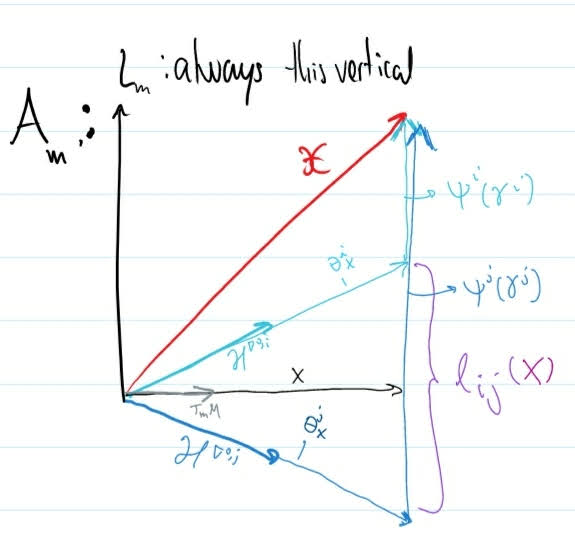
\includegraphics[width = \textwidth/2]{images/DiagramaMapasLocalesAlgebroide.jpg}
%     \caption{Representation of the local maps introduced to study a transitive Lie algebroid $A$. The whole space represents, roughly, the vector space $A_m$ for $m \in M$, and $\oid X$ such that $a(\oid X) = X$ is an arbitrary element in $A_m$. Understanding $j$ as an inclusion, the vertical axis represents the adjoint Lie algebroid fiber $L_m$. The horizontal axis represents the tangent space $T_m M$, but it is not part of $A_m$, since there is no canonical horizontal direction in $A_m$. The images of $\nabla^{0,i}$ and $\nabla^{0,j}$ give two distinct notions of horizontality in $A_m$.}
%     \label{fig:localMaps}
% \end{figure}

\todo{Reconstruction THeorem?}

\lin

When making practical calculations with transitive Lie algebroids, the algebraic perspective of Lie algebroids is usually simpler to work with and more useful. Based on the fact that that the space of section $\Gamma(TU\times \alg g)$ of a transitive Lie algebroid over a manifold $U$ is canonically isomorphic to $\Gamma(TU) \oplus C^\infty(U, \alg g)$, the following are the algebraic versions of the vector bundle maps defined in this section:
\begin{align*}
    &\psi_i:& C^\infty(U_i, \alg g) &\to \Gamma_{U_i}(L)\\
    &\nabla^{0, i}:& \Gamma(TU_i) &\to \Gamma_{U_i}(A)\\
    &S_i:& \Gamma(TU_i)\oplus C^\infty(U_i, \alg g) &\to \Gamma_{U_i}(A)\\
    &\alpha^i_j:& C^\infty(U_{ij}, \alg g) &\to C^\infty(U_{ij}, \alg g) \\
    \text{or   } &\alpha^i_j& \in C^\infty(U_{ij}, \alg{gl}(\alg g)) \\
    &l^i_j:& \Gamma(TU_i) &\to \Gamma_{U_i}(L)\\
    &\chi^i_j:& \Gamma(TU_i) &\to C^\infty(U_{ij}, \alg g) \\
    &S^i_j:& \Gamma(TU_i)\oplus C^\infty(U_{ij}, \alg g) &\to \Gamma(TU_i)\oplus C^\infty(U_{ij}, \alg g).
\end{align*}

\subsection{Local version of some concepts} \label{chBasicsubsectionLocalVersion}
\improvement{Agregue este titulo}
Let us now see the local version of some important concepts.

% \begin{remark}
% \label{remarkFamilyLocalTrivializationsMorphismOfTransitiveLieAlgebroid}
Let $\psi: A \to A'$ be a morphism between transitive Lie algebroids. Once trivializing neighborhoods $\{U_i\}_{i \in I}$ for both $A$ and $A'$ have been chosen, $\psi$ can be encoded as a family $\{(\omega_i, \psi_{+, i})\}_{i\in I}$ of representations $\psi_i = a \oplus (\omega_i + \psi_{+,i})$ between trivial Lie algebroids as suggested by example \ref{exampleAllRepresentationsofTLAoverTrivialVectorbundle}.
% \end{remark}

\lin

% \begin{remark}
% \label{remarkFamilyLocalTrivializationsRepresentationsOfTransitiveLieAlgebroid}
Similarly, let $\phi: A \to \alg D(E)$ be a representation for the transitive Lie algebroid $A$, and suppose that $\{U_i\}_{i\in I}$ is an open cover trivializing both $A$ and $E$. Based on example \ref{exampleAllRepresentationsofTLAoverTrivialVectorbundle}, the representation $\phi$ can be encoded as a family $\{(B_i, \phi_{L, i})\}_{i\in I}$ of representations $\phi_i = a \oplus (B_i + \phi_{L,i})$ of trivial Lie algebroids $TU_i \times \alg g$ on trivial vector bundles $U_i \times V$, where $\alg g$ is the typical fiber of the vertical part of $A$, and $V$ is the typical fiber of $E$. The following examples show that the representations of the trivializing Lie algebroids of an algebroid that locally trivialize the trivial and adjoint representations, respectively, are already known representations.
% \end{remark}

\begin{example}\label{exampleTrivializationOfTrivialRepresentationIsTrivialRepresentation}
Let $A$ be acting on the trivial vector bundle $E = M \times V$ by the trivial representation $\phi = a$. On a trivializing neighborhood $U_i$ of $A$ the trivialization of $\phi$ is once again a trivial representation:
\begin{align*}
    \phi_i(X \oplus \eta) &= \phi(S(X \oplus \eta))\\
        &= a(S(X \oplus \eta))\\
        &= a(X \oplus \eta);
\end{align*}
to pass to the second line we used the fact that $S$ respects the anchor. This, in particular, means that every $B_i$ and $\phi_{L, i}$ are $0$.
\end{example}

\begin{example}\label{exampleTrivializationOfAdjointRepresentationIsAdjoint}
Let $A$ act on $L$ through the adjoint representation $\phi = ad$. Then the local trivialization of $\phi$ over a neighborhood that trivializes $A$ is again an adjoint representation. Assume without lose of generality that the injection $j$ is an inclusion:
\begin{align*}
    \phi_i(X \oplus \eta)\theta &= \psi_i^{-1} \comp \phi(S_i(X \oplus \eta)) \comp \psi_i(\theta)\\
       &= \psi_i^{-1} ( [S_i(X \oplus \eta), \psi_i(\theta)] )\\
       &= \psi_i^{-1} ( [\nabla^{0,i}_X \oplus \psi_i(\eta), \psi_i(\theta)] )\\
       &= \psi_i^{-1}[\nabla^{0, i}_X, \psi(\theta)] + \psi^{-1}[\psi_i(\eta), \psi_i(\theta)]\\
       &= X(\theta) + [\eta, \theta]\\
       &= [X \oplus \eta, \theta]\\
       &= ad(X \oplus \eta, \theta).
\end{align*}
\end{example}

An important family of representations are associated to the representation of a Lie group as seen in example \ref{equationGroupInducedRepresentationInTrivialAlgebroids}. Let $G$ be a group with Lie algebra $\alg g$, and the vector space $V$ be a representation space of $G$. Suppose that $A$ is a transitive Lie algebroid with $\alg g$ as the typical fiber of its vertical part, and let $V$ be a vector space on which $G$ acts. Let $U_i$ and $U_j$, $U_{ij} \neq \emptyset$ be open subsets of $M$ that trivialize $A$. If we allow $TU_i \times \alg g$ and $TU_j \times \alg g$ to be represented in $U_i \times V$ and $U_j \times V$, respectively, via the group representation \eqref{equationGroupInducedRepresentationInTrivialAlgebroids}, we can ask ourselves \rtext{¿what conditions need to be satisfied for those representations to be the trivializations of a global representation of $A$ on a vector bundle $E$ that trivializes over $U_i$ and $U_j$?} Letting $\beta^i_j = \beta_i^{-1} \comp \beta_j : U_{ij} \times V \to U_{ij} \times V$ be the transition function of $E$ from $U_j$ to $U_i$, a quick analysis shows some conditions are imposed on them: let $\mu$ be a section on $E$ such that $f \in C^\infty(U_{j}, V)$ is its trivialization over $U_i$, i.e. $\beta_i(f) $ be the trivialization of a section $\mu \in \Gamma(E)$, hence $\beta_j(f) = \mu|_{U_j}$, then the compatibility condition 
\begin{equation}
    \beta_j^i[(X \oplus \eta) f] = X \oplus (\chi^i_j(X) + \alpha^i_j(\eta))\beta^i_j(f)
\end{equation}
must be satisfied for any $X \oplus \eta \in \Gamma(TU_i) \oplus C^\infty(U_{ij}, \alg g)$, where $\chi^i_j$ and $\alpha^i_j$ are the pasting maps \eqref{equationDefinitionOfChiGeneral} and \eqref{equationDefinitionOfAlphaGeneral} for $A$ over $U_{ij}$. The previous equation decomposes in the following equations restricting the values of $\beta^i_j$:
\begin{align}
    \chi^i_j(X) \cdot \beta^i_j(f) &= X(\beta^i_j)f\\
    \alpha^i_j(\eta)(\beta^i_j(f)) &= \beta^i_j(\eta \cdot f).
\end{align}
The fact that $\chi^i_j$ is a Maurer-Cartan form, that $\alpha^i_j$ is a LAB morphism, and the compatibility conditions between $\chi^i_j$ and $\alpha^i_j$ should impose further restrictions on what the transition function $\beta^i_j$ can be, perhaps even characterizing them; however, on the literature that was reviewed no further analysis was found. We will see in example \ref{exampleLocalTrivializationOfGroupInducedRepresentationOfAtiyahLieAlgebroidAction} that in the case of the standard representation of a principal bundle on an associated vector bundle these conditions are satisfied.


%%%%%%%%%%%%%%%%%%%%%%%%%%%%%%%%%%%%%%%%%%%%%%%%%%%%%%%%%%%%%%%%%%%%%%%%%%%%%%%%%%%%
%%%%%%%%%%%%%%%%%%%%%%%%%%%%%%%%%%%%%%%%%%%%%%%%%%%%%%%%%%%%%%%%%%%%%%%%%%%%%%%%%%%%
\subsection{Local Description of the Atiyah Lie algebroid}

Let $G \to P \to M$ be a (smooth) principal bundle, and let $\alg g$ be the Lie algebra of the Lie group $G$. Since this is the family of examples that appear in traditional gauge theories, some time will be devoted to its understanding.

Throughout this section $\{(U_i, \rho_i: U_i \times G \to P|_{U_i})\}_{i \in I}$ will denote a principal bundle atlas, $\mathcal U_i = P|_{U_i} = \pi^{-1}(U_i)$ and $\sigma_i: U_i \to \mathcal U_i$ will denote the corresponding trivializing local sections, which satisfy
\begin{eqnsplit*}
    \rho_i: U_i \times G &\to \mathcal U_i\\
            (m, g) &\mapsto \sigma_i(m) g.
\end{eqnsplit*} Finally, let $g_{ij}: U_{ij} = U_i \inter U_j \to G$ be the transition functions of the atlas satisfying, for any $m \in U_{ij}$,
\begin{eqnsplit}
    \label{transitionFunctionDefn}
    \sigma_i(m) &= \sigma_j(m) g_{ji}(m)\\
    \rho_i(m, g) &= \rho_j(m, g_{ji}(m) g).
\end{eqnsplit}
From this principal bundle atlas, we will now build a Lie algebroid atlas for the Atiyah Lie algebroid $TP/G$. Since we are identifying the spaces of sections of the Atiyah sequence with some other $C^\infty(M)$-modules, we will also understand the relevant maps in terms of this spaces.

We will now build a Lie algebroid atlas on $TP/G$ based on a trivialization of the principal bundle $P$. For the rest of this section suppose that the open cover $\{U_i\}_{i \in I}$ of $M$ is associated to a manifold trivialization of $M$ and to a principal bundle trivialization of $P$ with local sections $\sigma_i: U_i \to P|_{U_i}$.

\noindent Recall the map $j$ of the Atiyah sequence \ref{definitionAtiyahSequencePrincipalBundleVectorBundle}. For any $p \in P$ and $\eta \in \alg g$, the immersion and injective Lie algebroid morphism $j$ is defined by equation (\ref{formulaJ}):
\begin{eqnsplit*}
    j: P \times \alg g/G &\to T^\pi P/G \subset TP/G\\
    \cl{p, \alg \eta} &\mapsto \cl{\der{t}[t = 0] p \exp{(-t \alg \eta)}}.
\end{eqnsplit*}
It induces the $C^\infty(M)$-module and Lie algebra morphism of equation (\ref{formulaJbar}):
\begin{eqnsplit*}
    \up{j} : C^\infty_G(P, \alg g) &\to \Gamma^G(TP)\\
    \up{j}(\stilde \eta)(p) &= \der{t}[t = 0] p \exp(-t \stilde \eta(p))
\end{eqnsplit*}


\begin{definition}\label{definitionPsiAtiyah}
For each $i \in I$, define the LAB morphism, i.e. vector bundle morphism that respects the fiberwise Lie brackets,
\begin{eqnsplit}
    \psi_i: U_i \times \alg g  \to &\mathcal U_i \times \alg g/G \\
    (m, \eta) \mapsto &\cl{\sigma_i(m), \eta} \\
                   &= \cl{\sigma_i(m)g, Ad_{g^{-1}} \eta}  \quad \textrm{for any $g \in G$}.
\end{eqnsplit}
It induces $C^\infty(M)$-module and Lie algebra morphism
\begin{eqnsplit}
    \tilde \psi_i: C^\infty(U_i, \alg g) &\to C^\infty_G(\mathcal U_i, \alg g) \\
    \stilde \eta &\mapsto (\sigma_i(m)g \mapsto Ad_{g^{-1}}(\stilde \eta(m)))  \quad \textrm{for any $m \in M$, $g \in G$}.
\end{eqnsplit}
\end{definition}


\begin{definition}\label{definitionNabla0iAtiyah}
For each $i \in I$, define the Lie algebroid morphism
\begin{eqnsplit}
    \nabla^{0,i}: TU_i \to & T\mathcal U_i/G \\
             X \mapsto &\cl{\sigma_{i*}(X)}.
\end{eqnsplit}
It induces $C^\infty(M)$-module and Lie algebra morphism
\begin{eqnsplit}
    \up \nabla^{0,i}: \Gamma(TU_i) &\to \Gamma^G(T\mathcal U_i) \\
    \sect X &\mapsto (\sigma_i(m)g \mapsto R_{g*}\sigma_{i*}(X)),
\end{eqnsplit}
for all $m \in M$, $g \in G$.
\end{definition}

\begin{theorem}\label{algebroidAtlasAtiyah}
An open cover of $M$ that corresponds to trivializes both the principal bundle $G \to P \to M$ and the manifold atlas of $M$ produce a Lie algebroid atlas on $0 \to P \times \alg g/G \xrightarrow{j} TP/G \xrightarrow{a} TM \to 0$ through the maps $\psi_i:U_i\times \alg g \to P\times \alg g/G|_{U_i}$ defined in \ref{definitionPsiAtiyah}, and the maps $\nabla^{0,i}: TU_i \to TP/G|_{U_i}$ defined in \ref{definitionNabla0iAtiyah}.
\end{theorem}
\begin{proof}
For any $m \in M$ and $\eta,\theta \in \alg g$
\begin{equation*}
    \psi_i(m, [\eta, \theta]) = \cl{\sigma_i(m), [\eta, \theta]} = [\cl{\sigma_i(m), \eta}, \cl{\sigma_i(m), \theta}],
\end{equation*} hence $\psi$ is indeed a LAB morphism.

Since $\sigma_i$ is a local section of the projection $\pi: P \to M$, $\pi_*(\sigma_{i*}(X)) = X$, hence $\nabla^{0,i}$ respects the anchor. is Lie algebroid morphism. That's what it induces

Given the definitions we have studied throught this chapter of the Atiyah Lie algebroid and its bracket, the compatibility condition of the suggested atlas reduces to verifying that $[\up{\nabla^{0,i}}(\sect X), \up{j \psi(\sect \eta)}] = \up j(\tilde \psi_i(\sect X(\stilde \eta))) \in C^\infty_G(P)$ for all $\sect X \oplus \sect \eta \in \Gamma(TU_i) \oplus C^\infty(U_i, \alg g)$. This is done using the flow of $\up{\nabla^{0,i}}(\sect X)$ and the definition of the Lie derivative of vector fields on $P$.\improvement{Agregue esto}
\end{proof}

The components of a Lie algebroid atlas combine to give the trivialization morphism:
\begin{definition}\label{definitionTrivializationSAtiyahAlgebroid}
For any $i \in I$, define the Lie algebroid morphism
\begin{eqnsplit}
    S_i: TU_i \oplus (U_i \times \alg g) \to& T\mathcal U_i/G \\
    X \oplus \eta &\mapsto \nabla^{0,i}(X) + j \psi_i(\eta)\\
    &= \cl{\sigma_{i*}(X) + \der{t}[t = 0]\sigma_i(m) \exp{(-t \eta)}}.
\end{eqnsplit}
This map induces the $C^\infty(M)$-linear and Lie algebra morphism:
\begin{eqnsplit*}
    \up{S_i}: \Gamma(TU_i)\oplus C^\infty(U_i, \alg g) \to  \Gamma^G(T \mathcal U_i)
    \end{eqnsplit*}
given by 
\begin{eqnsplit}
    \sect X \oplus \stilde \eta &\mapsto \left(\sigma_i(m) g \mapsto R_{g*}\sigma_{i*}(X) + \der{t}[t=0] \sigma_i(m)\exp{(-t \stilde \eta(m))} g\right)
\end{eqnsplit} for any $m \in U_i$ and $g \in G$.
This is called the \emph{trivializing Lie algebroid morphism of $TP/G$ over $U_i$}.
\end{definition}

\lin

We now study the pasting maps between trivializations of the Atiyah Lie algebroid associated to the Lie algebroid atlas previously defined.

\begin{proposition}\label{propositionAlphaijAtiyahTransitionAdjointIs}
For any $i, j \in I$ such that $U_i \inter U_j \neq \emptyset$, the transition maps of the adjoint Lie algebroid associated to the LAB atlas $\{\psi_i: U_i \times \alg g \to \mathcal U_i \times \alg g/G\}$ are
\begin{eqnsplit}
    \alpha^i_j: U_{ij} \times \alg g &\to U_{ij} \times \alg g\\
    (m, \eta) &\mapsto (m, Ad_{g_{ij}(m)} \eta).
\end{eqnsplit} On sections it can induces the map,
\begin{eqnsplit}
    \alpha^i_j:C^\infty(U_{ij}, \alg g) & \to C^\infty(U_{ij}, \alg g)\\
    \stilde \eta &\mapsto Ad_{g_{ij}} (\stilde \eta)
\end{eqnsplit} 
for all $\stilde \eta \in C^\infty(U_{ij}, \alg g)$.
If $G$ is matrix Lie group, this can also be written as:
\begin{align}
    \alpha^i_j(\stilde \eta) = g_{ij} \stilde \eta {g_{ij}}^{-1}.
\end{align} 

\end{proposition}\label{propositionlijAtiyahIs}
\begin{proof}
For any $m \in U_{ij}$ and $\eta \in \alg g$,
\begin{align*}
    \alpha^i_j(m, \eta) &= \psi_i^{-1}(\cl{\sigma_j(m), \eta})\\
      &= \psi_i^{-1}(\cl{\sigma_i(m)g_{ij}(m), \eta})\\
      &= \psi_i^{-1}(\cl{\sigma_i(m), Ad_{g_{ij}(m)} \eta})\\
      &= (m, Ad_{g_{ij}(m)} \eta),
\end{align*}
as desired.
\end{proof}

\begin{proposition}\label{propositionChiijTransitionFormsAre}
For any $i, j \in I$ such that $U_{ij} \neq \emptyset$, define the $\mathcal U_{ij} \times \alg g/G$-valued forms on $U_{ij}$
\begin{eqnsplit}
    l^i_j: TU_{ij} \to& \mathcal U_{ij} \times \alg g/G \\
        X &\mapsto j^{-1}(\nabla^{0,j}(X) - \nabla^{0,i}(X))\\
        &= \cl{\sigma_i(m), L_{g_{ij}(m)*}(g^{-1}_{ij*} (X))}
\end{eqnsplit} for $m = \pi(X)$. If $G$ is a matrix Lie group, it is then true that:
\begin{align}
    l^i_j(X) = \cl{\sigma_i(m), g_{ij}(m) dg^{-1}_{ij}(X)},
\end{align}
where $dg^{-1}_{ij}$ denotes the $1$-form-valued matrix that results from applying on each entry the differential $d$ of differential forms on $U_{ij}$.
\end{proposition}
\begin{proof}
Let $X \in T_m U_{ij}$ be tangent to the path $\gamma$ on $U_{ij}$ such that $\gamma'(0) = m \in TU_{ij}$. Then
\begin{align*}
    \sigma_{i*}(X) &= \der{t}[t=0]{\sigma_i(\gamma(t))}\\
       &= \der{t}[t=0]{\sigma_j(\gamma(t))g_{ij}^{-1}(\gamma(t))}\\
       &= \der{t}[t=0]{\sigma_j(m)\gamma_{ij}^{-1}(\gamma(t))} 
       + \der{t}[t=0]{\sigma_j(\gamma(t))g^{-1}_{ij}(m)}\\
       &= \der{t}[t=0]{\sigma_i(m)\gamma_{ij}(m)\gamma_{ij}^{-1}(\gamma(t))}
       + \der{t}[t=0]{\sigma_j(\gamma(t))g^{-1}_{ij}(m)} \\
       &= \left[ L_{g_{ij}(m)*}(g_{ij*}^{-1}(X)) \right]^*_{\sigma_i(m)} + \der{t}[t=0]{\sigma_j(\gamma(t))g^{-1}_{ij}(m)};
\end{align*}
recall that the notation $[\eta]^*_p$ denotes the left invariant vector field on $TP$ generated by $\eta \in \alg g$ at $p \in P$. Now,
\begin{align*}
    \nabla^{0,j}_X - \nabla^{0,i}_X &= \cl{\sigma_{j*}(X)} - \cl{\sigma_{i*}(X)} \\
    &= \cl{\sigma_{j*}(X) g_{ij}^{-1}(X) - \sigma_{i*}(X)}\\
    &= \cl{- [L_{g_{ij}(m)*}(g_{ij*}^{-1}(X))]^*_{\sigma_i(m)}}.
\end{align*}
Hence
\begin{align*}
    l^i_j(X) &= j^{-1}(\nabla^{0,j}_X - \nabla^{0,i}_X)\\
      &= \cl{\sigma_i(m), L_{g_{ij}(m)*}(g_{ij*}^{-1}(X))}.
\end{align*}
Recall that $L_{g_{ij}(m)*}(g_{ij*}^{-1}(X)) = \der{t}[t=0]{g_{ij}(m) g^{-1}_{ij}(\gamma(t))}$. If $G$ is a matrix Lie group, we can take $g_{ij}(m)$ outside the derivative and apply the derivative entry-wise, hence the last result follows.
\end{proof}

Having a formula for the maps $l^i_j$ the pasting $1$-forms of the local trivialization are now clear:
\begin{proposition}\label{propositionChisForAtiyah}
For any $i, j \in I$ such that $U_i \inter U_j \neq \emptyset$, the transition $\alg g$-valued Maurer-Cartan forms over $U_{ij}$ associated to the given Lie algebroid atlas of the Atiyah lie algebroid sequence $0 \to P \times \alg g/ G \to TP/G \to TM \to 0$ are
\begin{eqnsplit}
    \chi^i_j: TU_{ij} \to& U_{ij} \times \alg g \\
        X &\mapsto \psi_i^{-1} \circ l^i_j(X)\\
        &= \left(\sigma_i(m), L_{g_{ij}(m)*}(g^{-1}_{ij*} (X))\right)
\end{eqnsplit} where $m = \pi(X)$ and $L$ is the left multiplication map in $G$. If $G$ is a matrix Lie group, on a vector field $\sect{X} \in \Gamma(TU_{ij})$ this becomes:
\begin{align}
    \chi^i_j(X) = \left(m, g_{ij}(m) dg^{-1}_{ij}(X)\right).
\end{align}
\end{proposition}

If $\{\sect X \oplus \stilde \eta^i\}$ is a family of local trivializations of $\oid X \in \Gamma(TP/G)$, and supposing that $G$ is a matrix Lie group, we may combine the previous propositions to find the following relation between local trivializations over open sets $U_{ij} \neq \emptyset$:
\begin{align}\label{equationCHangeOfCoordinatesAtiyahSectionsMatrixGroup}
    \sect{X} \oplus \stilde \eta^i &= \sect{X} \oplus (g_{ij} \stilde \eta^j g_{ij}^{-1} + g_{ij} dg^{-1}_{ij}(\sect X))
\end{align}

%TODO: general form of a section of $TP/G$ as section of $TP$

\begin{example}[Local trivialization of representation of $TP/G$ on $E = P \times V/G$]\label{localTrivializationOfRepresentationOfAtiyahTPGonAssociated}
\label{exampleLocalTrivializationOfGroupInducedRepresentationOfAtiyahLieAlgebroidAction}
Suppose that the open $U_i$ trivializes $E$ as $\beta_i: U_i \times V\to E|_{U_i}$. Let $\eta \in C^\infty(U_i, \alg g)$, $f \in C^\infty(U_i, V)$ be arbitrary. Then
$$(\upsect{S_i(X \oplus \eta)})_{\sigma_i(m)} = \sigma_{i, *}(X) + \der{t}[t=0]{\sigma_i(m) \cdot \exp[-t \eta(m)]} \in T_{\sigma_i(m)} P$$
and
$$\upsect{\beta_i(f)}: \sigma_i(m)g \mapsto g^{-1} f(m)) \in C^\infty_G(P, V)$$.
Therefore:
\begin{align*}
    \beta_i^{-1}[\phi\comp S_i(X \oplus \eta)&(\beta_i(f))] (m)
        = \upsect{\phi \comp S_i(X \oplus \eta)}_{\sigma_i(m)} (\upsect{\beta_i(f)})\\
        %&= \sout{\upsect{\phi\cl{\sigma_{i, *}(X)}}_{\sigma_i(m)} (\upsect{\beta_i(f)}) + \upsect{\phi( j\psi_i(\eta))}_{\sigma_i(m)} (\upsect{\beta_i(f)})}\\
        &= \sigma_{i, *}(X_m)(\upsect{\beta_i(f)}) 
        + \der{t}[t = 0]{\upsect{\beta_i(f)}(\sigma_i(m) \cdot \exp[-t \eta(m)])}\\
        &= \der{t}[t = 0]{\sigma_i(\gamma(t))} (\upsect{\beta_i(f)}) + \der{t}[t=0]{\exp[t \eta(m)] f(m)}\\
        &= \der{t}[t=0]{f(\gamma(t))} + (\eta \cdot f)(m)\\
        &= X_m(f) + (\eta \cdot f)(m),
\end{align*}
where $\gamma: I \to U_i$ is a path on $M$ such that $\gamma'(0) = X_m$. We conclude that the local trivialization $\phi_i: TU_i \times \alg g \to \alg D(U_i \times V)$ of the representation $\phi: TP/G \to P \times V/G$ is
\begin{equation}\label{equationLocalRepresentationAtiyahLieAlgebroidOnAssociatedVectorBundleExpectedTrivialALgebroidRepresentationActionOfGroup}
    \phi_i(X \oplus \eta)(f) = X(f) + \eta \cdot f,
\end{equation}
i.e. it is the group induced representation (example \ref{equationGroupInducedRepresentationInTrivialAlgebroids}).
\end{example}




\subsection{Examples}
%%%%%%%%%%%%%%%%%%%%%%%%%%%%%%%%%%%%%%%%%%%%%%%%%%%%%%%%%%%%%%%%%%%%%%%%%%%%%%%%%%%%
%%%%%%%%%%%%%%%%%%%%%%%%%%%%%%%%%%%%%%%%%%%%%%%%%%%%%%%%%%%%%%%%%%%%%%%%%%%%%%%%%%%%

 We have seen \ref{definitionAtiyahSequencePrincipalBundleVectorBundle} that to every principal bundle $G \to P \to M$ there is an associated a transitive Lie algebroid with Atiyah sequence $0 \to P \times \alg g / G \to TP/G \to TM \to 0$. Furthermore, theorem \ref{algebroidAtlasAtiyah} states that local trivializations of $P$ and $M$ induce local trivializations of the Lie algebroids $P \times \alg g/G$ and $TP/G$. We will now give a description of some principal bundles over projective spaces isomorphic to spheres which will have a trivializations with only $2$ charts for both the manifold and the principal bundle, each of which covers all but one point. This easily shows us that a version of the reconstruction theorem applies, at least for these Lie algebroids over spheres, where \rtext{the necessary maps to reconstruct the Lie algebroid are the transition maps $\alpha^i_j$ of \ref{propositionAlphaijAtiyahTransitionAdjointIs} and $\chi^i_j$ of \ref{propositionChiijTransitionFormsAre}}.
 The $\alpha$ maps are the transition functions of the adjoint Lie algebroid $P \times \alg g/G$, so our first task will be to understand the Lie algebras $\alg g$ to then understand the trivializations and the transition functions.
%     \begin{itemize}
    
%     \item Complex Hopf bundle, as $S^1 \rightarrow S^3 \to S^2$ and as $S^1 \rightarrow S^3 \to \CC P^1$
    
%     \item One generalization: the principal bundles $S^1 \rightarrow S^{2n - 1} \to \CC P^{n-1}$
    
%     \item Another generalization: the principal bundles $S^1 \rightarrow P^k \to S^2$
    
%     \item Quaternionic Hopf bundle, as $S^3 \hookrightarrow S^7 \to S^4$ and as $S^3 \hookrightarrow S^7 \to \HH P^1$
    
%     \item One generalization (which I'll probably ignore): the principal bundles $S^3 \hookrightarrow S^{4n - 1} \to \HH P^{n-1}$
    
%     \item Another generalization: the principal bundles $S^3 \hookrightarrow P^k \to S^4$
    
%     \end{itemize} 
The examples that will be developed throughout this document are those associated to the principal bundles $S^1 \to P^k \to S^2$ and $S^3 \to P^k \to S^4$ One of our examples, the Atiyah Lie algebroid associated to the complex Hopf bundle, has a simple structure that allows it to be pictured without using local trivializations, so we will develop in this ``global'' language mainly to acquire intuition on the manipulations that are made in this context. % by studying the local trivializations induced by the principal bundle trivialization. In the case of the complex Hopf bundle we can give a partial global description thanks to the local frames $\set{\partial_\phi, \partial_\theta}$ of $TS^2$ and $\set{\partial_\phi, \partial_{\xi^1}, \partial_{\xi^2}}$ of $TS^3$.

\subsubsection{Lie algebras and transition functions of adjoint algebroid}
%%%%%%%%%%%%%%%%%%%%%%%%%%%%%%%%%%%%%%%%%%%%%%%%%%%%%%%%%%%%%%%%%%%%%%%%%%%%%%%%%%%%


The Lie algebra of the Lie group $S^1$ is $i\RR \subset \CC$, which can be easily seen since every element of $g \in S^1$ may be written as $g = e^{i r}$ for some $r \in \RR$. A basis of this algebra is simply $\set{i} \subset i\RR$, with only one element and so the Lie bracket is trivially $0$. $S^1$ can be canonically identified with $U(1)$, so its Lie algebra can be seen \dbtext{embedded} in the associative matrix Lie algebra $iM_1(\RR) \subset M_1(\CC)$, so the adjoint action of any $g \in U(1)$, $Ad_g: iM_1(\RR) \to iM_1(\RR)$, is given by the matrix multiplication $(ir) \mapsto g(ir)g^{-1}$, but $M_1(\CC)$ is a commutative algebra, implying that \[Ad_g = Id : i\RR \to i\RR\] for any $g \in S^1$.

Hence, the first pasting map, the transition functions $\alpha^N_S$ of \ref{propositionAlphaijAtiyahTransitionAdjointIs} for the Atiyah Lie algebroids $0 \to P^k \times i\RR/S^2 \to TP^k/S^1 \to TS^2 \to 0$, $k \in \ZZ_{\geq 0}$, are
\begin{eqnsplit}
    \alpha^N_S = Id = \alpha^S_N,
\end{eqnsplit}
where this identity may refer to both the identity as LAB maps $\alpha^i_j:U_{SN} \times i\RR \to U_{SN}\times i\RR$, as well as elements of $C^\infty(U_{SN}, \alg{gl}(i\RR))$.

\lin

To understand the Lie algebra associated to our second family of principal bundles, we first study the space $Im \HH := \{x i + y j + z k \st (x, y, z) \in \RR^3 \} \subset \HH$, whose elements we denote, by abuse of notation, $\vec x := x i + y j + z k \in Im \HH \cong \RR^3$. The product of two elements $\vec x, \vec y$ of this subspace of the associative normed algebra $\HH$ is 
\begin{align*}
    \vec x \vec y &= \frac{1}{2}(\vec x \vec y - \vec y \vec x) - \frac{1}{2}(\vec x \vec y + \vec y \vec x) \\
    &= \vec x \times \vec y - \vec x \cdot \vec y \in \HH
\end{align*} where the $\times$ and $\cdot$ operations are the cross product and dot product of the corresponding vectors in $\RR^3$. The induced commutator is, then,
\begin{align}
    [\vec x, \vec y] = 2 (\vec x \times \vec y) \in Im \HH,
\end{align} showing that $Im \HH$ is a real Lie algebra, which has as basis the set $\{i, j, k\}$ that satisfy the commutation relations
\begin{align}
    [i, j] = 2k && [j, k] = 2i && [k, i] = 2i. 
\end{align} 

We now wish to see what is the (unique) simply connected Lie group $G \subset \HH$ associated to the Lie algebra $Im \HH$. Given an arbitrary $\vec x \in Im \HH$, the exponential $e^{x^1 i + x^2 j + x^3 k}$ is unitary, so the Lie group $G$ we search is a subgroup of $S(\HH)$. Now, recall that the real Lie algebra $\alg{su}(2)$ of $SU(2)$ of anti-hermitian matrices is generated by the basis $\set{u_1, u_2, u_3} \subset \alg{su(2)}$ where $u_i = i \sigma_i$, $i = 1, 2, 3$ and
\begin{align}
    \sigma_1 = \begin{pmatrix} 0 & 1 \\ 1 & 0 \end{pmatrix} && \sigma_2 = \begin{pmatrix} 0 & -i \\ i & 0 \end{pmatrix} && \sigma_1 = \begin{pmatrix} 1 & 0 \\ 0 & -1 \end{pmatrix},
\end{align} where this basis satisfy the bracket in $\alg{su}(2)$ is determined by the relations
\begin{align}
    [u_1, u_2] = 2u_3 && [u_2, u_3] = 2u_1 && [u_3, u_1] = 2u_2. 
\end{align} 
hence the following is an isomorphism of real Lie algebras
% \begin{equation}
% \begin{tikzcd}
%     Im \HH \arrow{r}{\cong} & \alg{su}(2) \\
%     i \arrow[mapsto]{r} & i\sigma_1 \\
%     j \arrow[mapsto]{r} & i\sigma_2 \\
%     k \arrow[mapsto]{r} & i\sigma_3 \\
%     \vec x \arrow[mapsto]{r} & \vec x \cdot \vec \sigma = \begin{pmatrix} x^3 & x^1 -i x^2  \\ x^1 + ix^2  & -x^3\end{pmatrix}
% \end{tikzcd}
% \end{equation} 
\begin{eqnsplit}
    Im \HH \overset{\cong}{\longrightarrow}& \alg{su}(2) \\
    i \longmapsto & i\sigma_1 \\
    j \longmapsto & i\sigma_2 \\
    k \longmapsto & i\sigma_3 \\
    \vec x \longmapsto & i\vec x \cdot \vec \sigma = \begin{pmatrix} ix^3 & x^2 + ix^1  \\ -x^2 + ix^1  & -ix^3\end{pmatrix}.
\end{eqnsplit}
This algebra isomorphism induces the isomorphism of smooth Lie groups
\begin{eqnsplit}
    G \subset S(\HH) \overset{\cong}{\longrightarrow} & SU(2) \cong S^3 \\
    e^{x^1 i + x^2 j + x^3 k} \longmapsto & e^{i(x^1 \sigma_1 + x^2 \sigma_2 + x^3 \sigma_3)},
\end{eqnsplit}
but then the simply-connected Lie group $G$ associated to the Lie algebra $Im \HH$ is precisely $S(\HH) \equiv S^3$. All of this allows us to conclude that we can naturally use $Im \HH$ as the Lie algebra for $S^3$.


% Every element $q \in \HH$ can be written as
% \begin{align*}
%     q &= e^{x^ 0 + x^1 i + x^2 j + x^3 k} & \text{for some } x^0 \in \RR, \vec x = (x^1, x^2, x^3) \in \RR^3 \\
%      &= e^{x^0} e^{x^1 i + x^2 j + x^3 k}\\
%      &= e^{x^0} \left( \cos |\vec x|  + \hat x \sin|\vec x| \right) \in \HH
% \end{align*}
% where $\hat x \in \HH$, by abuse of notation, denotes the quaternion $\hat x = \frac{x^1 i + x^2 j + x^3 k}{\sqrt{(x^0)^2} + (x^1)^2 + (x^3)^2}$ associated to the unitary $\RR$ vector $\hat x = \frac{\vec x}{||\vec x||}$, its conjugate is
% \begin{align*}
%     \conj{q} = e^{x^ 0 - x^1 i - x^2 j - x^3 k},
% \end{align*}
% its norm is
% \begin{align*}
%     |q| &= \sqrt{q \conj{q}} \\
%      &=e^{x^0}
% \end{align*}
% and its inverse is
% \begin{align*}
%     q^{-1} = \conj{q}/|q|^2.
% \end{align*} 
% From all of this it is easy to see that \otext{the unitary quaternions, which coincide as a set with $S^3 \subset \HH \equiv \RR^4$, are a smooth Lie group whose real Lie algebra is $Im \HH$}.


Finally, for every $e^{\vec x} = \cos |\vec x| + \hat x \sin |\vec x|  \in S^3$ the adjoint action 
\begin{eqnsplit}
    Ad_{e^{\vec x}}: Im \HH &\to Im \HH\\
     \vec y &\mapsto e^{\vec x} \, \vec y \, e^{-\vec x} = R_{\hat x, |\vec x|}(\vec y)
\end{eqnsplit}
is the rotation operation of $|\vec x|$ radians in $\RR^3$ with respect to the axis $\hat x$.




%\begin{remark}\label{remarkAlphaAndChiSufficeSn}{For the principal bundles we have been working with, the open cover $\set{U_S, U_N}$ trivializes both the base space $S^n$ and the principal bundles, so \rtext{we get a full description of the transitive Lie algebroids by describing exactly two maps: $\alpha^N_S$ and $\chi^N_S$}}.
%\end{remark}

\subsubsection{Transition algebra-valued forms}
%%%%%%%%%%%%%%%%%%%%%%%%%%%%%%%%%%%%%%%%%%%%%%%%%%%%%%%%%%%%%%%%%%%%%%%%%%%%%%%%%%%%

To complete the description of the Atiyah Lie algebroid associated to the principal bundles $P^k$ from transition functions given the open cover $\{U_S, U_N\}$ we only need the Lie algebra-valued Maurer-Cartan forms $\chi^N_S = - \chi^S_N$ found in proposition \ref{propositionChiijTransitionFormsAre} to be $\chi^N_S = g_{NS} dg_{NS}^{-1} = - \chi^S_N$ since the structure groups $S^3$ and $S^1$ are isomorphic to the matrix Lie groups $SU(2)$ and $U(1)$, respectively.

For the Lie algebroids over $S^2$, with transition function $g_{NS} = e^{ik\theta} \in C^\infty(U_{SN}, S^1)$ it then follows that the form $\chi^N_S: \Gamma_{U_{SN}} \to C^\infty(U_{SN}, i\RR)$
\begin{eqnsplit}
     \chi^N_S &= -ikd\theta\\
     \chi^S_N &= +ik d\theta.
\end{eqnsplit}


% \[j\cl{[p, e^{i \alpha}, N], ir} \mapsto \cl{\frac{d}{dt}|_{t=0} [p, e^{i\alpha}e^{-irt}, N]}\]

% $x: V \subset \RR^2 \to U_{CS} \subset S^2$ can be any coordinate map that exists in a neighborhood of the point $x(x^1, x^2) \in U_{SN}$. $\Psi^k_N: V \times \RR \to P^k$ is a the manifold trivialization of $P^k$ $(x^1, x^2, r) \mapsto \sigma_N(x(x^1, x^2))e^{ir}$.

% \begin{align*}
%     \nabla_S(\partial_{x^i}|_{x(x^1, x^2)}) &= \cl{\der{t}[t = 0] \sigma_S(x(x^{i} + t, x^{\overline{i}})), 1, S} \\
%         &= \cl{ \der{t}[t = 0] [x(x^{i} + t, x^{\overline{i}}),  1, S] } \\
%         &= \cl{ \der{t}[t = 0] [x(x^{i} + t, x^{\overline{i}}),  e^{i \theta(x^{i} + t, x^{\overline{i}})}, N] }\\
%         &= \Psi^k_N  (x^{i} + t, x^{\overline{i}},  \theta(x^{i} + t, x^{\overline{i}})
% \end{align*}

% \begin{align*}
%     \nabla_N(\partial_{x^i}|_{x(x^1, x^2)}) &= \cl{\der{t}[t = 0] \sigma_N(x(x^{i} + t, x^{\overline{i}})), 1, N} \\
%         &= \cl{ \der{t}[t = 0] [x(x^{i} + t, x^{\overline{i}}),  1, N] }\\
%         &= \Psi^k_N  (x^{i} + t, x^{\overline{i}}, 0)
% \end{align*}

% Thinking of $\theta$ as a function in $C^\infty(U_{SN})$
% \begin{align*}
%     \nabla_N(\partial_{x^i}&|_{x(x^1, x^2)}) - \nabla_S(\partial_{x^i}|_{x(x^1, x^2)}) \\
%     &= \cl{\der{t}[t = 0] \Psi^k_N(  (x^{i} + t, x^{\overline{i}},  i \theta(x^{i} + t, x^{\overline{i}})) - (x^{i} + t, x^{\overline{i}}, 0) + (x^{i}, x^{\overline{i}}, 0) ) } \\
%         &= \cl{\der{t}[t = 0] \Psi^k_N(  x^{i}, x^{\overline{i}}, \theta(x^{i} + t, x^{\overline{i}} ))}\\
%         &= \cl{\der{t}[t = 0] \Psi^k_N(  x^{i}, x^{\overline{i}},  \theta(x^{i}, x^{\overline{i}}) +  tk \partial_i|_{x(x^{i}, x^{\overline{i}})} \theta(x^{i}, x^{\overline{i}})) }\\
%         &= \cl{\der{t}[t = 0] \Psi^k_N(  x^{i}, x^{\overline{i}}, tk \partial_i|_{x^{i}, x^{\overline{i}}} \theta(x^{i}, x^{\overline{i}}) }\\ %Si no hubiera quitado esto entonces tendria una parte constante que haria que la ultima linea de esta derivacion no tuviera un 1... pero en este caso no es importante
%         &= \cl{ \der{t}[t = 0] [x(x^{i}, x^{\overline{i}}), e^{ikt \partial_i|_{x^{i}, x^{\overline{i}}} \theta(x^{i}, x^{\overline{i}})}, N] } \\
%         &= j\cl{ [x(x^{i}, x^{\overline{i}}), 1, N], -ikt \partial_{x^1}|_{x(x^{i}, x^{\overline{i}})} \theta }
% \end{align*}

% In conclusion
% \begin{align*}
%     l^N_S(\partial_{x^i}) &= j^{-1}( \nabla_N(\partial_{x^i}|_{x(x^1, x^2)}) - \nabla_S(\partial_{x^i}|_{x(x^1, x^2)}) ) \\
%     &= \cl{ [x(x^{i}, x^{\overline{i}}), 1, N], -ikt \partial_{x^1} \theta }
% \end{align*}

% And so, since the adjoint action on $i\RR$ is the identity, $P^k \times i\RR/S^1$ is canonically isomorphic to $S^2 \times i\RR$ through the projection $\pi: P^k \to S^2$ (\dbtext{adjoint bundle paralelizable}):
% \begin{eqnsplit}
%     \chi^N_S(\partial_{x^i}) &= \psi_N^{-1}(l^N_S(\partial_{x^i})) \\
%     &= -ikt \partial_{x^i} \theta \in C^\infty(U_{SN})
% \end{eqnsplit}

% \begin{eqnsplit}
%     \chi^N_S : \Gamma_{U_{CS}}(TS^2) &\to C^\infty(U_{SN}) (= \Omega^1_{NS}(TS^2, S^2 \times i\RR) = \Omega^1(TU_{SN}, U_{SN}\times i\RR)\\
%             &= -ik d\theta... WAIT!\\% I COULD HAVE DEDUCED THIS USING THE (\phi, \theta) charts!!
%     \chi^S_N = id d\theta % This is straighforward only because psi_N and psi_S are both trivial
% \end{eqnsplit}

% In the explicit case in which $x: U_S \to S^2$ and $y: U_N \to S^2$ from \ref{} the explicit formulas are:
% \begin{todo}

% \end{todo}
This allows us to conclude that the change of coordinate maps between local trivializations of the Atiyah Lie algebroid bundles over $S^2$ are
\begin{eqnsplit}\label{equationChangeOfCoordinateOfAlgebroidElementTPkS2}
    S^N_S(X \oplus \stilde \eta) &= X \oplus (\stilde \eta - ik d\theta(X))\\
    S^S_N(X \oplus \stilde \eta) &= X \oplus (\stilde \eta + ik d\theta(X))
\end{eqnsplit}
In particular, 
\begin{align*}
    S^S_N(\partial_\theta) = \partial_\theta + ik
\end{align*} 
is the only element of the local frame $\set{\partial_\phi, \partial_\theta, i}\subset \Gamma(TU_{SN}) \oplus C^\infty(U_{SN})$ of the trivializing trivial Lie algebroid over $U_{SN}$ that changes forms.

% \linea

% In $U_S$ we have the following local frame of the Atiyah Lie algebroid $TP^k/S^1$:
% \begin{align*}
%     \set{\partial_{x^1}, \partial_{x^2}, i} \subset \Gamma(TU_S) \oplus C^\infty(U_S)
% \end{align*}
% considering $i$ as a function $C^\infty(S^2)$ which restricts to $C^\infty(U_S) \subset \Gamma(TU_S) \oplus C^\infty(U_S)$; in $U_N$ we have the following local frame of the Atiyah Lie algebroid $TP^k/S^1$:
% \begin{align*}
%     \set{\partial_{y^1}, \partial_{y^2}, i} \subset \Gamma(TU_S) \oplus C^\infty(U_S)
% \end{align*}; finally, in $U_{SN} = U_S \inter U_N$ we may use the three local frames
% \begin{align*}
%     &\set{\partial_{x^1}, \partial_{x^2}, i} \subset \Gamma(TU_S) \oplus C^\infty(U_S) \\
%     &\set{\partial_{y^1}, \partial_{y^2}, i} \subset \Gamma(TU_N) \oplus C^\infty(U_N) \\
%     &\set{\partial_\phi, \partial_\theta, i}\subset \Gamma(TU_{SN}) \oplus C^\infty(U_{SN})
% \end{align*}

% \linea 

Let us now focus on the complex Hopf bundle momentarily. Notice that the local frame \rtext{$\{\partial_\phi, \partial_{\xi^1}, \partial_{\xi^2}\} \in \Gamma_{\mathcal U_{SN}}(TS^3)$, for the coordinates $\phi, \chi^1, \chi^2$ on $S^3$ defined in \eqref{equationTauCoordinatesDefinition}, is made of $S^1$-invariant vector fields, hence they induce the following local frame of $TS^3/S^1$: 
\[
    \{\cl{\partial_\phi}, \cl{\partial_{\xi^1}}, \cl{\partial_{\xi^2}}\} \in \Gamma_{U_{SN}}(TS^3/S^1),
\] }
the notation of proposition \ref{3.1.3} has been used.
Having the local frame allows to express a section of $TS^3/S^1$ with functions of $S^2$ as components. \rtext{A local section over $U_{SN}$ may be expressed as}:
\begin{align*}
    \oid X^\phi(\phi, \theta) \cl{\partial_{\phi}} +  \oid X^{\xi^1}(\phi, \theta) \cl{\partial_{\xi^1}} + \oid X^{\xi^2}(\phi, \theta) \cl{\partial_{\xi^2}} \in \Gamma_{U_{SN}}(TS^3/S^1)
\end{align*}
for $\oid X^\phi, \oid X^{\xi^1}, \oid X^{\xi^2} \in C^\infty(S^2)$; notice that this is a section of the Lie algebroid $TS^3/S^1$, and \textit{not} of the trivial Lie algebroid $TS^2 \times i\RR$ that we would have to use if we were to work with trivializations of the Lie algebroid.

Although in general the adjoint bundle will be studied as $C^\infty_{G}(P)$ for a general principal bundle, since in our case the adjoint bundle is trivial with global frame $i \in C^\infty(S^2, i\RR) \cong \Gamma_{U_{SN}}(S^3 \times i\RR / S^1)$, \rtext{a global section of the adjoint bundle $S^3 \times i\RR / S^1$ may be expressed as
\begin{align}
    r(\phi, \theta)i
\end{align} 
} with $r(\phi, \theta) \in C^\infty(S^2)$, \rtext{hence the adjoint bundle of the Atiyah Lie algebroid of the complex Hopf bundle will be studied through the module $C^\infty(S^2, i\RR)$}. The precise isomorphism is:
\begin{eqnsplit}
    C^\infty(S^2) &\mapsto C_{S^1}^\infty(S^3) \\
    f &\mapsto f \circ \pi.
\end{eqnsplit}

We now give an intuitive description of the different maps that have been defined on the Atiyah Lie algebroid $TS^3/S^1$ associated to the complex Hopf bundle over $U_{SN} = U_S \inter U_N$ without using auxiliary trivializing Lie algebroids. \ptext{We will ignore adding to each map an indication that it is the restriction of a map to $U_{SN}$}.

First, let us understand the horizontal part of the Lie algebroid atlas defined for Atiyah Lie algebroids. The local sections of the complex Hopf bundle satisfy:
\begin{align*}
    \sigma_S : U_{SN} &\to S^3, &       E(\phi, \theta) &\mapsto T(\phi, \theta, 0) = (\cos \frac{\phi}{2} e^{i \theta}, \sin \frac{\phi}{2} );\\
    \sigma_N : U_{SN} &\to S^3, &       E(\phi, \theta) &\mapsto T(\phi, 0, -\theta) = (\cos \frac{\phi}{2} , \sin \frac{\phi}{2} e^{-i \theta}).
\end{align*}
It is then straightforward to calculate the pushforward maps:
\begin{align*}
    \sigma_{S*} : \Gamma_{U_{SN}}(TS^2) &\to \Gamma_{\mathcal U_{SN}}(TS^3), & \partial_\phi &\mapsto \partial_\phi, & \partial_\theta &\mapsto \partial_{\xi^1};   \\
    \sigma_{N*} : \Gamma_{U_{SN}}(TS^2) &\to \Gamma(TS^3)_{\mathcal U_{SN}}, & \partial_\phi &\mapsto \partial_\phi, & \partial_\theta &\mapsto -\partial_{\xi^2}.
\end{align*}
The resulting $G$-invariant vector fields induce the following trivializing Lie algebroid morphisms, and flat connections, $\nabla^{0,i}$ (definition \ref{definitionNabla0iAtiyah}) $\Gamma_{U_{SN}}(TS^3/S^1)$:
\begin{align}
    \nabla^{0,S} : \Gamma_{U_{SN}}(TS^2) &\to \Gamma_{U_{SN}}(TS^3/S^1), & \partial_\phi &\mapsto \cl{\partial_\phi}, & \partial_\theta &\mapsto \cl{\partial_{\xi^1}};   \\
    \nabla^{0,N} : \Gamma_{U_{SN}}(TS^2) &\to \Gamma_{U_{SN}}(TS^3/S^1), & \partial_\phi &\mapsto \cl{\partial_\phi}, & \partial_\theta &\mapsto -\cl{\partial_{\xi^2}}.
\end{align}
Hence, the following change of local trivialization
\begin{align*}
    S^S_N(\partial_\phi) &= \partial_\phi &  S^S_N(\partial_\theta) &= \partial_\theta + i & S^S_N(i) &= i
\end{align*}

Now, for the vertical part of the Lie algebroid atlas of $TS^3/S^1$, first notice that the injection map $j: S^3 \times i\RR/S^1 \to TS^3/S^1$ is determined by its action on the global frame $\{i\}$, so at any given point $E(\phi, \theta) \in S^2$:
\begin{align*}
    j(i) &= \cl{\der{t}[t = 0] T(\phi, \xi^1, \xi^2) e^{-it} }\\
        &= \cl{\der{t}[t=0] T(\phi, \xi^1 - t, \xi^2 - t)} \\
        &= \cl{T_{*, (\phi, \xi^1, \xi^2)}(0, -1, -1)} \\
        &= \cl{T_{*, (\phi, \xi^1, \xi^2)}(0, -1, 0) + T_{*, (\phi, \xi^1, \xi^2)}(0, 0, -1)} \\
        &= \cl{\der{t}[t=0] T(\phi, \xi^1 - t, \xi^2) + \der{t}[t=0] T(\phi, \xi^1, \xi^2 - t)}\\
        &= \cl{-\partial_{\xi^1| T(\phi, \xi^1, \xi^2)} - \partial_{\xi^2|  T(\phi, \xi^1, \xi^2)}}\\
        &= - \cl{\partial_{\xi^1}}_{|E(\phi, \theta)} - \cl{\partial_{\xi^2}}_{|E(\phi, \theta)}.
\end{align*}
Hence, $j$ as a map between sections satisfies:
\begin{align}
    j: C^\infty(U_{SN}, i\RR) &\to \Gamma_{U_{SN}}(TS^3/S^1) \\
     if(\phi, \theta) &\mapsto -f(\phi, \theta)(\cl{\partial_{\xi^1}} + \cl{\partial_{\xi^2}}).
\end{align}
The fact that the Lie algebra is commutative implied that the adjoint action of $S^1$ on $i\RR$ was trivial, which also implies that the global section $i \in \Gamma(S^3 \times i\RR/S^1)$ is $S^1$-invariant and, therefore, that the isomorphism $\Gamma_U(S^3 \times i\RR / S^1) \cong C^\infty(U_{SN}, i\RR)$ is given simply by mapping the section $i$ to the function $i$, hence that the LAB trivializing maps are trivial:
\begin{align*}
    \psi_S = \psi_N & = Id: C^\infty(U_{SN}, i\RR) \to \Gamma_U(S^3 \times i\RR / S^1).
\end{align*}
Thus, the vertical trivialization maps $j\psi_S$ and $j\psi_N$ satisfy:
\begin{eqnsplit}
    j \psi_S = j \psi_N : C^\infty({U_{SN}}, i\RR) &\to \Gamma_{U_{SN}}(TS^3/S^1) \\
    if &\mapsto -f (\cl{\partial_{\xi^1}} + \cl{\partial_{\xi^2}})
\end{eqnsplit}

We thus conclude that the trivializing Lie algebroid morphisms
    $$S_S, S_N: \Gamma_{U_{SN}}(TS^2) \oplus C^\infty(U_{SN}, i\RR) \to \Gamma(TS^3/S^1)$$ 
defined in \ref{definitionTrivializationSAtiyahAlgebroid} by the Lie algebroid atlas on $TS^3/S^1$ induced by the principal bundle atlas have the following formulas for an arbitrary $X^\phi(\phi, \theta) \partial_\phi + X^{\theta}(\phi, \theta) \partial_{\theta} + if(\phi, \theta) \in \Gamma_{U_{SN}}(TS^2) \oplus C^\infty(U_{SN}, i\RR)$:
\begin{eqnsplit}
    S_S: X^\phi \partial_\phi + X^{\theta} \partial_{\theta} + if &\mapsto X^\phi \cl{\partial_{\phi}} + X^\theta \cl{\partial_{\xi^1}} - f(\cl{\partial_{\xi^1}} + \cl{\partial_{\xi^2}}),
\end{eqnsplit}
and
\begin{eqnsplit}
    S_N: X^\phi \partial_\phi + X^{\theta} \partial_{\theta} + if &\mapsto X^\phi \cl{\partial_{\phi}} - X^\theta \cl{\partial_{\xi^2}} - f(\cl{\partial_{\xi^1}} + \cl{\partial_{\xi^2}}).
\end{eqnsplit}
Since we are using local frames on both sides, we may write
\begin{equation}
    [S_S]_{(\partial_\phi, \partial_\theta, i)}^{(\cl{\partial_\phi}, \cl{\partial_{\xi^1}}, \cl{\partial_{\xi^2}})}
    = 
    \begin{pmatrix}
    1 & 0 & 0 \\
    0 & 1 & -1 \\
    0 & 0 & -1
    \end{pmatrix}
    = [S^{-1}_S]^{(\partial_\phi, \partial_\theta, i)}_{(\cl{\partial_\phi}, \cl{\partial_{\xi^1}}, \cl{\partial_{\xi^2}})}
\end{equation}
Which means, in particular, that
{\color{black}
\begin{align*}
    S_S(\partial_\phi) &=  \cl{\partial_\phi}, 
    & \cl{\partial_\phi} &= S_S(\partial_\phi),\\
    S_S(\partial_\theta) &= \cl{\partial_{\xi^1}}, 
    & \cl{\partial_{\xi^1}} &= S_S(\partial_\theta), \\
    S_S(i) &= -\cl{\partial_{\xi^1}} - \cl{\partial_\xi^2},
    & \cl{\partial_{\xi^2}} &= S_S(- \partial_\theta - i);
\end{align*}
}
and
\begin{align*}
    S_N(\partial_\phi) &=  \cl{\partial_\phi}, 
    & \cl{\partial_\phi} &= S_N(\partial_\phi),\\
    S_N(\partial_\theta) &= -\cl{\partial_{\xi^2}}, 
    & \cl{\partial_{\xi^1}} &= S_N(\partial_\theta - i), \\
    S_N(i) &= -\cl{\partial_{\xi^1}} - \cl{\partial_\xi^2},
    & \cl{\partial_{\xi^2}} &= S_N(- \partial_\theta).
\end{align*}


%\section{Actions of Lie Algebroids?}
%%%%%%%%%%%%%%%%%%%%%%%%%%%%%%%%%%%%%%%%%%%%%%%%%%%%%%%%%%%%%%%%%%%%%%%%%%%%%%%%%%%%
%%%%%%%%%%%%%%%%%%%%%%%%%%%%%%%%%%%%%%%%%%%%%%%%%%%%%%%%%%%%%%%%%%%%%%%%%%%%%%%%%%%%
%%%%%%%%%%%%%%%%%%%%%%%%%%%%%%%%%%%%%%%%%%%%%%%%%%%%%%%%%%%%%%%%%%%%%%%%%%%%%%%%%%%%
%%%%%%%%%%%%%%%%%%%%%%%%%%%%%%%%%%%%%%%%%%%%%%%%%%%%%%%%%%%%%%%%%%%%%%%%%%%%%%%%%%%%


